\documentclass[]{book}
\usepackage{lmodern}
\usepackage{amssymb,amsmath}
\usepackage{ifxetex,ifluatex}
\usepackage{fixltx2e} % provides \textsubscript
\ifnum 0\ifxetex 1\fi\ifluatex 1\fi=0 % if pdftex
  \usepackage[T1]{fontenc}
  \usepackage[utf8]{inputenc}
\else % if luatex or xelatex
  \ifxetex
    \usepackage{mathspec}
  \else
    \usepackage{fontspec}
  \fi
  \defaultfontfeatures{Ligatures=TeX,Scale=MatchLowercase}
\fi
% use upquote if available, for straight quotes in verbatim environments
\IfFileExists{upquote.sty}{\usepackage{upquote}}{}
% use microtype if available
\IfFileExists{microtype.sty}{%
\usepackage{microtype}
\UseMicrotypeSet[protrusion]{basicmath} % disable protrusion for tt fonts
}{}
\usepackage[margin=1in]{geometry}
\usepackage{hyperref}
\hypersetup{unicode=true,
            pdftitle={Computing for Big Data (BST-262)},
            pdfauthor={Christine Choirat},
            pdfborder={0 0 0},
            breaklinks=true}
\urlstyle{same}  % don't use monospace font for urls
\usepackage{natbib}
\bibliographystyle{apalike}
\usepackage{color}
\usepackage{fancyvrb}
\newcommand{\VerbBar}{|}
\newcommand{\VERB}{\Verb[commandchars=\\\{\}]}
\DefineVerbatimEnvironment{Highlighting}{Verbatim}{commandchars=\\\{\}}
% Add ',fontsize=\small' for more characters per line
\usepackage{framed}
\definecolor{shadecolor}{RGB}{248,248,248}
\newenvironment{Shaded}{\begin{snugshade}}{\end{snugshade}}
\newcommand{\KeywordTok}[1]{\textcolor[rgb]{0.13,0.29,0.53}{\textbf{#1}}}
\newcommand{\DataTypeTok}[1]{\textcolor[rgb]{0.13,0.29,0.53}{#1}}
\newcommand{\DecValTok}[1]{\textcolor[rgb]{0.00,0.00,0.81}{#1}}
\newcommand{\BaseNTok}[1]{\textcolor[rgb]{0.00,0.00,0.81}{#1}}
\newcommand{\FloatTok}[1]{\textcolor[rgb]{0.00,0.00,0.81}{#1}}
\newcommand{\ConstantTok}[1]{\textcolor[rgb]{0.00,0.00,0.00}{#1}}
\newcommand{\CharTok}[1]{\textcolor[rgb]{0.31,0.60,0.02}{#1}}
\newcommand{\SpecialCharTok}[1]{\textcolor[rgb]{0.00,0.00,0.00}{#1}}
\newcommand{\StringTok}[1]{\textcolor[rgb]{0.31,0.60,0.02}{#1}}
\newcommand{\VerbatimStringTok}[1]{\textcolor[rgb]{0.31,0.60,0.02}{#1}}
\newcommand{\SpecialStringTok}[1]{\textcolor[rgb]{0.31,0.60,0.02}{#1}}
\newcommand{\ImportTok}[1]{#1}
\newcommand{\CommentTok}[1]{\textcolor[rgb]{0.56,0.35,0.01}{\textit{#1}}}
\newcommand{\DocumentationTok}[1]{\textcolor[rgb]{0.56,0.35,0.01}{\textbf{\textit{#1}}}}
\newcommand{\AnnotationTok}[1]{\textcolor[rgb]{0.56,0.35,0.01}{\textbf{\textit{#1}}}}
\newcommand{\CommentVarTok}[1]{\textcolor[rgb]{0.56,0.35,0.01}{\textbf{\textit{#1}}}}
\newcommand{\OtherTok}[1]{\textcolor[rgb]{0.56,0.35,0.01}{#1}}
\newcommand{\FunctionTok}[1]{\textcolor[rgb]{0.00,0.00,0.00}{#1}}
\newcommand{\VariableTok}[1]{\textcolor[rgb]{0.00,0.00,0.00}{#1}}
\newcommand{\ControlFlowTok}[1]{\textcolor[rgb]{0.13,0.29,0.53}{\textbf{#1}}}
\newcommand{\OperatorTok}[1]{\textcolor[rgb]{0.81,0.36,0.00}{\textbf{#1}}}
\newcommand{\BuiltInTok}[1]{#1}
\newcommand{\ExtensionTok}[1]{#1}
\newcommand{\PreprocessorTok}[1]{\textcolor[rgb]{0.56,0.35,0.01}{\textit{#1}}}
\newcommand{\AttributeTok}[1]{\textcolor[rgb]{0.77,0.63,0.00}{#1}}
\newcommand{\RegionMarkerTok}[1]{#1}
\newcommand{\InformationTok}[1]{\textcolor[rgb]{0.56,0.35,0.01}{\textbf{\textit{#1}}}}
\newcommand{\WarningTok}[1]{\textcolor[rgb]{0.56,0.35,0.01}{\textbf{\textit{#1}}}}
\newcommand{\AlertTok}[1]{\textcolor[rgb]{0.94,0.16,0.16}{#1}}
\newcommand{\ErrorTok}[1]{\textcolor[rgb]{0.64,0.00,0.00}{\textbf{#1}}}
\newcommand{\NormalTok}[1]{#1}
\usepackage{longtable,booktabs}
\usepackage{graphicx,grffile}
\makeatletter
\def\maxwidth{\ifdim\Gin@nat@width>\linewidth\linewidth\else\Gin@nat@width\fi}
\def\maxheight{\ifdim\Gin@nat@height>\textheight\textheight\else\Gin@nat@height\fi}
\makeatother
% Scale images if necessary, so that they will not overflow the page
% margins by default, and it is still possible to overwrite the defaults
% using explicit options in \includegraphics[width, height, ...]{}
\setkeys{Gin}{width=\maxwidth,height=\maxheight,keepaspectratio}
\IfFileExists{parskip.sty}{%
\usepackage{parskip}
}{% else
\setlength{\parindent}{0pt}
\setlength{\parskip}{6pt plus 2pt minus 1pt}
}
\setlength{\emergencystretch}{3em}  % prevent overfull lines
\providecommand{\tightlist}{%
  \setlength{\itemsep}{0pt}\setlength{\parskip}{0pt}}
\setcounter{secnumdepth}{5}
% Redefines (sub)paragraphs to behave more like sections
\ifx\paragraph\undefined\else
\let\oldparagraph\paragraph
\renewcommand{\paragraph}[1]{\oldparagraph{#1}\mbox{}}
\fi
\ifx\subparagraph\undefined\else
\let\oldsubparagraph\subparagraph
\renewcommand{\subparagraph}[1]{\oldsubparagraph{#1}\mbox{}}
\fi

%%% Use protect on footnotes to avoid problems with footnotes in titles
\let\rmarkdownfootnote\footnote%
\def\footnote{\protect\rmarkdownfootnote}

%%% Change title format to be more compact
\usepackage{titling}

% Create subtitle command for use in maketitle
\newcommand{\subtitle}[1]{
  \posttitle{
    \begin{center}\large#1\end{center}
    }
}

\setlength{\droptitle}{-2em}
  \title{Computing for Big Data (BST-262)}
  \pretitle{\vspace{\droptitle}\centering\huge}
  \posttitle{\par}
  \author{Christine Choirat}
  \preauthor{\centering\large\emph}
  \postauthor{\par}
  \predate{\centering\large\emph}
  \postdate{\par}
  \date{2017-12-04}

\usepackage{booktabs}
\usepackage{amsthm}
\makeatletter
\def\thm@space@setup{%
  \thm@preskip=8pt plus 2pt minus 4pt
  \thm@postskip=\thm@preskip
}
\makeatother

\usepackage{amsthm}
\newtheorem{theorem}{Theorem}[chapter]
\newtheorem{lemma}{Lemma}[chapter]
\theoremstyle{definition}
\newtheorem{definition}{Definition}[chapter]
\newtheorem{corollary}{Corollary}[chapter]
\newtheorem{proposition}{Proposition}[chapter]
\theoremstyle{definition}
\newtheorem{example}{Example}[chapter]
\theoremstyle{definition}
\newtheorem{exercise}{Exercise}[chapter]
\theoremstyle{remark}
\newtheorem*{remark}{Remark}
\newtheorem*{solution}{Solution}
\let\BeginKnitrBlock\begin \let\EndKnitrBlock\end
\begin{document}
\maketitle

{
\setcounter{tocdepth}{1}
\tableofcontents
}
\chapter{Introduction}\label{intro}

\section{Logistics}\label{logistics}

\begin{itemize}
\tightlist
\item
  Fall 2 course
\item
  Tuesday and Thursday, 11:30am-1pm
\item
  Contact info: Christine Choirat
  (\href{mailto:cchoirat@iq.harvard.edu}{\nolinkurl{cchoirat@iq.harvard.edu}}).
  Please use BST232 in the email title.
\item
  TA's: Qian Di
  (\href{mailto:qiandi@mail.harvard.edu}{\nolinkurl{qiandi@mail.harvard.edu}})
  and Ben Sabath
  (\href{mailto:mbsabath@hsph.harvard.edu}{\nolinkurl{mbsabath@hsph.harvard.edu}})
\item
  Office hours:

  \begin{itemize}
  \tightlist
  \item
    Ben: Tuesday 1:30-2:30pm
  \item
    Qian: Thursday 10:30-11:30am
  \item
    Christine: Tuesday 10:30-11:30am (office 437A)
  \end{itemize}
\item
  Course GitHub repository \url{https://github.com/cchoirat/bigdata17}
\item
  Open file in folder \texttt{\_book/index.html}
\item
  These course notes are \textbf{work in progress}.
\end{itemize}

\section{Prerequisites}\label{prerequisites}

For BST262 (Computing for Big Data), we assume familiarity with the
material covered in BST260 (Introduction to Data Science).

We will use R to present concepts that are mostly language-agnostic. We
could have used Python, as in BST261 (Data Science II).

\section{Rationale}\label{rationale}

\begin{enumerate}
\def\labelenumi{\arabic{enumi}.}
\item
  Available data grows at a much faster rate than available computing
  capacity.
\item
  Statistical software programs such as R were not designed to handle
  datasets of massive size.
\end{enumerate}

\section{Big data bottlenecks}\label{big-data-bottlenecks}

As described by \citet{Lim2015}, there are three bottlenecks:

\begin{itemize}
\tightlist
\item
  CPU
\item
  RAM
\item
  I/O
\end{itemize}

\begin{figure}

{\centering 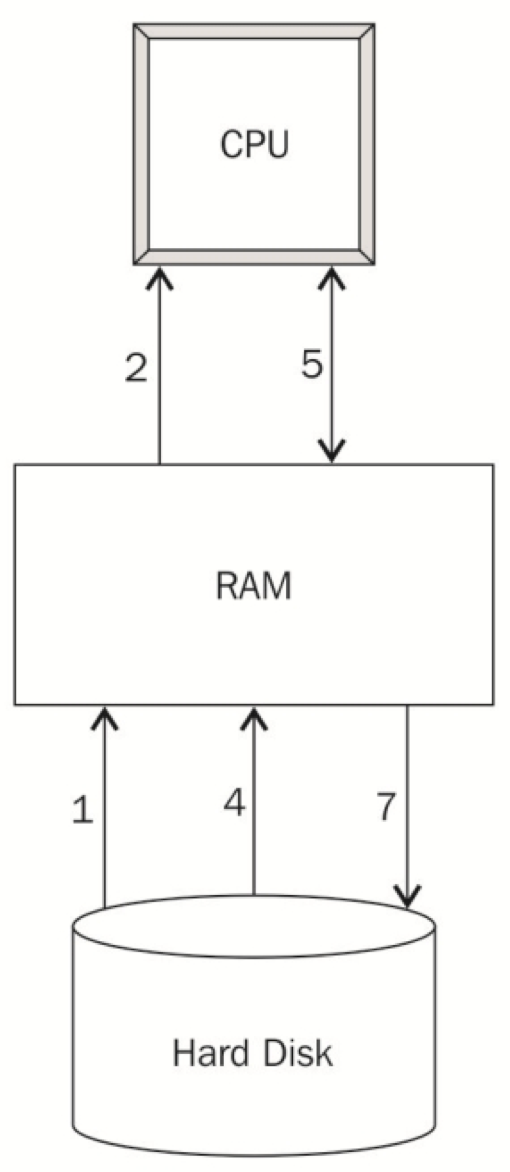
\includegraphics[width=7.08in]{images/ch1_bottlenecks} 

}

\caption{Steps to execute an R program, from @Lim2015, Chapter 1.}\label{fig:bottlenecks}
\end{figure}

\BeginKnitrBlock{exercise}
\protect\hypertarget{exr:unnamed-chunk-1}{}{\label{exr:unnamed-chunk-1} }Can
you identify points 1--7 in the following code snippet?
\EndKnitrBlock{exercise}

\begin{Shaded}
\begin{Highlighting}[]
\NormalTok{data <-}\StringTok{ }\KeywordTok{read.csv}\NormalTok{(}\StringTok{"mydata.csv"}\NormalTok{)}
\NormalTok{totals <-}\StringTok{ }\KeywordTok{colSums}\NormalTok{(data)}
\KeywordTok{write.csv}\NormalTok{(totals, }\StringTok{"totals.csv"}\NormalTok{)}
\end{Highlighting}
\end{Shaded}

\section{Syllabus}\label{syllabus}

Part I -- Good code still matters \emph{(even with lots of computing
resources)}

Week 1 - Basic tools

\begin{itemize}
\tightlist
\item
  Lecture 1. Unix scripting, make
\item
  Lecture 2. Version control: Git and GitHub (guest lecture: Ista Zhan)
\end{itemize}

Week 2 - Creating and maintaining R packages

\begin{itemize}
\tightlist
\item
  Lecture 3. Rationale, package structure, available tools
\item
  Lecture 4. Basics of software engineering: unit testing, code
  coverage, continuous integration
\end{itemize}

Week 3 - Software optimization

\begin{itemize}
\tightlist
\item
  Lecture 5. Measuring performance: profiling and benchmarking tools
\item
  Lecture 6. Improving performance: an introduction to C/C++, Rcpp
\end{itemize}

Part II -- Scaling up \emph{(don't use big data tools for small data)}

Week 4 -- Databases

\begin{itemize}
\tightlist
\item
  Lecture 7. Overview of SQL (SQLite, PostgreSQL) and noSQL databases
  (HBase, MongoDB, Cassandra, BigTable, \ldots{})
\item
  Lecture 8. R database interfaces (in particular through dplyr and
  mongolite)
\end{itemize}

Week 5 - Analyzing data that does not fit in memory

\begin{itemize}
\tightlist
\item
  Lecture 9. Pure R solutions (sampling, \texttt{ff} and
  \texttt{bigmemory}, other interpreters). JVM solutions (h20, Spark)
\item
  Lecture 10. An introduction to parallel computing; clusters and cloud
  computing. ``Divide and Conquer'' (MapReduce approaches)
\end{itemize}

Week 6 -- Visualization

\begin{itemize}
\tightlist
\item
  Lecture 11. Principles of visualization (guest lecture: James Honaker)
\item
  Lecture 12. Maps and GIS: principles of GIS, using R as a GIS, PostGIS
\end{itemize}

Weeks 7 \& 8 - Guest lectures (order and precise schedule TBD)

\begin{itemize}
\tightlist
\item
  Software project management (Danny Brooke)
\item
  R and Spark (Ellen Kraffmiller and Robert Treacy)
\item
  Advanced GIS and remote sensing (TBD)
\item
  Cluster architecture (William J. Horka)
\end{itemize}

\section{Evaluation}\label{evaluation}

Grades will be based on \textbf{two mandatory problem sets}. Each
problem set will correspond to 50\% (= 50 points) of the final grade.
The first problem set will be available by the end of week 3 and the
second problem set by the end of week 6.

You will be required to submit problem set solutions within two weeks.
Grades, and feedback when appropriate, will be returned two weeks after
submission.

You will submit a markdown document that combines commented code for
data analysis and detailed and structured explanations of the algorithms
and software tools that you used.

\section{Software tools and packages}\label{software-tools-and-packages}

We will mostly use \href{https://www.r-project.org/}{R} in this course.
Some examples will be run in \href{https://www.python.org/}{Python}.

In general, we will use free and open-source software programs such as
\href{https://www.postgresql.org/}{PostgreSQL} /
\href{http://postgis.net/}{PostGIS} or
\href{https://spark.apache.org/}{Spark}.

\section{Datasets}\label{datasets}

We have collected datasets to illustrate concepts. They are hosted on a
\href{https://www.dropbox.com/sh/mt4a7goxsl44swm/AADJK54wOXlDZjABMxN0DJIHa?dl=0}{Dropbox
folder}.

\subsection{MovieLens}\label{movielens}

MovieLens by
\citet[\url{https://grouplens.org/datasets/movielens/}]{Harper2015}
collects datasets from the website \url{https://movielens.org/}.

There are datasets of different sizes. We will use:

\begin{enumerate}
\def\labelenumi{\arabic{enumi}.}
\tightlist
\item
  Small (1MB): \url{https://grouplens.org/datasets/movielens/latest/}
\item
  Benchmark (\textasciitilde{}190MB zipped):
  \url{https://grouplens.org/datasets/movielens/20m/}
\end{enumerate}

\subsection{Airlines data}\label{airlines-data}

The airlines dataset comes from the U.S. Department of Transportation
and were used in the
\href{http://stat-computing.org/dataexpo/2009/}{2009 Data Expo} of the
American Statistical Association (ASA).

We will use a version curated by \href{https://www.h2o.ai/}{h2o}:
\url{https://github.com/h2oai/h2o-2/wiki/Hacking-Airline-DataSet-with-H2O}.

\subsection{Insurance claims}\label{insurance-claims}

Claims data contain Protected Health Information (PHI). There are strong
privacy restrictions to store, use and share this type of data.

We will use
\href{https://www.cms.gov/Research-Statistics-Data-and-Systems/Downloadable-Public-Use-Files/SynPUFs/DE_Syn_PUF.html}{synthetic
data}
(\href{https://www.cms.gov/Research-Statistics-Data-and-Systems/Downloadable-Public-Use-Files/SynPUFs/DESample01.html}{Sample
1}) from the Centers for Medicare and Medicaid Services (CMS).

\subsection{Census}\label{census}

Census data is commonly merged with administrative claims data such as
Medicare. We will use data from the
\href{https://www.census.gov/data.html}{Census Bureau}.

\subsection{\texorpdfstring{PM\textsubscript{2.5}
exposure}{PM2.5 exposure}}\label{pm2.5-exposure}

We will use PM\textsubscript{2.5} exposure data from the
\href{https://www.epa.gov/aqs}{EPA Air Quality System (AQS)} to
illustrate GIS linkage concepts.

\subsection{Methylation}\label{methylation}

If there is enough interest, we might present methylation examples.

\section{Contributing with GitHub}\label{contributing-with-github}

If you have suggestions, you can open a GitHub issue at
\url{https://github.com/cchoirat/bigdata17/issues}.

If you want to contribute, we welcome
\href{https://help.github.com/articles/about-pull-requests/}{pull
requests}.

\section{Before we start\ldots{}}\label{before-we-start}

How much R do you know?

Introduction to R:
\url{http://tutorials.iq.harvard.edu/R/Rintro/Rintro.html}

Regression models in R:
\url{http://tutorials.iq.harvard.edu/R/Rstatistics/Rstatistics.html}

R graphics:
\url{http://tutorials.iq.harvard.edu/R/Rgraphics/Rgraphics.html}

R programming:
\url{http://tutorials.iq.harvard.edu/R/RProgramming/Rprogramming.html}

\section{Style}\label{style}

Reading: \url{http://adv-r.had.co.nz/Style.html}

\chapter{Basic tools}\label{basics}

In this Chapter, we present basic tools that will be important when
interacting with big data systems: the command-line interface (CLI) in a
Unix shell and several utilities (\texttt{less}, \texttt{awk},
\texttt{vi} and \texttt{make}).

\section{Command line tools}\label{command-line-tools}

We assume some familiarity with the Unix shell, for example as in
\url{http://swcarpentry.github.io/shell-novice/}.

We also assume that you have access to a shell, either because you use
Linux or OS X or because you have the right tools on Windows (for
example \href{https://www.cygwin.com/}{Cygwin} or the Bash shell in
Windows 10).

\subsection{Why use the command line?}\label{why-use-the-command-line}

\begin{itemize}
\item
  Batch processing
\item
  Cluster and cloud computing
\end{itemize}

\subsection{Basic Unix tools}\label{basic-unix-tools}

\subsection{Useful tools}\label{useful-tools}

\subsubsection{\texorpdfstring{\texttt{less}}{less}}\label{less}

\texttt{less} is a pager that lets you view one page at a time files
that can be very large.

File \texttt{DE1\_0\_2008\_to\_2010\_Carrier\_Claims\_Sample\_1A.csv} in
\texttt{Data17/SyntheticMedicare} is 1.2GB. Even if we have enough RAM
to process the data, \texttt{less} helps get a very quick sense of the
data (variable names, separators, etc.)

\subsubsection{\texorpdfstring{\texttt{awk}}{awk}}\label{awk}

\texttt{awk} is a text-processing programming language available on most
Unix systems. It can be used for data extraction.

\subsubsection{\texorpdfstring{\texttt{vi}}{vi}}\label{vi}

\texttt{vi} is a screen-based text editor available on almost all Unix
systems. Most versions are actually
\href{http://www.vim.org/}{\texttt{Vim}} (that stands for ``Vi
IMproved'').

There are many cheat sheets and tutorials available on-line (for
example, the interactive \url{http://www.openvim.com/}). I invite you to
learn basics \texttt{vi} commands.

\subsection{Example}\label{example}

Let's apply some of the techniques described in \citet{Blackwell2012} on
Fisher's Iris data set saved in tab-delimited format. Of course, it is a
small dataset easily processed with R:

\begin{Shaded}
\begin{Highlighting}[]
\NormalTok{iris <-}\StringTok{ }\KeywordTok{read.table}\NormalTok{(}\StringTok{"~/Dropbox/Data17/iris/iris.tab"}\NormalTok{)}
\KeywordTok{head}\NormalTok{(iris, }\DataTypeTok{n =} \DecValTok{5}\NormalTok{)}
\end{Highlighting}
\end{Shaded}

\begin{verbatim}
##   Sepal.Length Sepal.Width Petal.Length Petal.Width Species
## 1          5.1         3.5          1.4         0.2  setosa
## 2          4.9         3.0          1.4         0.2  setosa
## 3          4.7         3.2          1.3         0.2  setosa
## 4          4.6         3.1          1.5         0.2  setosa
## 5          5.0         3.6          1.4         0.2  setosa
\end{verbatim}

In a shell, we can use:

\begin{Shaded}
\begin{Highlighting}[]
\FunctionTok{head}\NormalTok{ -n 6 ~/Dropbox/Data17/iris/iris.tab}
\end{Highlighting}
\end{Shaded}

\begin{verbatim}
## "Sepal.Length"   "Sepal.Width"   "Petal.Length"  "Petal.Width"   "Species"
## "1"  5.1 3.5 1.4 0.2 "setosa"
## "2"  4.9 3   1.4 0.2 "setosa"
## "3"  4.7 3.2 1.3 0.2 "setosa"
## "4"  4.6 3.1 1.5 0.2 "setosa"
## "5"  5   3.6 1.4 0.2 "setosa"
\end{verbatim}

Suppose we only need to select two variables in our model,
\texttt{Sepal.Length} and \texttt{Species}. In R, we can use:

\begin{Shaded}
\begin{Highlighting}[]
\NormalTok{iris_subset <-}\StringTok{ }\NormalTok{iris[, }\KeywordTok{c}\NormalTok{(}\StringTok{"Sepal.Length"}\NormalTok{, }\StringTok{"Species"}\NormalTok{)]}
\end{Highlighting}
\end{Shaded}

or

\begin{Shaded}
\begin{Highlighting}[]
\NormalTok{iris_subset <-}\StringTok{ }\NormalTok{iris[, }\KeywordTok{c}\NormalTok{(}\DecValTok{1}\NormalTok{, }\DecValTok{5}\NormalTok{)]}
\KeywordTok{head}\NormalTok{(iris_subset)}
\end{Highlighting}
\end{Shaded}

\begin{verbatim}
##   Sepal.Length Species
## 1          5.1  setosa
## 2          4.9  setosa
## 3          4.7  setosa
## 4          4.6  setosa
## 5          5.0  setosa
## 6          5.4  setosa
\end{verbatim}

With the tidyverse, we can use \emph{pipes}. The
\texttt{\%\textgreater{}\%} operator allows for performing chained
operations.

\begin{Shaded}
\begin{Highlighting}[]
\KeywordTok{suppressMessages}\NormalTok{(}\KeywordTok{library}\NormalTok{(dplyr))}

\NormalTok{iris }\OperatorTok
\StringTok{  }\KeywordTok{select}\NormalTok{(}\DecValTok{1}\NormalTok{, }\DecValTok{5}\NormalTok{) }\OperatorTok\StringTok{ }
\StringTok{  }\KeywordTok{head}\NormalTok{()}
\end{Highlighting}
\end{Shaded}

\begin{verbatim}
##   Sepal.Length Species
## 1          5.1  setosa
## 2          4.9  setosa
## 3          4.7  setosa
## 4          4.6  setosa
## 5          5.0  setosa
## 6          5.4  setosa
\end{verbatim}

In a shell, the pipe operator to combine shell commands is
\texttt{\textbar{}} and we can use:

\begin{Shaded}
\begin{Highlighting}[]
\FunctionTok{cut}\NormalTok{ -f 1,5 ~/Dropbox/Data17/iris/iris.tab }\KeywordTok{|} \FunctionTok{head}\NormalTok{ -n 7}
\end{Highlighting}
\end{Shaded}

\begin{verbatim}
## "Sepal.Length"   "Species"
## "1"  0.2
## "2"  0.2
## "3"  0.2
## "4"  0.2
## "5"  0.2
## "6"  0.4
\end{verbatim}

To keep observations with ``Sepal.Length'' greater than 5:

\begin{Shaded}
\begin{Highlighting}[]
\NormalTok{iris }\OperatorTok
\StringTok{  }\KeywordTok{filter}\NormalTok{(Sepal.Length }\OperatorTok{>}\StringTok{ }\DecValTok{5}\NormalTok{) }\OperatorTok\StringTok{ }
\StringTok{  }\KeywordTok{head}\NormalTok{()}
\end{Highlighting}
\end{Shaded}

\begin{verbatim}
##   Sepal.Length Sepal.Width Petal.Length Petal.Width Species
## 1          5.1         3.5          1.4         0.2  setosa
## 2          5.4         3.9          1.7         0.4  setosa
## 3          5.4         3.7          1.5         0.2  setosa
## 4          5.8         4.0          1.2         0.2  setosa
## 5          5.7         4.4          1.5         0.4  setosa
## 6          5.4         3.9          1.3         0.4  setosa
\end{verbatim}

In the shell, we can use the \texttt{AWK} programming language. We start
from row \texttt{NR} 2 (we could start from row 1, it contains variable
names) and select rows such that the second variable
(\texttt{Sepal.Length}) is greater than 5.

\begin{Shaded}
\begin{Highlighting}[]
\FunctionTok{awk} \StringTok{'NR == 2 || $2 > 5'}\NormalTok{ ~/Dropbox/Data17/iris/iris.tab }\KeywordTok{|} \FunctionTok{head}
\end{Highlighting}
\end{Shaded}

\begin{verbatim}
## "1"  5.1 3.5 1.4 0.2 "setosa"
## "6"  5.4 3.9 1.7 0.4 "setosa"
## "11" 5.4 3.7 1.5 0.2 "setosa"
## "15" 5.8 4   1.2 0.2 "setosa"
## "16" 5.7 4.4 1.5 0.4 "setosa"
## "17" 5.4 3.9 1.3 0.4 "setosa"
## "18" 5.1 3.5 1.4 0.3 "setosa"
## "19" 5.7 3.8 1.7 0.3 "setosa"
## "20" 5.1 3.8 1.5 0.3 "setosa"
## "21" 5.4 3.4 1.7 0.2 "setosa"
\end{verbatim}

\BeginKnitrBlock{exercise}
\protect\hypertarget{exr:unnamed-chunk-11}{}{\label{exr:unnamed-chunk-11}
}The iris dataset is also saved in .csv format at
\texttt{\textasciitilde{}/Dropbox/Data17/iris/iris.csv}. Use
\texttt{AWK} and \texttt{tail} to select the last 5 observations where
\texttt{Sepal.Width} is larger than 3.5 and \texttt{Petal.Length} is
smaller than 1.5.
\EndKnitrBlock{exercise}

\section{Makefiles}\label{makefiles}

\texttt{make} is a tool that helps put all the (interdependent) pieces
of an analytic workflow together:

\begin{itemize}
\tightlist
\item
  data retrieving
\item
  data cleaning
\item
  analysis
\item
  graphs
\item
  reports
\item
  \ldots{}
\end{itemize}

\subsection{Simulate data in R}\label{simulate-data-in-r}

\begin{Shaded}
\begin{Highlighting}[]
\KeywordTok{set.seed}\NormalTok{(}\DecValTok{123}\NormalTok{)}
\end{Highlighting}
\end{Shaded}

File \texttt{simulate\_data.R}

\begin{Shaded}
\begin{Highlighting}[]
\CommentTok{# set.seed(123)}
\NormalTok{N <-}\StringTok{ }\DecValTok{1000} \CommentTok{# sample size}

\NormalTok{X1 <-}\StringTok{ }\KeywordTok{rpois}\NormalTok{(}\DataTypeTok{n =}\NormalTok{ N, }\DataTypeTok{lambda =} \DecValTok{50}\NormalTok{)}
\NormalTok{X2 <-}\StringTok{ }\DecValTok{10} \OperatorTok{+}\StringTok{ }\KeywordTok{rbinom}\NormalTok{(}\DataTypeTok{n =}\NormalTok{ N, }\DataTypeTok{prob =} \FloatTok{0.8}\NormalTok{, }\DataTypeTok{size =} \DecValTok{1}\NormalTok{)}
\NormalTok{Y <-}\StringTok{ }\DecValTok{10} \OperatorTok{+}\StringTok{ }\DecValTok{3} \OperatorTok{*}\StringTok{ }\NormalTok{X1 }\OperatorTok{+}\StringTok{ }\OperatorTok{-}\DecValTok{5} \OperatorTok{*}\StringTok{ }\NormalTok{X2 }\OperatorTok{+}\StringTok{ }\DecValTok{3} \OperatorTok{*}\StringTok{ }\KeywordTok{rnorm}\NormalTok{(}\DataTypeTok{n =}\NormalTok{ N)}

\KeywordTok{write.csv}\NormalTok{(}\KeywordTok{data.frame}\NormalTok{(}\DataTypeTok{Y =}\NormalTok{ Y, }\DataTypeTok{X1 =}\NormalTok{ X1, }\DataTypeTok{X2 =}\NormalTok{ X2),}
          \StringTok{"sample_data.csv"}\NormalTok{, }\DataTypeTok{row.names =} \OtherTok{FALSE}\NormalTok{)}
\end{Highlighting}
\end{Shaded}

\begin{Shaded}
\begin{Highlighting}[]
\KeywordTok{head}\NormalTok{(}\KeywordTok{data.frame}\NormalTok{(}\DataTypeTok{Y =}\NormalTok{ Y, }\DataTypeTok{X1 =}\NormalTok{ X1, }\DataTypeTok{X2 =}\NormalTok{ X2))}
\end{Highlighting}
\end{Shaded}

\begin{verbatim}
##           Y X1 X2
## 1  88.74430 46 11
## 2 125.77081 58 11
## 3  70.76396 38 10
## 4 110.32157 50 10
## 5 145.79546 62 11
## 6 109.45403 53 11
\end{verbatim}

\subsection{Create a plot in Python}\label{create-a-plot-in-python}

File \texttt{create\_graph.py}

\begin{Shaded}
\begin{Highlighting}[]
\ImportTok{import}\NormalTok{ pandas }\ImportTok{as}\NormalTok{ pd}
\ImportTok{import}\NormalTok{ matplotlib.pyplot }\ImportTok{as}\NormalTok{ plt}

\NormalTok{sim_data }\OperatorTok{=}\NormalTok{ pd.read_csv(}\StringTok{"sample_data.csv"}\NormalTok{)}

\NormalTok{plt.figure()}
\NormalTok{sim_data.plot()}
\NormalTok{plt.savefig(}\StringTok{"plot.pdf"}\NormalTok{, }\BuiltInTok{format} \OperatorTok{=} \StringTok{"pdf"}\NormalTok{)}
\end{Highlighting}
\end{Shaded}

\includegraphics[width=53.33in]{images/ch1_plot}

\subsection{Run statistical model in
R}\label{run-statistical-model-in-r}

We can estimate the model with R:

\begin{Shaded}
\begin{Highlighting}[]
\NormalTok{sim_data <-}\StringTok{ }\KeywordTok{read.csv}\NormalTok{(}\StringTok{"sample_data.csv"}\NormalTok{)}
\KeywordTok{summary}\NormalTok{(}\KeywordTok{lm}\NormalTok{(Y }\OperatorTok{~}\StringTok{ }\NormalTok{X1 }\OperatorTok{+}\StringTok{ }\NormalTok{X2, }\DataTypeTok{data =}\NormalTok{ sim_data))}
\end{Highlighting}
\end{Shaded}

\begin{verbatim}
## 
## Call:
## lm(formula = Y ~ X1 + X2, data = sim_data)
## 
## Residuals:
##     Min      1Q  Median      3Q     Max 
## -8.3988 -1.9452 -0.0261  2.0216  9.1066 
## 
## Coefficients:
##             Estimate Std. Error t value Pr(>|t|)    
## (Intercept)  9.09087    2.54667    3.57 0.000374 ***
## X1           3.00531    0.01326  226.68  < 2e-16 ***
## X2          -4.94658    0.22876  -21.62  < 2e-16 ***
## ---
## Signif. codes:  0 '***' 0.001 '**' 0.01 '*' 0.05 '.' 0.1 ' ' 1
## 
## Residual standard error: 2.936 on 997 degrees of freedom
## Multiple R-squared:  0.9811, Adjusted R-squared:  0.981 
## F-statistic: 2.585e+04 on 2 and 997 DF,  p-value: < 2.2e-16
\end{verbatim}

\subsection{Run statistical model in
R}\label{run-statistical-model-in-r-1}

To save the output, we use the \texttt{sink} function.

File \texttt{estimate\_model.R}

\begin{Shaded}
\begin{Highlighting}[]
\KeywordTok{sink}\NormalTok{(}\StringTok{"estimation_summary.txt"}\NormalTok{)}
\KeywordTok{summary}\NormalTok{(}\KeywordTok{lm}\NormalTok{(Y }\OperatorTok{~}\StringTok{ }\NormalTok{X1 }\OperatorTok{+}\StringTok{ }\NormalTok{X2, }\DataTypeTok{data =}\NormalTok{ sim_data))}
\KeywordTok{sink}\NormalTok{()}
\end{Highlighting}
\end{Shaded}

\subsection{Makefile syntax}\label{makefile-syntax}

\begin{itemize}
\item
  \texttt{make} is a \emph{command} that runs on a text file often named
  \texttt{Makefile}.
\item
  A \texttt{Makefile} contains one or several blocks with the following
  structure:
\end{itemize}

\begin{verbatim}
targetfile: sourcefile(s)
[tab] command
\end{verbatim}

\subsection{Naive version}\label{naive-version}

File: \texttt{Makefile}

\begin{verbatim}
sample_data.csv: simulate_data.R
    R CMD BATCH simulate_data.R

plot.pdf: create_graph.py
    python create_graph.py

estimation_summary.txt: estimate_model.R
    R CMD BATCH estimate_model.R
\end{verbatim}

A simple call to \texttt{make} only builds the first target
(\texttt{sample\_data.csv}). To build the other targets, we have to use:
\texttt{make\ plot.pdf} and \texttt{make\ estimation\_summary.txt}.

\subsection{Making all targets}\label{making-all-targets}

File: \texttt{Makefile}

\begin{verbatim}
all: analysis

analysis: sample_data.csv plot.pdf estimation_summary.txt

sample_data.csv: simulate_data.R
    R CMD BATCH simulate_data.R

plot.pdf: create_graph.py
    python create_graph.py

estimation_summary.txt: estimate_model.R
    R CMD BATCH estimate_model.R
\end{verbatim}

New data is simulated and saved in \texttt{sample\_data.csv}. But
\texttt{plot.pdf} and \texttt{estimation\_summary.txt} are not updated.

\subsection{Dealing with dependencies}\label{dealing-with-dependencies}

\begin{itemize}
\tightlist
\item
  Problem \texttt{plot.pdf} and \texttt{estimation\_summary.txt} depend
  on \texttt{sample\_data.csv}.
\item
  Solution: explicit dependencies.
\end{itemize}

File: \texttt{Makefile}

\begin{verbatim}
all: analysis

analysis: sample_data.csv plot.pdf estimation_summary.txt

sample_data.csv: simulate_data.R
    R CMD BATCH simulate_data.R

plot.pdf: sample_data.csv create_graph.py
    python create_graph.py

estimation_summary.txt: sample_data.csv estimate_model.R
    R CMD BATCH estimate_model.R
\end{verbatim}

\section{Git and GitHub}\label{git-and-github}

Guest lecture by \href{https://www.iq.harvard.edu/people/ista-zahn}{Ista
Zahn}.

\chapter{Packages}\label{packages}

We strongly recommand \citet{Wickham2015}.

We assume the following packages are installed:

\begin{Shaded}
\begin{Highlighting}[]
\KeywordTok{install.packages}\NormalTok{(}\KeywordTok{c}\NormalTok{(}\StringTok{"devtools"}\NormalTok{, }\StringTok{"roxygen2"}\NormalTok{, }\StringTok{"testthat"}\NormalTok{, }\StringTok{"knitr"}\NormalTok{))}
\end{Highlighting}
\end{Shaded}

\section{Why?}\label{why}

\begin{itemize}
\item
  Organize your code
\item
  Distribute your code
\item
  Keep versions of your code
\end{itemize}

\section{Package structure}\label{package-structure}

\begin{itemize}
\tightlist
\item
  Folder hierarchy

  \begin{itemize}
  \tightlist
  \item
    \texttt{NAMESPACE}: package import / export
  \item
    \texttt{DESCRIPTION}: metadata
  \item
    \texttt{R/}: R code
  \item
    \texttt{man/}: object documentation (with short examples)
  \item
    \texttt{tests/}
  \item
    \texttt{data/}
  \item
    \texttt{src/}: compiled code
  \item
    \texttt{vignettes/}: manual-like documentation
  \item
    \texttt{inst/}: installed files
  \item
    \texttt{demo/}: longer examples
  \item
    \texttt{exec}, \texttt{po}, \texttt{tools}
  \end{itemize}
\end{itemize}

\section{Building steps}\label{building-steps}

\begin{itemize}
\item
  \texttt{R\ CMD\ build}
\item
  \texttt{R\ CMD\ INSTALL}
\item
  \texttt{R\ CMD\ check}
\end{itemize}

\subsection{\texorpdfstring{\texttt{R\ CMD\ build}}{R CMD build}}\label{r-cmd-build}

\begin{Shaded}
\begin{Highlighting}[]
\NormalTok{R CMD build }\OperatorTok{--}\NormalTok{help}
\end{Highlighting}
\end{Shaded}

\emph{Build R packages from package sources in the directories specified
by `pkgdirs'}

\subsection{\texorpdfstring{\texttt{R\ CMD\ INSTALL}}{R CMD INSTALL}}\label{r-cmd-install}

\begin{Shaded}
\begin{Highlighting}[]
\NormalTok{R CMD INSTALL }\OperatorTok{--}\NormalTok{help}
\end{Highlighting}
\end{Shaded}

\emph{Install the add-on packages specified by pkgs. The elements of
pkgs can be relative or absolute paths to directories with the package
sources, or to gzipped package `tar' archives. The library tree to
install to can be specified via `--library'. By default, packages are
installed in the library tree rooted at the first directory in
.libPaths() for an R session run in the current environment.}

\subsection{\texorpdfstring{\texttt{R\ CMD\ check}}{R CMD check}}\label{r-cmd-check}

\begin{Shaded}
\begin{Highlighting}[]
\NormalTok{R CMD check }\OperatorTok{--}\NormalTok{help}
\end{Highlighting}
\end{Shaded}

\url{http://r-pkgs.had.co.nz/check.html}

\emph{Check R packages from package sources, which can be directories or
package `tar' archives with extension `.tar.gz', `.tar.bz2', `.tar.xz'
or `.tgz'.}

\emph{A variety of diagnostic checks on directory structure, index and
control files are performed. The package is installed into the log
directory and production of the package PDF manual is tested. All
examples and tests provided by the package are tested to see if they run
successfully. By default code in the vignettes is tested, as is
re-building the vignette PDFs.}

\subsection{\texorpdfstring{Building steps with
\texttt{devtools}}{Building steps with devtools}}\label{building-steps-with-devtools}

\begin{itemize}
\item
  \texttt{devtools::build}
\item
  \texttt{devtools::install}
\item
  \texttt{devtools::check}
\item
  and many others: \texttt{load\_all}, \texttt{document}, \texttt{test},
  \texttt{run\_examples}, \ldots{}
\end{itemize}

\section{Create an R package}\label{create-an-r-package}

\subsection{\texorpdfstring{\texttt{utils::package.skeleton}}{utils::package.skeleton}}\label{utilspackage.skeleton}

\begin{Shaded}
\begin{Highlighting}[]
\KeywordTok{package.skeleton}\NormalTok{() }\CommentTok{# "in "clean" session ("anRpackage")}
\KeywordTok{package.skeleton}\NormalTok{(}\StringTok{"pkgname"}\NormalTok{) }\CommentTok{# in "clean" session}

\KeywordTok{set.seed}\NormalTok{(}\DecValTok{02138}\NormalTok{)}
\NormalTok{f <-}\StringTok{ }\ControlFlowTok{function}\NormalTok{(x, y) x}\OperatorTok{+}\NormalTok{y}
\NormalTok{g <-}\StringTok{ }\ControlFlowTok{function}\NormalTok{(x, y) x}\OperatorTok{-}\NormalTok{y}
\NormalTok{d <-}\StringTok{ }\KeywordTok{data.frame}\NormalTok{(}\DataTypeTok{a =} \DecValTok{1}\NormalTok{, }\DataTypeTok{b =} \DecValTok{2}\NormalTok{)}
\NormalTok{e <-}\StringTok{ }\KeywordTok{rnorm}\NormalTok{(}\DecValTok{1000}\NormalTok{)}
\KeywordTok{package.skeleton}\NormalTok{(}\DataTypeTok{list =} \KeywordTok{c}\NormalTok{(}\StringTok{"f"}\NormalTok{,}\StringTok{"g"}\NormalTok{,}\StringTok{"d"}\NormalTok{,}\StringTok{"e"}\NormalTok{), }\DataTypeTok{name =} \StringTok{"pkgname"}\NormalTok{)}
\end{Highlighting}
\end{Shaded}

\subsection{\texorpdfstring{\texttt{devtools::create}}{devtools::create}}\label{devtoolscreate}

\begin{Shaded}
\begin{Highlighting}[]
\NormalTok{devtools}\OperatorTok{::}\KeywordTok{create}\NormalTok{(}\StringTok{"path/to/package/pkgname"}\NormalTok{)}
\end{Highlighting}
\end{Shaded}

Also from RStudio (`File -\textgreater{} New Project').

\subsection{Submit to CRAN}\label{submit-to-cran}

\begin{figure}

{\centering 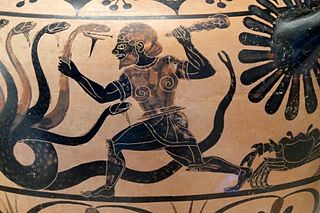
\includegraphics[width=4.44in]{images/ch3_hydra} 

}

\caption{Submitting to CRAN.  It's not that bad...}\label{fig:hydra}
\end{figure}

Reading: \url{http://r-pkgs.had.co.nz/release.html}

\section{R packages on GitHub}\label{r-packages-on-github}

Reading: \url{http://r-pkgs.had.co.nz/git.html}

\begin{itemize}
\item
  Version control
\item
  Website, wiki, project management
\item
  Easy install: \texttt{install\_github} from \texttt{devtools}
\item
  Collaboration
\item
  Issue tracking
\end{itemize}

\subsubsection{RStudio and GitHub
integration}\label{rstudio-and-github-integration}

\begin{figure}

{\centering 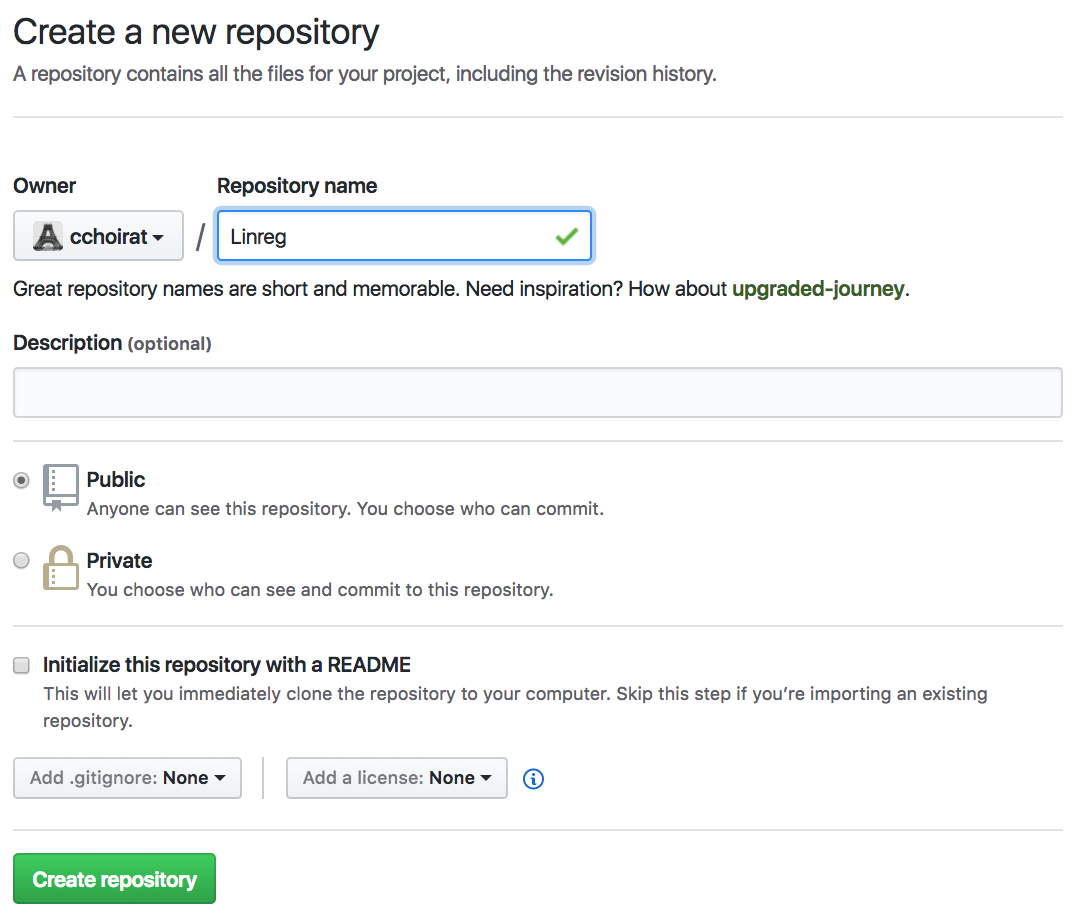
\includegraphics[width=15in]{images/ch3_pkg_1_github} 

}

\caption{Create a new Linreg repository on GitHub}\label{fig:pkg1}
\end{figure}

\begin{figure}

{\centering 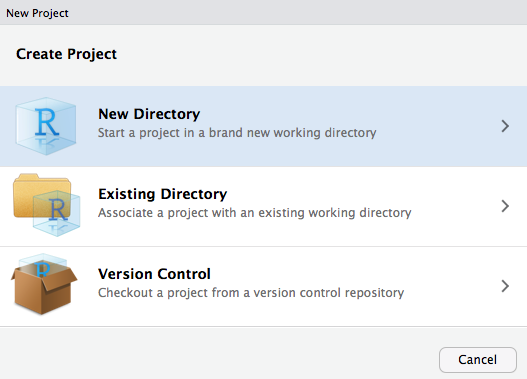
\includegraphics[width=7.32in]{images/ch3_pkg_2_project} 

}

\caption{Create a new project in RStudio}\label{fig:pkg2}
\end{figure}

\begin{figure}

{\centering 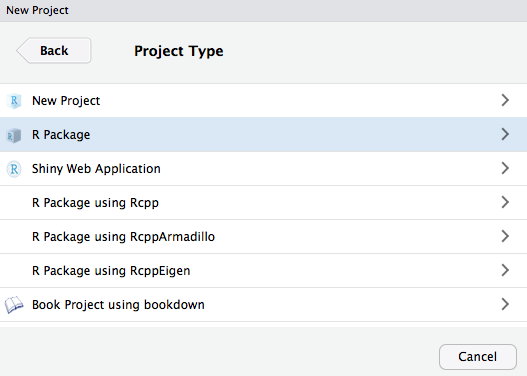
\includegraphics[width=7.32in]{images/ch3_pkg_3_package} 

}

\caption{Select R package}\label{fig:pkg3}
\end{figure}

\begin{figure}

{\centering 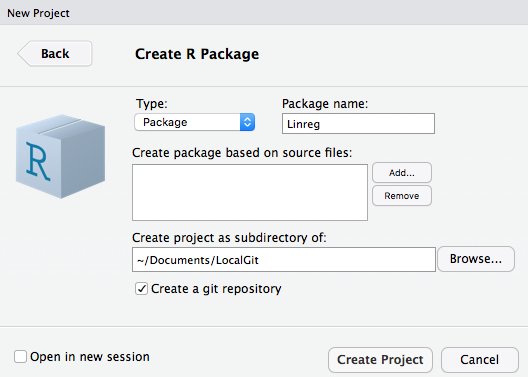
\includegraphics[width=7.33in]{images/ch3_pkg_4_create} 

}

\caption{Create the Linreg R package as a Git repository}\label{fig:pkg4}
\end{figure}

\begin{figure}

{\centering 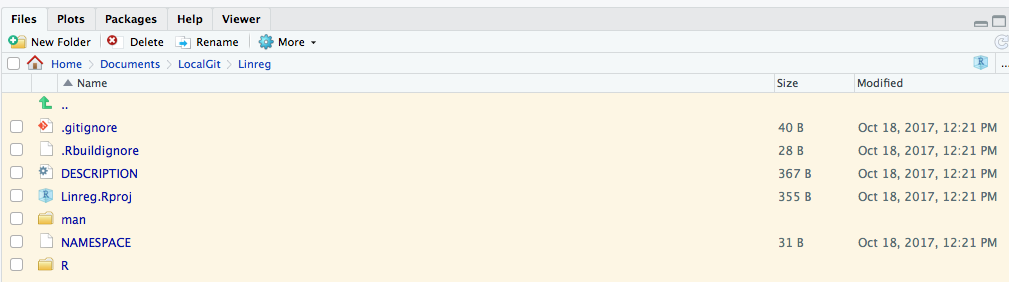
\includegraphics[width=14.01in]{images/ch3_pkg_5_filelist} 

}

\caption{Automatically created files}\label{fig:pkg5}
\end{figure}

\begin{figure}

{\centering 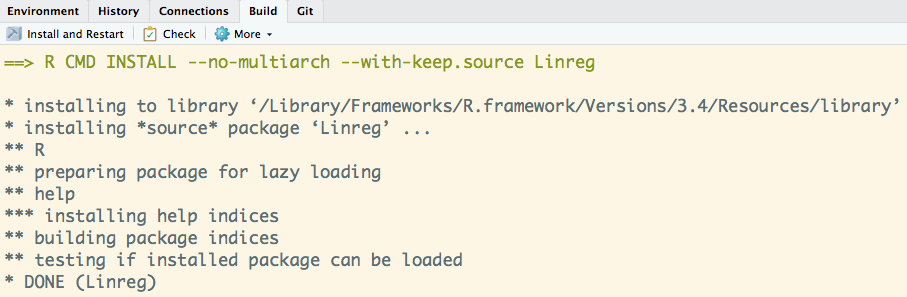
\includegraphics[width=12.6in]{images/ch3_pkg_6_install} 

}

\caption{Build tab in RStudio}\label{fig:pkg6}
\end{figure}

\begin{figure}

{\centering 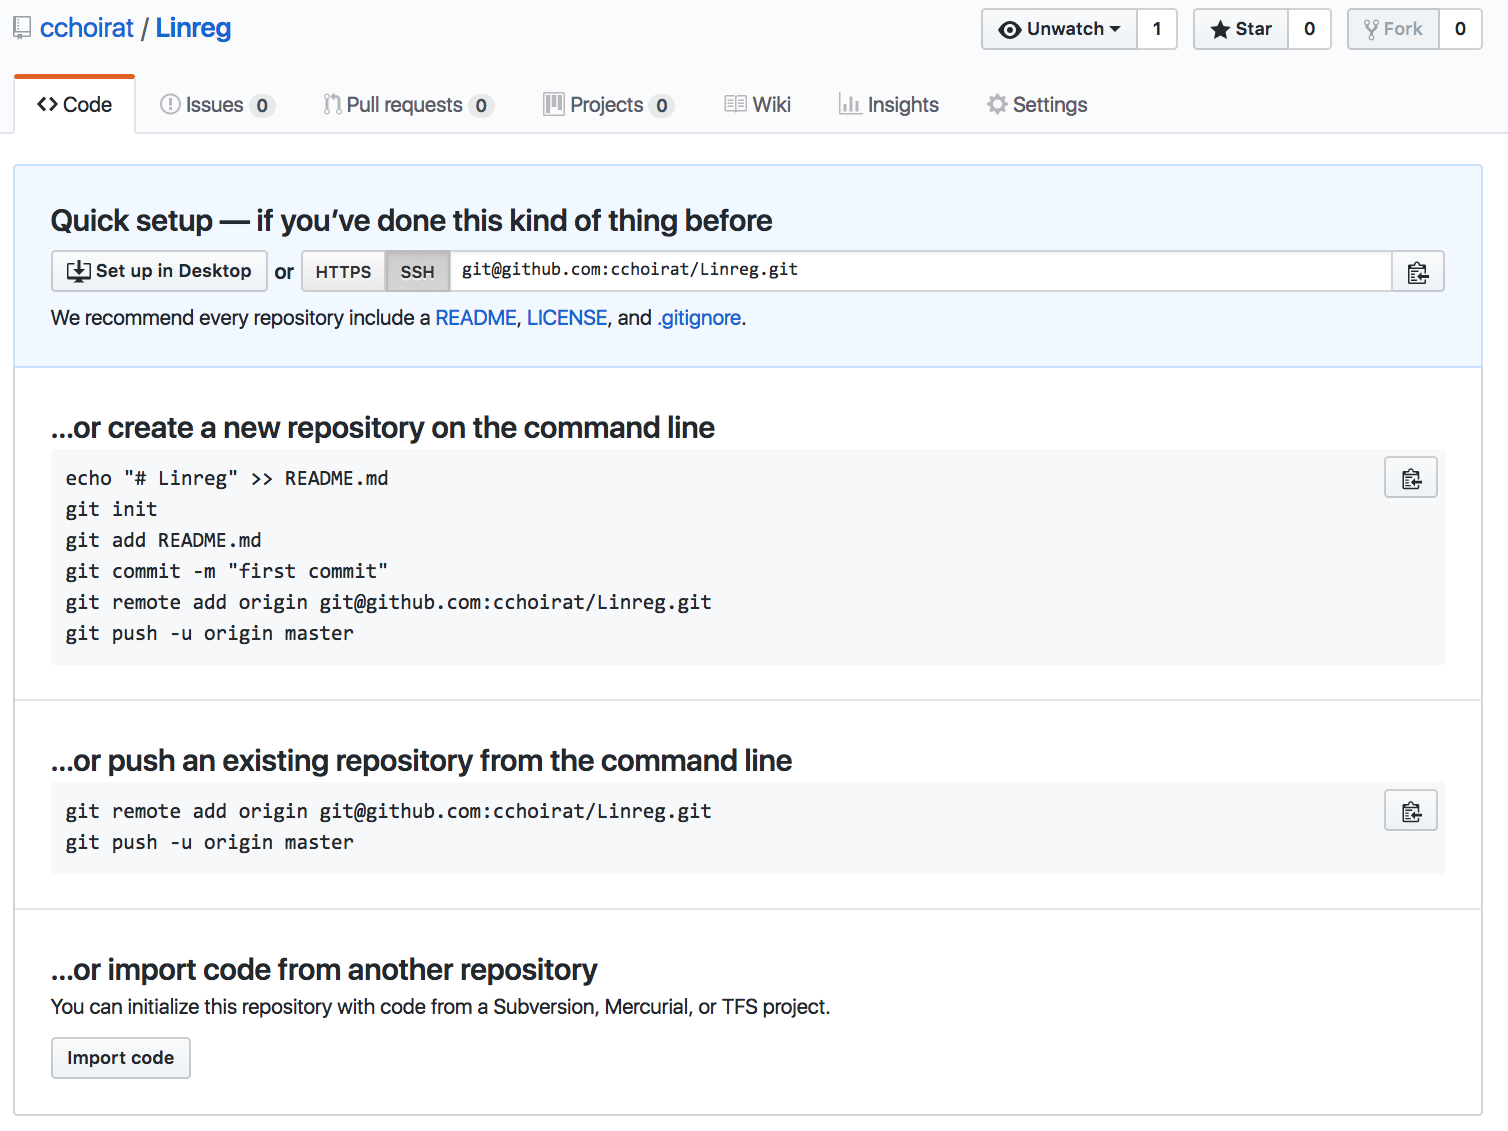
\includegraphics[width=20.94in]{images/ch3_pkg_7_github} 

}

\caption{Github webpage}\label{fig:pkg7}
\end{figure}

\begin{figure}

{\centering 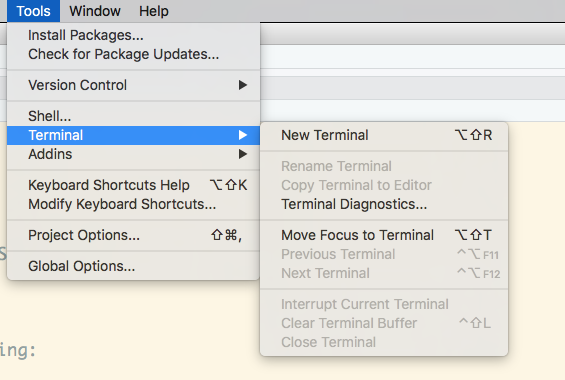
\includegraphics[width=7.85in]{images/ch3_pkg_8_terminal} 

}

\caption{Open a terminal}\label{fig:term}
\end{figure}

\textbf{Command line}

\begin{Shaded}
\begin{Highlighting}[]
\CommentTok{# git init # already run when creating package with RStudio}
\NormalTok{git add }\OperatorTok{*}
\NormalTok{git commit }\OperatorTok{-}\NormalTok{m }\StringTok{"First commit"}
\NormalTok{git remote add origin https}\OperatorTok{:}\ErrorTok{//}\NormalTok{github.com}\OperatorTok{/}\NormalTok{cchoirat}\OperatorTok{/}\NormalTok{Linreg}
\NormalTok{git push }\OperatorTok{-}\NormalTok{u origin master}
\end{Highlighting}
\end{Shaded}

\begin{figure}

{\centering 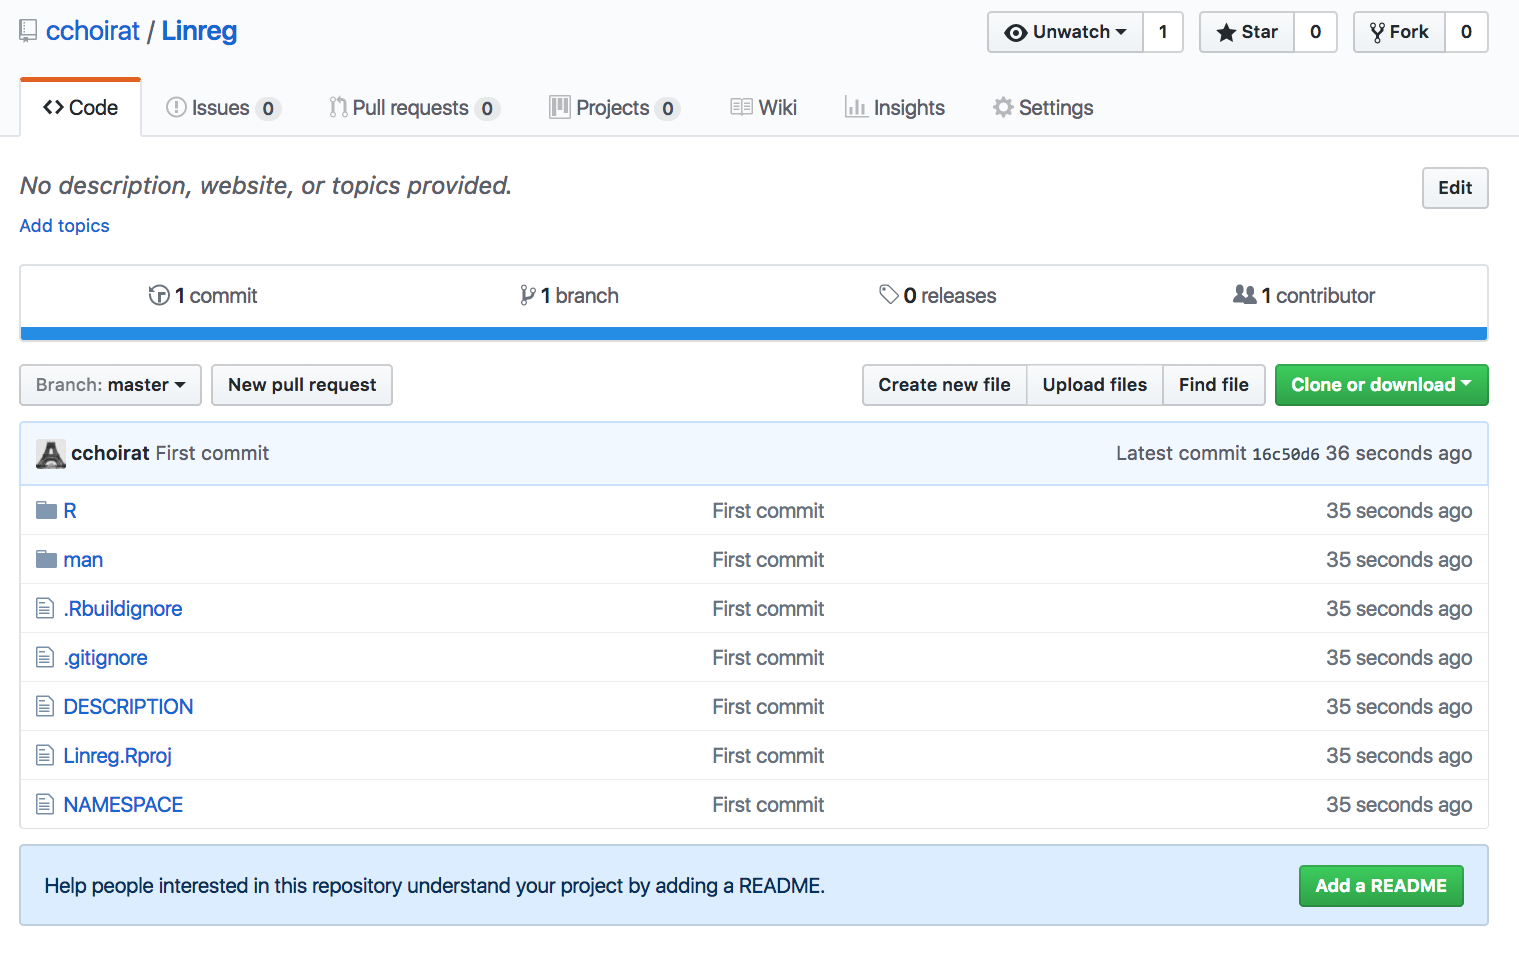
\includegraphics[width=21.1in]{images/ch3_pkg_9_github} 

}

\caption{Github webpage is updated}\label{fig:pkg9}
\end{figure}

\subsection{\texorpdfstring{\texttt{.gitignore}}{.gitignore}}\label{gitignore}

RStudio default

\begin{Shaded}
\begin{Highlighting}[]
\NormalTok{.Rproj.user}
\NormalTok{.Rhistory}
\NormalTok{.RData}
\end{Highlighting}
\end{Shaded}

GitHub default

\begin{Shaded}
\begin{Highlighting}[]
\CommentTok{# History files}
\NormalTok{.Rhistory}
\NormalTok{.Rapp.history}

\CommentTok{# Example code in package build process}
\OperatorTok{*-}\NormalTok{Ex.R}

\CommentTok{# RStudio files}
\NormalTok{.Rproj.user}\OperatorTok{/}

\CommentTok{# produced vignettes}
\NormalTok{vignettes}\OperatorTok{/}\ErrorTok{*}\NormalTok{.html}
\NormalTok{vignettes}\OperatorTok{/}\ErrorTok{*}\NormalTok{.pdf}
\end{Highlighting}
\end{Shaded}

\section{RStudio projects}\label{rstudio-projects}

\begin{itemize}
\item
  \texttt{.Rproj} file extension, in our example \texttt{Linreg.Rproj}
\item
  A project has its own:

  \begin{itemize}
  \tightlist
  \item
    R session
  \item
    .Rprofile (\emph{e.g.}, to customize startup environment)
  \item
    .Rhistory
  \end{itemize}
\item
  Default working directory is project directory
\item
  Keeps track of project-specific recent files
\end{itemize}

\subsection{Project options}\label{project-options}

\begin{Shaded}
\begin{Highlighting}[]
\NormalTok{Version}\OperatorTok{:}\StringTok{ }\FloatTok{1.0}

\NormalTok{RestoreWorkspace}\OperatorTok{:}\StringTok{ }\NormalTok{Default}
\NormalTok{SaveWorkspace}\OperatorTok{:}\StringTok{ }\NormalTok{Default}
\NormalTok{AlwaysSaveHistory}\OperatorTok{:}\StringTok{ }\NormalTok{Default}

\NormalTok{EnableCodeIndexing}\OperatorTok{:}\StringTok{ }\NormalTok{Yes}
\NormalTok{UseSpacesForTab}\OperatorTok{:}\StringTok{ }\NormalTok{Yes}
\NormalTok{NumSpacesForTab}\OperatorTok{:}\StringTok{ }\DecValTok{2}
\NormalTok{Encoding}\OperatorTok{:}\StringTok{ }\NormalTok{UTF}\OperatorTok{-}\DecValTok{8}

\NormalTok{RnwWeave}\OperatorTok{:}\StringTok{ }\NormalTok{knitr}
\NormalTok{LaTeX}\OperatorTok{:}\StringTok{ }\NormalTok{pdfLaTeX}

\NormalTok{AutoAppendNewline}\OperatorTok{:}\StringTok{ }\NormalTok{Yes}
\NormalTok{StripTrailingWhitespace}\OperatorTok{:}\StringTok{ }\NormalTok{Yes}

\NormalTok{BuildType}\OperatorTok{:}\StringTok{ }\NormalTok{Package}
\NormalTok{PackageUseDevtools}\OperatorTok{:}\StringTok{ }\NormalTok{Yes}
\NormalTok{PackageInstallArgs}\OperatorTok{:}\StringTok{ }\OperatorTok{--}\NormalTok{no}\OperatorTok{-}\NormalTok{multiarch }\OperatorTok{--}\NormalTok{with}\OperatorTok{-}\NormalTok{keep.source}
\end{Highlighting}
\end{Shaded}

\subsection{Package documentation}\label{package-documentation}

\begin{itemize}
\item
  Functions and methods
\item
  Vignettes

  \begin{itemize}
  \tightlist
  \item
    PDF
  \item
    \texttt{knitr}
  \end{itemize}
\end{itemize}

\section{Package workflow example}\label{package-workflow-example}

Creating R Packages: A Tutorial (Friedrich Leisch, 2009)

Our example is adapted from
\url{https://cran.r-project.org/doc/contrib/Leisch-CreatingPackages.pdf}.

\subsection{\texorpdfstring{Add \texttt{linreg.R} to \texttt{R/}
directory}{Add linreg.R to R/ directory}}\label{add-linreg.r-to-r-directory}

\begin{Shaded}
\begin{Highlighting}[]
\NormalTok{linmodEst <-}\StringTok{ }\ControlFlowTok{function}\NormalTok{(x, y) \{}
\NormalTok{  ## CC: crossprod or a QR decomposition (as in the original version) are more efficient}
\NormalTok{  coef <-}\StringTok{ }\KeywordTok{solve}\NormalTok{(}\KeywordTok{t}\NormalTok{(x) }\OperatorTok\StringTok{ }\NormalTok{x) }\OperatorTok\StringTok{ }\KeywordTok{t}\NormalTok{(x) }\OperatorTok\StringTok{ }\NormalTok{y}
  \KeywordTok{print}\NormalTok{(coef)}
\NormalTok{  ## degrees of freedom and standard deviation of residuals}
\NormalTok{  df <-}\StringTok{ }\KeywordTok{nrow}\NormalTok{(x) }\OperatorTok{-}\StringTok{ }\KeywordTok{ncol}\NormalTok{(x)}
\NormalTok{  sigma2 <-}\StringTok{ }\KeywordTok{sum}\NormalTok{((y }\OperatorTok{-}\StringTok{ }\NormalTok{x }\OperatorTok\StringTok{ }\NormalTok{coef) }\OperatorTok{^}\StringTok{ }\DecValTok{2}\NormalTok{) }\OperatorTok{/}\StringTok{ }\NormalTok{df}
\NormalTok{  ## compute sigma^2 * (x’x)^-1}
\NormalTok{  vcov <-}\StringTok{ }\NormalTok{sigma2 }\OperatorTok{*}\StringTok{ }\KeywordTok{solve}\NormalTok{(}\KeywordTok{t}\NormalTok{(x) }\OperatorTok\StringTok{ }\NormalTok{x)}
  \KeywordTok{colnames}\NormalTok{(vcov) <-}\StringTok{ }\KeywordTok{rownames}\NormalTok{(vcov) <-}\StringTok{ }\KeywordTok{colnames}\NormalTok{(x)}
  \KeywordTok{list}\NormalTok{(}
    \DataTypeTok{coefficients =}\NormalTok{ coef,}
    \DataTypeTok{vcov =}\NormalTok{ vcov,}
    \DataTypeTok{sigma =} \KeywordTok{sqrt}\NormalTok{(sigma2),}
    \DataTypeTok{df =}\NormalTok{ df}
\NormalTok{  )}
\NormalTok{\}}
\end{Highlighting}
\end{Shaded}

\subsection{Run our function}\label{run-our-function}

\begin{Shaded}
\begin{Highlighting}[]
\KeywordTok{data}\NormalTok{(cats, }\DataTypeTok{package =} \StringTok{"MASS"}\NormalTok{)}
\KeywordTok{linmodEst}\NormalTok{(}\KeywordTok{cbind}\NormalTok{(}\DecValTok{1}\NormalTok{, cats}\OperatorTok{$}\NormalTok{Bwt), cats}\OperatorTok{$}\NormalTok{Hwt)}
\end{Highlighting}
\end{Shaded}

\begin{verbatim}
##            [,1]
## [1,] -0.3566624
## [2,]  4.0340627
\end{verbatim}

\begin{verbatim}
## $coefficients
##            [,1]
## [1,] -0.3566624
## [2,]  4.0340627
## 
## $vcov
##            [,1]        [,2]
## [1,]  0.4792475 -0.17058197
## [2,] -0.1705820  0.06263081
## 
## $sigma
## [1] 1.452373
## 
## $df
## [1] 142
\end{verbatim}

We can compare the output with \texttt{lm}.

\begin{Shaded}
\begin{Highlighting}[]
\NormalTok{lm1 <-}\StringTok{ }\KeywordTok{lm}\NormalTok{(Hwt }\OperatorTok{~}\StringTok{ }\NormalTok{Bwt, }\DataTypeTok{data =}\NormalTok{ cats)}
\NormalTok{lm1}
\end{Highlighting}
\end{Shaded}

\begin{verbatim}
## 
## Call:
## lm(formula = Hwt ~ Bwt, data = cats)
## 
## Coefficients:
## (Intercept)          Bwt  
##     -0.3567       4.0341
\end{verbatim}

\begin{Shaded}
\begin{Highlighting}[]
\KeywordTok{coef}\NormalTok{(lm1)}
\end{Highlighting}
\end{Shaded}

\begin{verbatim}
## (Intercept)         Bwt 
##  -0.3566624   4.0340627
\end{verbatim}

\begin{Shaded}
\begin{Highlighting}[]
\KeywordTok{vcov}\NormalTok{(lm1)}
\end{Highlighting}
\end{Shaded}

\begin{verbatim}
##             (Intercept)         Bwt
## (Intercept)   0.4792475 -0.17058197
## Bwt          -0.1705820  0.06263081
\end{verbatim}

\begin{Shaded}
\begin{Highlighting}[]
\KeywordTok{summary}\NormalTok{(lm1)}\OperatorTok{$}\NormalTok{sigma}
\end{Highlighting}
\end{Shaded}

\begin{verbatim}
## [1] 1.452373
\end{verbatim}

\subsection{Add ROxygen2
documentation}\label{add-roxygen2-documentation}

Reading: \url{http://kbroman.org/pkg_primer/pages/docs.html}

\begin{Shaded}
\begin{Highlighting}[]
\CommentTok{#' Linear regression}
\CommentTok{#'}
\CommentTok{#' Runs an OLS regression not unlike \textbackslash{}code\{\textbackslash{}link\{lm\}\}}
\CommentTok{#'}
\CommentTok{#' @param y response vector (1 x n)}
\CommentTok{#' @param X covariate matrix (p x n) with no intercept}
\CommentTok{#'}
\CommentTok{#' @return A list with 4 elements: coefficients, vcov, sigma, df}
\CommentTok{#'}
\CommentTok{#' @examples}
\CommentTok{#' data(mtcars)}
\CommentTok{#' X <- as.matrix(mtcars[, c("cyl", "disp", "hp")])}
\CommentTok{#' y <- mtcars[, "mpg"]}
\CommentTok{#' linmodEst(y, X)}
\CommentTok{#'}
\CommentTok{#' @export}
\CommentTok{#'}
\NormalTok{linmodEst <-}\StringTok{ }\ControlFlowTok{function}\NormalTok{(x, y) \{}
\NormalTok{  ## CC: crossprod or a QR decomposition (as in the original version) are more efficient}
\NormalTok{  coef <-}\StringTok{ }\KeywordTok{solve}\NormalTok{(}\KeywordTok{t}\NormalTok{(x) }\OperatorTok\StringTok{ }\NormalTok{x) }\OperatorTok\StringTok{ }\KeywordTok{t}\NormalTok{(x) }\OperatorTok\StringTok{ }\NormalTok{y}
  \KeywordTok{print}\NormalTok{(coef)}
\NormalTok{  ## degrees of freedom and standard deviation of residuals}
\NormalTok{  df <-}\StringTok{ }\KeywordTok{nrow}\NormalTok{(x) }\OperatorTok{-}\StringTok{ }\KeywordTok{ncol}\NormalTok{(x)}
\NormalTok{  sigma2 <-}\StringTok{ }\KeywordTok{sum}\NormalTok{((y }\OperatorTok{-}\StringTok{ }\NormalTok{x }\OperatorTok\StringTok{ }\NormalTok{coef) }\OperatorTok{^}\StringTok{ }\DecValTok{2}\NormalTok{) }\OperatorTok{/}\StringTok{ }\NormalTok{df}
\NormalTok{  ## compute sigma^2 * (x’x)^-1}
\NormalTok{  vcov <-}\StringTok{ }\NormalTok{sigma2 }\OperatorTok{*}\StringTok{ }\KeywordTok{solve}\NormalTok{(}\KeywordTok{t}\NormalTok{(x) }\OperatorTok\StringTok{ }\NormalTok{x)}
  \KeywordTok{colnames}\NormalTok{(vcov) <-}\StringTok{ }\KeywordTok{rownames}\NormalTok{(vcov) <-}\StringTok{ }\KeywordTok{colnames}\NormalTok{(x)}
  \KeywordTok{list}\NormalTok{(}
    \DataTypeTok{coefficients =}\NormalTok{ coef,}
    \DataTypeTok{vcov =}\NormalTok{ vcov,}
    \DataTypeTok{sigma =} \KeywordTok{sqrt}\NormalTok{(sigma2),}
    \DataTypeTok{df =}\NormalTok{ df}
\NormalTok{  )}
\NormalTok{\}}
\end{Highlighting}
\end{Shaded}

\subsection{Configure Build Tools}\label{configure-build-tools}

\begin{figure}

{\centering 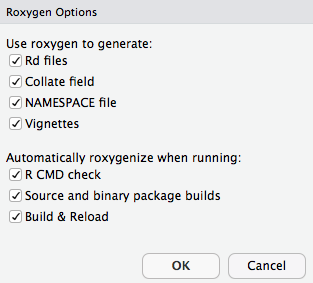
\includegraphics[width=4.35in]{images/ch3_configure_build_tools} 

}

\caption{Roxygen options}\label{fig:pkg8}
\end{figure}

\subsection{\texorpdfstring{\texttt{man}
page}{man page}}\label{man-page}

File `\texttt{man/linmodEst.Rd} contains:

\begin{Shaded}
\begin{Highlighting}[]
\NormalTok{% Generated by roxygen2}\OperatorTok{:}\StringTok{ }\NormalTok{do not edit by hand}
\NormalTok{% Please edit documentation }\ControlFlowTok{in}\NormalTok{ R}\OperatorTok{/}\NormalTok{linreg.R}
\NormalTok{\textbackslash{}name\{linmodEst\}}
\NormalTok{\textbackslash{}alias\{linmodEst\}}
\NormalTok{\textbackslash{}title\{Linear regression\}}
\NormalTok{\textbackslash{}usage\{}
\KeywordTok{linmodEst}\NormalTok{(x, y)}
\NormalTok{\}}
\NormalTok{\textbackslash{}arguments\{}
\NormalTok{\textbackslash{}item\{y\}\{response }\KeywordTok{vector}\NormalTok{ (}\DecValTok{1}\NormalTok{ x n)\}}

\NormalTok{\textbackslash{}item\{X\}\{covariate }\KeywordTok{matrix}\NormalTok{ (p x n) with no intercept\}}
\NormalTok{\}}
\NormalTok{\textbackslash{}value\{}
\NormalTok{A list with }\DecValTok{4}\NormalTok{ elements}\OperatorTok{:}\StringTok{ }\NormalTok{coefficients, vcov, sigma, df}
\NormalTok{\}}
\NormalTok{\textbackslash{}description\{}
\NormalTok{Runs an OLS regression not unlike \textbackslash{}code\{\textbackslash{}link\{lm\}\}}
\NormalTok{\}}
\NormalTok{\textbackslash{}examples\{}
\KeywordTok{data}\NormalTok{(mtcars)}
\NormalTok{X <-}\StringTok{ }\KeywordTok{as.matrix}\NormalTok{(mtcars[, }\KeywordTok{c}\NormalTok{(}\StringTok{"cyl"}\NormalTok{, }\StringTok{"disp"}\NormalTok{, }\StringTok{"hp"}\NormalTok{)])}
\NormalTok{y <-}\StringTok{ }\NormalTok{mtcars[, }\StringTok{"mpg"}\NormalTok{]}
\KeywordTok{linmodEst}\NormalTok{(y, X)}

\NormalTok{\}}
\end{Highlighting}
\end{Shaded}

\subsection{Formatted output}\label{formatted-output}

\begin{figure}

{\centering 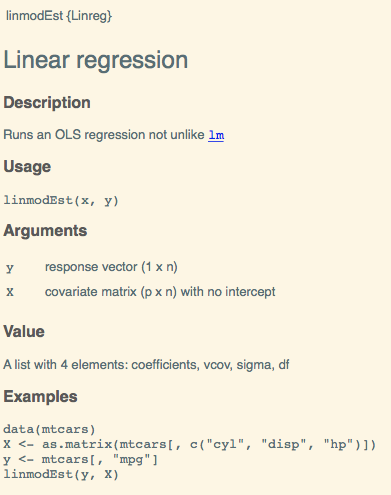
\includegraphics[width=5.43in]{images/ch3_formatted_help} 

}

\end{figure}

\subsection{\texorpdfstring{\texttt{DESCRIPTION}}{DESCRIPTION}}\label{description}

Reading: \url{http://r-pkgs.had.co.nz/description.html}

\begin{Shaded}
\begin{Highlighting}[]
\NormalTok{Package}\OperatorTok{:}\StringTok{ }\NormalTok{Linreg}
\NormalTok{Type}\OperatorTok{:}\StringTok{ }\NormalTok{Package}
\NormalTok{Title}\OperatorTok{:}\StringTok{ }\NormalTok{What the Package }\KeywordTok{Does}\NormalTok{ (Title Case)}
\NormalTok{Version}\OperatorTok{:}\StringTok{ }\FloatTok{0.1}\NormalTok{.}\DecValTok{0}
\NormalTok{Author}\OperatorTok{:}\StringTok{ }\NormalTok{Who wrote it}
\NormalTok{Maintainer}\OperatorTok{:}\StringTok{ }\NormalTok{The package maintainer }\OperatorTok{<}\NormalTok{yourself}\OperatorTok{@}\NormalTok{somewhere.net}\OperatorTok{>}
\NormalTok{Description}\OperatorTok{:}\StringTok{ }\NormalTok{More about what it }\KeywordTok{does}\NormalTok{ (maybe more than one line)}
\NormalTok{    Use four spaces when indenting paragraphs within the Description.}
\NormalTok{License}\OperatorTok{:}\StringTok{ }\NormalTok{What license is it under?}
\NormalTok{Encoding}\OperatorTok{:}\StringTok{ }\NormalTok{UTF}\OperatorTok{-}\DecValTok{8}
\NormalTok{LazyData}\OperatorTok{:}\StringTok{ }\NormalTok{true}
\NormalTok{RoxygenNote}\OperatorTok{:}\StringTok{ }\FloatTok{6.0}\NormalTok{.}\DecValTok{1}
\end{Highlighting}
\end{Shaded}

\subsection{\texorpdfstring{\texttt{NAMESPACE}}{NAMESPACE}}\label{namespace}

Reading: \url{http://r-pkgs.had.co.nz/namespace.html}, in particular
\texttt{Imports} vs \texttt{Suggests}

\texttt{export}'s automatically generated when parsing ROxygen2 snippets

\begin{Shaded}
\begin{Highlighting}[]
\KeywordTok{export}\NormalTok{(linmodEst)}
\end{Highlighting}
\end{Shaded}

\begin{figure}

{\centering 
\includegraphics[width=6.86in]{images/ch3_pumpkin} 

}

\end{figure}

\begin{figure}

{\centering 
\includegraphics[width=12.44in]{images/ch3_octocat-de-los-muertos} 

}

\end{figure}

\begin{itemize}
\item
  A scary hack
\item
  A scary tree
\end{itemize}

Reading:
\url{https://git-scm.com/book/en/v2/Git-Branching-Basic-Branching-and-Merging}

\begin{figure}

{\centering 
\includegraphics[width=14.56in]{images/ch3_halloween_tree} 

}

\end{figure}

\subsection{S3 basics}\label{s3-basics}

Reading: \url{http://adv-r.had.co.nz/S3.html}

\begin{Shaded}
\begin{Highlighting}[]
\NormalTok{hello <-}\StringTok{ }\ControlFlowTok{function}\NormalTok{() \{}
\NormalTok{ s <-}\StringTok{ "Hello World!"}
 \KeywordTok{class}\NormalTok{(s) <-}\StringTok{ "hi"}
 \KeywordTok{return}\NormalTok{(s)}
\NormalTok{\}}

\KeywordTok{hello}\NormalTok{()}
\end{Highlighting}
\end{Shaded}

\begin{verbatim}
## [1] "Hello World!"
## attr(,"class")
## [1] "hi"
\end{verbatim}

\begin{Shaded}
\begin{Highlighting}[]
\NormalTok{print.hi <-}\StringTok{ }\ControlFlowTok{function}\NormalTok{(...) \{}
  \KeywordTok{print}\NormalTok{(}\StringTok{"Surprise!"}\NormalTok{)}
\NormalTok{\}}

\KeywordTok{hello}\NormalTok{()}
\end{Highlighting}
\end{Shaded}

\begin{verbatim}
## [1] "Surprise!"
\end{verbatim}

\subsection{S3 and S4 generics}\label{s3-and-s4-generics}

Reading: \url{http://adv-r.had.co.nz/S4.html}

\begin{Shaded}
\begin{Highlighting}[]
\NormalTok{linmod <-}\StringTok{ }\ControlFlowTok{function}\NormalTok{(x, ...)}
  \KeywordTok{UseMethod}\NormalTok{(}\StringTok{"linmod"}\NormalTok{)}
\end{Highlighting}
\end{Shaded}

\begin{Shaded}
\begin{Highlighting}[]
\NormalTok{linmod.default <-}\StringTok{ }\ControlFlowTok{function}\NormalTok{(x, y, ...) \{}
\NormalTok{  x <-}\StringTok{ }\KeywordTok{as.matrix}\NormalTok{(x)}
\NormalTok{  y <-}\StringTok{ }\KeywordTok{as.numeric}\NormalTok{(y)}
\NormalTok{  est <-}\StringTok{ }\KeywordTok{linmodEst}\NormalTok{(x, y)}
\NormalTok{  est}\OperatorTok{$}\NormalTok{fitted.values <-}\StringTok{ }\KeywordTok{as.vector}\NormalTok{(x }\OperatorTok\StringTok{ }\NormalTok{est}\OperatorTok{$}\NormalTok{coefficients)}
\NormalTok{  est}\OperatorTok{$}\NormalTok{residuals <-}\StringTok{ }\NormalTok{y }\OperatorTok{-}\StringTok{ }\NormalTok{est}\OperatorTok{$}\NormalTok{fitted.values}
\NormalTok{  est}\OperatorTok{$}\NormalTok{call <-}\StringTok{ }\KeywordTok{match.call}\NormalTok{()}
  \KeywordTok{class}\NormalTok{(est) <-}\StringTok{ "linmod"}
  \KeywordTok{return}\NormalTok{(est)}
\NormalTok{\}}
\end{Highlighting}
\end{Shaded}

\subsection{\texorpdfstring{\texttt{print}}{print}}\label{print}

\begin{Shaded}
\begin{Highlighting}[]
\NormalTok{print.linmod <-}\StringTok{ }\ControlFlowTok{function}\NormalTok{(x, ...) \{}
  \KeywordTok{cat}\NormalTok{(}\StringTok{"Call:}\CharTok{\textbackslash{}n}\StringTok{"}\NormalTok{)}
  \KeywordTok{print}\NormalTok{(x}\OperatorTok{$}\NormalTok{call)}
  \KeywordTok{cat}\NormalTok{(}\StringTok{"}\CharTok{\textbackslash{}n}\StringTok{Coefficients:}\CharTok{\textbackslash{}n}\StringTok{"}\NormalTok{)}
  \KeywordTok{print}\NormalTok{(x}\OperatorTok{$}\NormalTok{coefficients)}
\NormalTok{\}}
\end{Highlighting}
\end{Shaded}

\begin{Shaded}
\begin{Highlighting}[]
\NormalTok{x <-}\StringTok{ }\KeywordTok{cbind}\NormalTok{(}\DataTypeTok{Const =} \DecValTok{1}\NormalTok{, }\DataTypeTok{Bwt =}\NormalTok{ cats}\OperatorTok{$}\NormalTok{Bwt)}
\NormalTok{y <-}\StringTok{ }\NormalTok{cats}\OperatorTok{$}\NormalTok{Hw}
\NormalTok{mod1 <-}\StringTok{ }\KeywordTok{linmod}\NormalTok{(x, y)}
\end{Highlighting}
\end{Shaded}

\begin{verbatim}
##             [,1]
## Const -0.3566624
## Bwt    4.0340627
\end{verbatim}

\begin{Shaded}
\begin{Highlighting}[]
\NormalTok{mod1}
\end{Highlighting}
\end{Shaded}

\begin{verbatim}
## Call:
## linmod.default(x = x, y = y)
## 
## Coefficients:
##             [,1]
## Const -0.3566624
## Bwt    4.0340627
\end{verbatim}

\subsection{Other methods}\label{other-methods}

\begin{itemize}
\item
  \texttt{summary.linmod}
\item
  \texttt{print.summary.linmod}
\item
  \texttt{predict.linmod}
\item
  \texttt{plot.linmod}
\item
  \texttt{coef.linmod}, \texttt{vcov.linmod}, \ldots{}
\end{itemize}

\BeginKnitrBlock{exercise}
\protect\hypertarget{exr:unnamed-chunk-47}{}{\label{exr:unnamed-chunk-47}
}Write two functions that implement the \texttt{coef.linmod} and
\texttt{vcov.linmod} methods.
\EndKnitrBlock{exercise}

\subsection{Formulas and model frames}\label{formulas-and-model-frames}

Reading:
\url{http://genomicsclass.github.io/book/pages/expressing_design_formula.html}

\begin{quote}
\texttt{model.frame} (a generic function) and its methods return a
data.frame with the variables needed to use formula and any \ldots{}
arguments.
\end{quote}

\begin{quote}
\texttt{model.matrix} creates a design (or model) matrix, e.g., by
expanding factors to a set of dummy variables (depending on the
contrasts) and expanding interactions similarly.
\end{quote}

\begin{quote}
\texttt{model.response} returns the response of a model frame passed as
optional arguments to model.frame.
\end{quote}

\BeginKnitrBlock{exercise}
\protect\hypertarget{exr:unnamed-chunk-48}{}{\label{exr:unnamed-chunk-48}
}What is \texttt{model.extract}?
\EndKnitrBlock{exercise}

\begin{Shaded}
\begin{Highlighting}[]
\NormalTok{linmod.formula <-}\StringTok{ }\ControlFlowTok{function}\NormalTok{(formula, }\DataTypeTok{data =} \KeywordTok{list}\NormalTok{(), ...) \{}
\NormalTok{  mf <-}\StringTok{ }\KeywordTok{model.frame}\NormalTok{(}\DataTypeTok{formula =}\NormalTok{ formula, }\DataTypeTok{data =}\NormalTok{ data)}
\NormalTok{  x <-}\StringTok{ }\KeywordTok{model.matrix}\NormalTok{(}\KeywordTok{attr}\NormalTok{(mf, }\StringTok{"terms"}\NormalTok{), }\DataTypeTok{data =}\NormalTok{ mf)}
\NormalTok{  y <-}\StringTok{ }\KeywordTok{model.response}\NormalTok{(mf)}
\NormalTok{  est <-}\StringTok{ }\KeywordTok{linmod.default}\NormalTok{(x, y, ...)}
\NormalTok{  est}\OperatorTok{$}\NormalTok{call <-}\StringTok{ }\KeywordTok{match.call}\NormalTok{()}
\NormalTok{  est}\OperatorTok{$}\NormalTok{formula <-}\StringTok{ }\NormalTok{formula}
  \KeywordTok{return}\NormalTok{(est)}
\NormalTok{\}}
\end{Highlighting}
\end{Shaded}

\begin{Shaded}
\begin{Highlighting}[]
\KeywordTok{linmod}\NormalTok{(Hwt }\OperatorTok{~}\StringTok{ }\OperatorTok{-}\StringTok{ }\DecValTok{1} \OperatorTok{+}\StringTok{ }\NormalTok{Bwt }\OperatorTok{*}\StringTok{ }\NormalTok{Sex, }\DataTypeTok{data =}\NormalTok{ cats)}
\end{Highlighting}
\end{Shaded}

\begin{Shaded}
\begin{Highlighting}[]
\NormalTok{Call}\OperatorTok{:}
\KeywordTok{linmod.formula}\NormalTok{(}\DataTypeTok{formula =}\NormalTok{ Hwt }\OperatorTok{~}\StringTok{ }\OperatorTok{-}\DecValTok{1} \OperatorTok{+}\StringTok{ }\NormalTok{Bwt }\OperatorTok{*}\StringTok{ }\NormalTok{Sex, }\DataTypeTok{data =}\NormalTok{ cats)}

\NormalTok{Coefficients}\OperatorTok{:}
\StringTok{      }\NormalTok{Bwt      SexF      SexM  Bwt}\OperatorTok{:}\NormalTok{SexM }
 \FloatTok{2.636414}  \FloatTok{2.981312} \OperatorTok{-}\FloatTok{1.184088}  \FloatTok{1.676265} 
\end{Highlighting}
\end{Shaded}

\section{Unit testing}\label{unit-testing}

\subsection{\texorpdfstring{Unit tests and
\texttt{testthat}}{Unit tests and testthat}}\label{unit-tests-and-testthat}

Reading: \url{http://r-pkgs.had.co.nz/tests.html}

In package directory:

\begin{Shaded}
\begin{Highlighting}[]
\NormalTok{devtools}\OperatorTok{::}\KeywordTok{use_testthat}\NormalTok{()}
\end{Highlighting}
\end{Shaded}

pre-populates \texttt{test/testthat/}

Test files should start with \texttt{test} to be processed.

\subsection{\texorpdfstring{\texttt{test\_coef.R}}{test\_coef.R}}\label{test_coef.r}

\begin{Shaded}
\begin{Highlighting}[]
\KeywordTok{data}\NormalTok{(cats, }\DataTypeTok{package =} \StringTok{"MASS"}\NormalTok{)}
\NormalTok{l1 <-}\StringTok{ }\KeywordTok{linmod}\NormalTok{(Hwt }\OperatorTok{~}\StringTok{ }\NormalTok{Bwt }\OperatorTok{*}\StringTok{ }\NormalTok{Sex, }\DataTypeTok{data =}\NormalTok{ cats)}
\NormalTok{l2 <-}\StringTok{ }\KeywordTok{lm}\NormalTok{(Hwt }\OperatorTok{~}\StringTok{ }\NormalTok{Bwt }\OperatorTok{*}\StringTok{ }\NormalTok{Sex, }\DataTypeTok{data =}\NormalTok{ cats)}

\KeywordTok{test_that}\NormalTok{(}\StringTok{"same estimated coefficients as lm function"}\NormalTok{, \{}
  \KeywordTok{expect_equal}\NormalTok{(}\KeywordTok{round}\NormalTok{(l1}\OperatorTok{$}\NormalTok{coefficients, }\DecValTok{3}\NormalTok{), }\KeywordTok{round}\NormalTok{(l2}\OperatorTok{$}\NormalTok{coefficients, }\DecValTok{3}\NormalTok{))}
\NormalTok{\})}
\end{Highlighting}
\end{Shaded}

\begin{Shaded}
\begin{Highlighting}[]
\OperatorTok{>}\StringTok{ }\NormalTok{devtools}\OperatorTok{::}\KeywordTok{test}\NormalTok{()}
\NormalTok{Loading Linreg}
\NormalTok{Loading required package}\OperatorTok{:}\StringTok{ }\NormalTok{testthat}
\NormalTok{Testing Linreg}
\NormalTok{.}
\NormalTok{DONE }\OperatorTok{==}\ErrorTok{=======================================================================================}
\end{Highlighting}
\end{Shaded}

\section{Continuous integration}\label{continuous-integration}

Readings: - \url{http://r-pkgs.had.co.nz/check.html\#travis} -
\url{https://juliasilge.com/blog/beginners-guide-to-travis/}

Website: \url{https://travis-ci.org/}

First step is to create a Travis account and link it to you GitHub
account.

\begin{figure}

{\centering 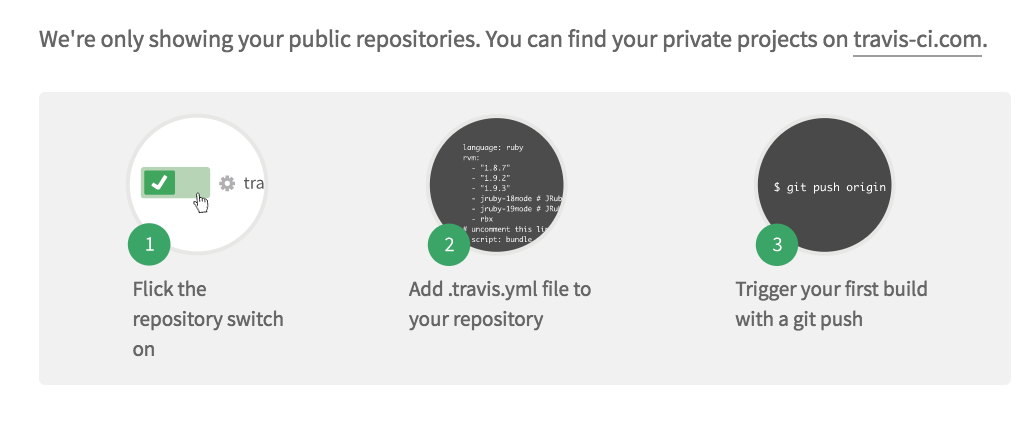
\includegraphics[width=14.38in]{images/ch3_travis_github} 

}

\end{figure}

Travis will list all your public GitHub repositories for you to select
the ones you want to test.

\begin{figure}

{\centering 
\includegraphics[width=5.39in]{images/ch3_travis_Linreg} 

}

\end{figure}

Calling

\begin{Shaded}
\begin{Highlighting}[]
\NormalTok{devtools}\OperatorTok{::}\KeywordTok{use_coverage}\NormalTok{(}\DataTypeTok{pkg =} \StringTok{"."}\NormalTok{, }\DataTypeTok{type =} \KeywordTok{c}\NormalTok{(}\StringTok{"codecov"}\NormalTok{))}
\end{Highlighting}
\end{Shaded}

creates the \texttt{.travis.yml} file:

\begin{Shaded}
\begin{Highlighting}[]
\CommentTok{# R for travis: see documentation at https://docs.travis-ci.com/user/languages/r}

\NormalTok{language}\OperatorTok{:}\StringTok{ }\NormalTok{R}
\NormalTok{sudo}\OperatorTok{:}\StringTok{ }\NormalTok{false}
\NormalTok{cache}\OperatorTok{:}\StringTok{ }\NormalTok{packages}
\end{Highlighting}
\end{Shaded}

and pushing \texttt{Linreg} code to GitHub will automatically triggers a
Travis build\ldots{} which fails!

\begin{figure}

{\centering 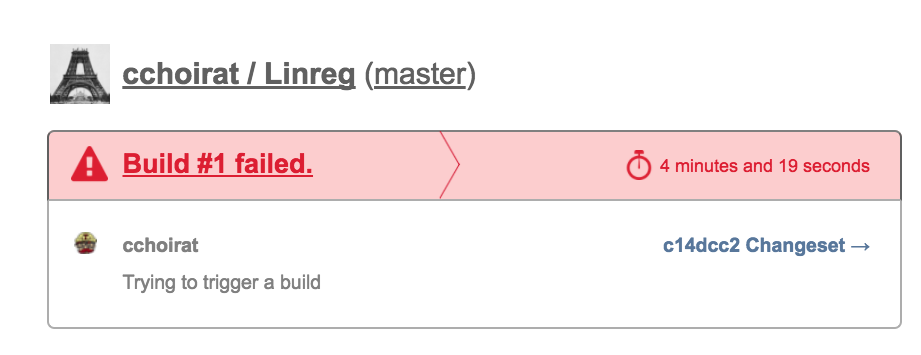
\includegraphics[width=12.79in]{images/ch3_travis_failed_build} 

}

\end{figure}

To be continued\ldots{}

\section{Code coverage}\label{code-coverage}

Reading:
\url{https://walczak.org/2017/06/how-to-add-code-coverage-codecov-to-your-r-package/}

Website: \url{https://codecov.io/}

Like Travis, codecov has to be linked to a GitHub account:

\begin{figure}

{\centering 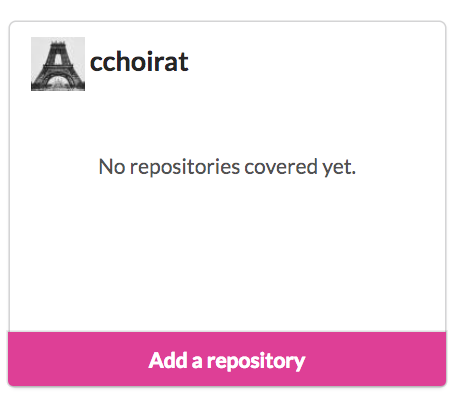
\includegraphics[width=6.38in]{images/ch3_codecov_github} 

}

\end{figure}

\begin{Shaded}
\begin{Highlighting}[]
\NormalTok{devtools}\OperatorTok{::}\KeywordTok{use_coverage}\NormalTok{(}\DataTypeTok{pkg =} \StringTok{"."}\NormalTok{, }\DataTypeTok{type =} \KeywordTok{c}\NormalTok{(}\StringTok{"codecov"}\NormalTok{))}
\end{Highlighting}
\end{Shaded}

creates the \texttt{codecov.yml} file:

\begin{Shaded}
\begin{Highlighting}[]
\NormalTok{comment}\OperatorTok{:}\StringTok{ }\NormalTok{false}
\end{Highlighting}
\end{Shaded}

A call to

\begin{Shaded}
\begin{Highlighting}[]
\NormalTok{covr}\OperatorTok{::}\KeywordTok{codecov}\NormalTok{(}\DataTypeTok{token =} \StringTok{"YOUR_TOKEN"}\NormalTok{)}
\end{Highlighting}
\end{Shaded}

will give you code coverage information:

\begin{figure}

{\centering 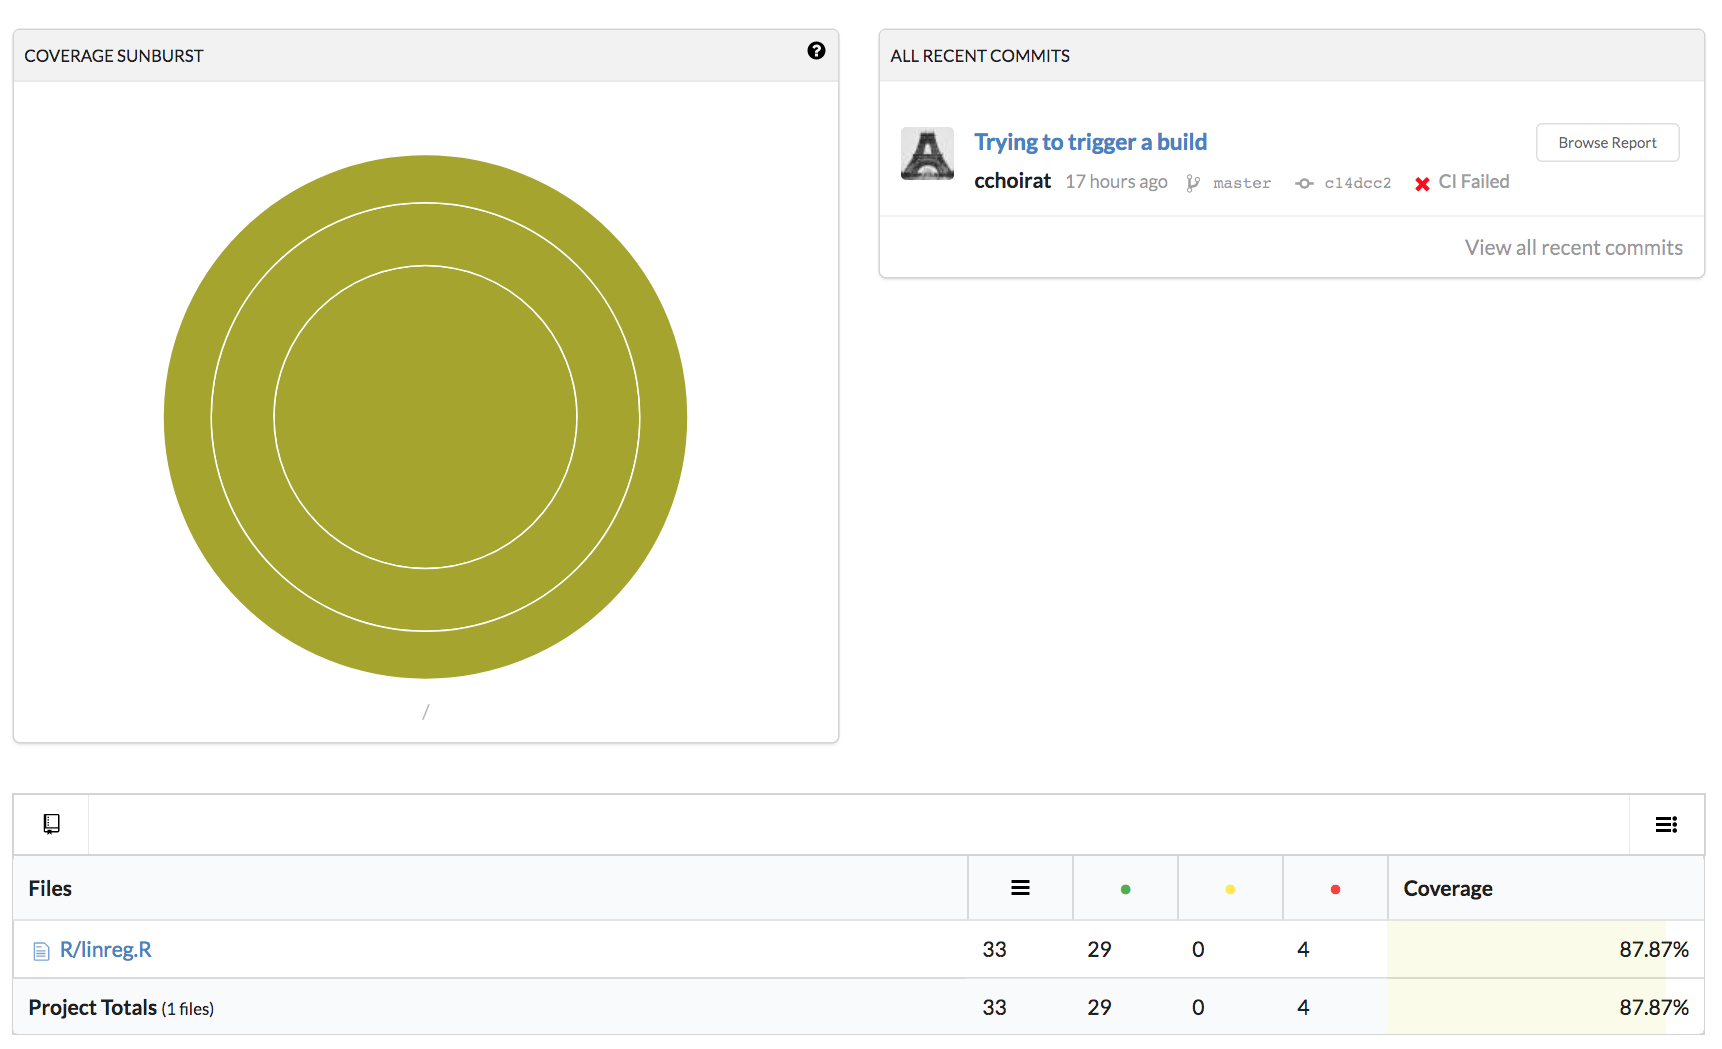
\includegraphics[width=23.92in]{images/ch3_codecov_out} 

}

\end{figure}

\section{Back to GitHub}\label{back-to-github}

Badges can be added to \texttt{README.md}:

\begin{Shaded}
\begin{Highlighting}[]
\OperatorTok{<!---}\StringTok{ }\NormalTok{Badges }\OperatorTok{----}\NormalTok{->}
\NormalTok{[}\OperatorTok{!}\NormalTok{[}\KeywordTok{Travis}\NormalTok{ (LINUX) Build Status](https}\OperatorTok{:}\ErrorTok{//}\NormalTok{travis}\OperatorTok{-}\NormalTok{ci.org}\OperatorTok{/}\NormalTok{cchoirat}\OperatorTok{/}\NormalTok{Linreg.svg?}\DataTypeTok{branch=}\NormalTok{master)](https}\OperatorTok{:}\ErrorTok{//}\NormalTok{travis}\OperatorTok{-}\NormalTok{ci.org}\OperatorTok{/}\NormalTok{cchoirat}\OperatorTok{/}\NormalTok{Linreg)}
\NormalTok{[}\OperatorTok{!}\NormalTok{[codecov](https}\OperatorTok{:}\ErrorTok{//}\NormalTok{codecov.io}\OperatorTok{/}\NormalTok{gh}\OperatorTok{/}\NormalTok{cchoirat}\OperatorTok{/}\NormalTok{Linreg}\OperatorTok{/}\NormalTok{branch}\OperatorTok{/}\NormalTok{master}\OperatorTok{/}\NormalTok{graph}\OperatorTok{/}\NormalTok{badge.svg)](https}\OperatorTok{:}\ErrorTok{//}\NormalTok{codecov.io}\OperatorTok{/}\NormalTok{gh}\OperatorTok{/}\NormalTok{cchoirat}\OperatorTok{/}\NormalTok{Linreg)}

\NormalTok{## `Linreg` package template}

\NormalTok{Based on }\StringTok{"Creating R Packages: A Tutorial"}\NormalTok{ (Friedrich Leisch, }\DecValTok{2009}\NormalTok{)}

\OperatorTok{-}\StringTok{ }\NormalTok{https}\OperatorTok{:}\ErrorTok{//}\NormalTok{cran.r}\OperatorTok{-}\NormalTok{project.org}\OperatorTok{/}\NormalTok{doc}\OperatorTok{/}\NormalTok{contrib}\OperatorTok{/}\NormalTok{Leisch}\OperatorTok{-}\NormalTok{CreatingPackages.pdf}
\end{Highlighting}
\end{Shaded}

are automatically displayed on GitHub:

\begin{figure}

{\centering 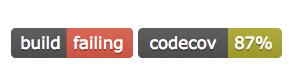
\includegraphics[width=4.06in]{images/ch3_badges} 

}

\end{figure}

\section{Vignettes}\label{vignettes}

Reading: \url{http://r-pkgs.had.co.nz/vignettes.html}

Reading: \url{http://kbroman.org/pkg_primer/pages/vignettes.html}

Even if all the functions and datasets of your package are documented,
it is still useful to have a more detailed illustation on how to use
your package. A \emph{vignette} is the right place to explain a worflow
and a statistical method.

Running:

\begin{Shaded}
\begin{Highlighting}[]
\NormalTok{devtools}\OperatorTok{::}\KeywordTok{use_vignette}\NormalTok{(}\StringTok{"my-linear-regression"}\NormalTok{)}
\end{Highlighting}
\end{Shaded}

creates a \texttt{vignettes} folder and provide a template in RMarkdown
format \texttt{my-linear-regression.Rmd}:

\url{https://github.com/cchoirat/Linreg/blob/master/vignettes/my-linear-regression.Rmd}

It also indicates in \texttt{DESCRIPTION} that vignettes should be built
with \texttt{knitr}.

\begin{Shaded}
\begin{Highlighting}[]
\NormalTok{VignetteBuilder}\OperatorTok{:}\StringTok{ }\NormalTok{knitr}
\end{Highlighting}
\end{Shaded}

The vignette is built into a HTML document with

\begin{Shaded}
\begin{Highlighting}[]
\NormalTok{devtools}\OperatorTok{::}\KeywordTok{build_vignettes}\NormalTok{()}
\end{Highlighting}
\end{Shaded}

\begin{Shaded}
\begin{Highlighting}[]
\NormalTok{Building Linreg vignettes}
\NormalTok{Moving my}\OperatorTok{-}\NormalTok{linear}\OperatorTok{-}\NormalTok{regression.html, my}\OperatorTok{-}\NormalTok{linear}\OperatorTok{-}\NormalTok{regression.R to inst}\OperatorTok{/}\NormalTok{doc}\OperatorTok{/}
\NormalTok{Copying my}\OperatorTok{-}\NormalTok{linear}\OperatorTok{-}\NormalTok{regression.Rmd to inst}\OperatorTok{/}\NormalTok{doc}\OperatorTok{/}
\end{Highlighting}
\end{Shaded}

The vignette is accessible with

\begin{Shaded}
\begin{Highlighting}[]
\KeywordTok{vignette}\NormalTok{(}\StringTok{"my-linear-regression"}\NormalTok{)}
\KeywordTok{vignette}\NormalTok{(}\StringTok{"my-linear-regression"}\NormalTok{, }\DataTypeTok{package =} \StringTok{"Linreg"}\NormalTok{)}
\end{Highlighting}
\end{Shaded}

\begin{figure}

{\centering 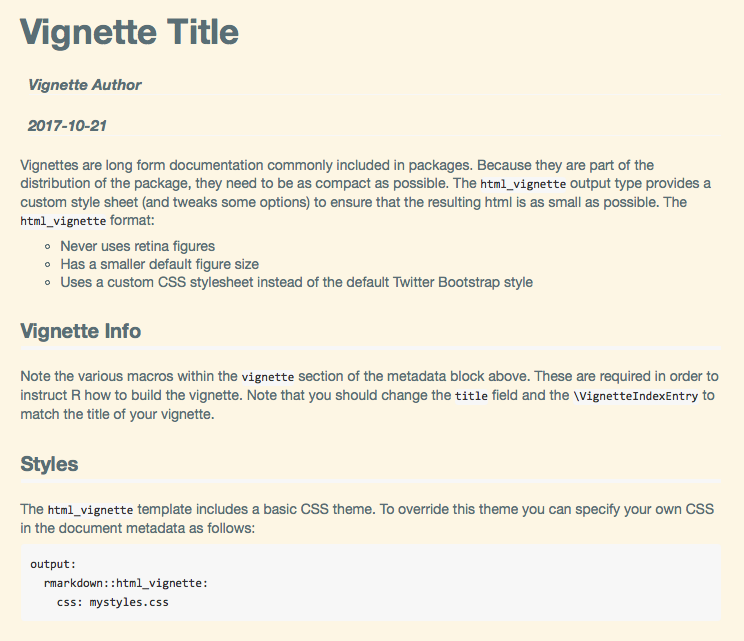
\includegraphics[width=10.33in]{images/ch3_vignette_html} 

}

\end{figure}

\chapter{Optimization}\label{optimization}

In this Chapter, we will see how to measure and improve code
performance.

\section{Measuring performance}\label{measuring-performance}

\subsection{Benchmarking}\label{benchmarking}

Reading:
\url{http://adv-r.had.co.nz/Performance.html\#microbenchmarking}

There are several ways to benchmark code (see
\url{http://www.alexejgossmann.com/benchmarking_r/}) from
\texttt{system.time} to dedicated packages such as \texttt{rbenchmark}
(\citet{rbenchmark}) or \texttt{microbenchmark}
(\citet{microbenchmark}).

Let's start with an example from \citet{Wickham2014}.

\begin{Shaded}
\begin{Highlighting}[]
\KeywordTok{library}\NormalTok{(microbenchmark)}
\NormalTok{m <-}\StringTok{ }\KeywordTok{microbenchmark}\NormalTok{(}
  \DataTypeTok{times =} \DecValTok{1000}\NormalTok{, }\CommentTok{# default is 100}
  \StringTok{"[32, 11]"}\NormalTok{      =}\StringTok{ }\NormalTok{mtcars[}\DecValTok{32}\NormalTok{, }\DecValTok{11}\NormalTok{],}
  \StringTok{"$carb[32]"}\NormalTok{     =}\StringTok{ }\NormalTok{mtcars}\OperatorTok{$}\NormalTok{carb[}\DecValTok{32}\NormalTok{],}
  \StringTok{"[[c(11, 32)]]"}\NormalTok{ =}\StringTok{ }\NormalTok{mtcars[[}\KeywordTok{c}\NormalTok{(}\DecValTok{11}\NormalTok{, }\DecValTok{32}\NormalTok{)]],}
  \StringTok{"[[11]][32]"}\NormalTok{    =}\StringTok{ }\NormalTok{mtcars[[}\DecValTok{11}\NormalTok{]][}\DecValTok{32}\NormalTok{],}
  \StringTok{".subset2"}\NormalTok{      =}\StringTok{ }\KeywordTok{.subset2}\NormalTok{(mtcars, }\DecValTok{11}\NormalTok{)[}\DecValTok{32}\NormalTok{]}
\NormalTok{)}
\NormalTok{m}
\end{Highlighting}
\end{Shaded}

\begin{verbatim}
## Unit: nanoseconds
##           expr  min      lq      mean  median      uq   max neval
##       [32, 11] 8783 10046.0 11326.018 10673.5 11362.5 73789  1000
##      $carb[32] 4536  5697.5  6763.718  6214.0  6865.0 50683  1000
##  [[c(11, 32)]] 3732  4628.5  5377.422  5029.5  5507.0 33802  1000
##     [[11]][32] 3467  4287.5  5093.947  4712.5  5166.5 45145  1000
##       .subset2  207   275.0   378.369   323.0   394.5 16201  1000
\end{verbatim}

\begin{Shaded}
\begin{Highlighting}[]
\NormalTok{ggplot2}\OperatorTok{::}\KeywordTok{autoplot}\NormalTok{(m)}
\end{Highlighting}
\end{Shaded}

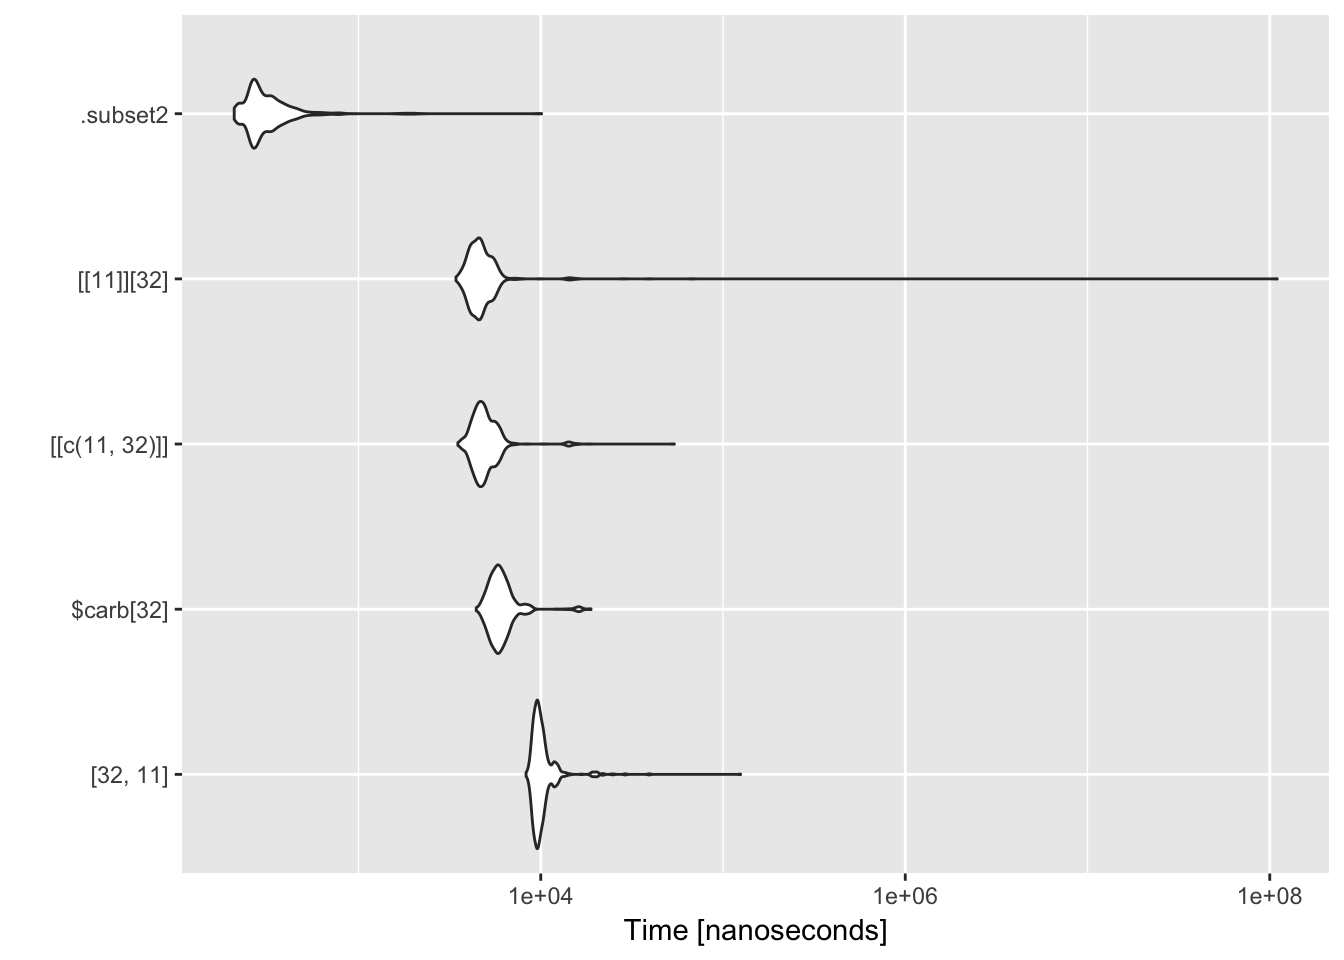
\includegraphics{Computing_for_Big_Data_files/figure-latex/unnamed-chunk-67-1.pdf}

\subsection{Profiling and
optimization}\label{profiling-and-optimization}

Reading: \url{http://adv-r.had.co.nz/Profiling.html\#measure-perf}

Let's compare three ways of estimating a linear regression: with
built-in \texttt{lm} and with two functions we defined in package
\texttt{Linreg} in Chapter \ref{packages}.

\begin{Shaded}
\begin{Highlighting}[]
\KeywordTok{library}\NormalTok{(Linreg)}
\KeywordTok{data}\NormalTok{(cats, }\DataTypeTok{package =} \StringTok{"MASS"}\NormalTok{)}
\NormalTok{fit1 <-}\StringTok{ }\KeywordTok{lm}\NormalTok{(Hwt }\OperatorTok{~}\StringTok{ }\NormalTok{Bwt, }\DataTypeTok{data =}\NormalTok{ cats)}
\NormalTok{fit2 <-}\StringTok{ }\KeywordTok{linmod}\NormalTok{(Hwt }\OperatorTok{~}\StringTok{ }\NormalTok{Bwt, }\DataTypeTok{data =}\NormalTok{ cats)}
\NormalTok{fit3 <-}\StringTok{ }\KeywordTok{linmodEst}\NormalTok{(}\KeywordTok{cbind}\NormalTok{(}\DecValTok{1}\NormalTok{, cats}\OperatorTok{$}\NormalTok{Bwt), cats}\OperatorTok{$}\NormalTok{Hwt)}
\end{Highlighting}
\end{Shaded}

\begin{verbatim}
##            [,1]
## [1,] -0.3566624
## [2,]  4.0340627
\end{verbatim}

\begin{Shaded}
\begin{Highlighting}[]
\KeywordTok{all.equal}\NormalTok{(}\KeywordTok{round}\NormalTok{(}\KeywordTok{coef}\NormalTok{(fit1), }\DecValTok{5}\NormalTok{), }\KeywordTok{round}\NormalTok{(}\KeywordTok{coef}\NormalTok{(fit2), }\DecValTok{5}\NormalTok{))}
\end{Highlighting}
\end{Shaded}

\begin{verbatim}
## [1] "names for target but not for current"                             
## [2] "Attributes: < names for current but not for target >"             
## [3] "Attributes: < Length mismatch: comparison on first 0 components >"
## [4] "target is numeric, current is matrix"
\end{verbatim}

\begin{Shaded}
\begin{Highlighting}[]
\KeywordTok{all.equal}\NormalTok{(}\KeywordTok{round}\NormalTok{(}\KeywordTok{coef}\NormalTok{(fit1), }\DecValTok{5}\NormalTok{), }\KeywordTok{round}\NormalTok{(fit3}\OperatorTok{$}\NormalTok{coefficients, }\DecValTok{5}\NormalTok{), }\DataTypeTok{check.names =} \OtherTok{FALSE}\NormalTok{)}
\end{Highlighting}
\end{Shaded}

\begin{verbatim}
## [1] "Attributes: < names for current but not for target >"             
## [2] "Attributes: < Length mismatch: comparison on first 0 components >"
## [3] "target is numeric, current is matrix"
\end{verbatim}

\begin{Shaded}
\begin{Highlighting}[]
\NormalTok{m <-}\StringTok{ }\KeywordTok{microbenchmark}\NormalTok{(}
\NormalTok{  fit1 <-}\StringTok{ }\KeywordTok{lm}\NormalTok{(Hwt }\OperatorTok{~}\StringTok{ }\NormalTok{Bwt, }\DataTypeTok{data =}\NormalTok{ cats),}
\NormalTok{  fit2 <-}\StringTok{ }\KeywordTok{linmod}\NormalTok{(Hwt }\OperatorTok{~}\StringTok{ }\NormalTok{Bwt, }\DataTypeTok{data =}\NormalTok{ cats),}
\NormalTok{  fit3 <-}\StringTok{ }\KeywordTok{linmodEst}\NormalTok{(}\KeywordTok{cbind}\NormalTok{(}\DecValTok{1}\NormalTok{, cats}\OperatorTok{$}\NormalTok{Bwt), cats}\OperatorTok{$}\NormalTok{Hwt)}
  \CommentTok{# custom checks can be performed with the 'check' argument}
\NormalTok{)}
\end{Highlighting}
\end{Shaded}

\begin{verbatim}
##            [,1]
## [1,] -0.3566624
## [2,]  4.0340627
##            [,1]
## [1,] -0.3566624
## [2,]  4.0340627
##            [,1]
## [1,] -0.3566624
## [2,]  4.0340627
##            [,1]
## [1,] -0.3566624
## [2,]  4.0340627
##            [,1]
## [1,] -0.3566624
## [2,]  4.0340627
##            [,1]
## [1,] -0.3566624
## [2,]  4.0340627
##            [,1]
## [1,] -0.3566624
## [2,]  4.0340627
##            [,1]
## [1,] -0.3566624
## [2,]  4.0340627
##            [,1]
## [1,] -0.3566624
## [2,]  4.0340627
##            [,1]
## [1,] -0.3566624
## [2,]  4.0340627
##            [,1]
## [1,] -0.3566624
## [2,]  4.0340627
##            [,1]
## [1,] -0.3566624
## [2,]  4.0340627
##            [,1]
## [1,] -0.3566624
## [2,]  4.0340627
##            [,1]
## [1,] -0.3566624
## [2,]  4.0340627
##            [,1]
## [1,] -0.3566624
## [2,]  4.0340627
##            [,1]
## [1,] -0.3566624
## [2,]  4.0340627
##            [,1]
## [1,] -0.3566624
## [2,]  4.0340627
##            [,1]
## [1,] -0.3566624
## [2,]  4.0340627
##            [,1]
## [1,] -0.3566624
## [2,]  4.0340627
##            [,1]
## [1,] -0.3566624
## [2,]  4.0340627
##            [,1]
## [1,] -0.3566624
## [2,]  4.0340627
##            [,1]
## [1,] -0.3566624
## [2,]  4.0340627
##            [,1]
## [1,] -0.3566624
## [2,]  4.0340627
##            [,1]
## [1,] -0.3566624
## [2,]  4.0340627
##            [,1]
## [1,] -0.3566624
## [2,]  4.0340627
##            [,1]
## [1,] -0.3566624
## [2,]  4.0340627
##            [,1]
## [1,] -0.3566624
## [2,]  4.0340627
##            [,1]
## [1,] -0.3566624
## [2,]  4.0340627
##            [,1]
## [1,] -0.3566624
## [2,]  4.0340627
##            [,1]
## [1,] -0.3566624
## [2,]  4.0340627
##            [,1]
## [1,] -0.3566624
## [2,]  4.0340627
##            [,1]
## [1,] -0.3566624
## [2,]  4.0340627
##            [,1]
## [1,] -0.3566624
## [2,]  4.0340627
##            [,1]
## [1,] -0.3566624
## [2,]  4.0340627
##            [,1]
## [1,] -0.3566624
## [2,]  4.0340627
##            [,1]
## [1,] -0.3566624
## [2,]  4.0340627
##            [,1]
## [1,] -0.3566624
## [2,]  4.0340627
##            [,1]
## [1,] -0.3566624
## [2,]  4.0340627
##            [,1]
## [1,] -0.3566624
## [2,]  4.0340627
##            [,1]
## [1,] -0.3566624
## [2,]  4.0340627
##            [,1]
## [1,] -0.3566624
## [2,]  4.0340627
##            [,1]
## [1,] -0.3566624
## [2,]  4.0340627
##            [,1]
## [1,] -0.3566624
## [2,]  4.0340627
##            [,1]
## [1,] -0.3566624
## [2,]  4.0340627
##            [,1]
## [1,] -0.3566624
## [2,]  4.0340627
##            [,1]
## [1,] -0.3566624
## [2,]  4.0340627
##            [,1]
## [1,] -0.3566624
## [2,]  4.0340627
##            [,1]
## [1,] -0.3566624
## [2,]  4.0340627
##            [,1]
## [1,] -0.3566624
## [2,]  4.0340627
##            [,1]
## [1,] -0.3566624
## [2,]  4.0340627
##            [,1]
## [1,] -0.3566624
## [2,]  4.0340627
##            [,1]
## [1,] -0.3566624
## [2,]  4.0340627
##            [,1]
## [1,] -0.3566624
## [2,]  4.0340627
##            [,1]
## [1,] -0.3566624
## [2,]  4.0340627
##            [,1]
## [1,] -0.3566624
## [2,]  4.0340627
##            [,1]
## [1,] -0.3566624
## [2,]  4.0340627
##            [,1]
## [1,] -0.3566624
## [2,]  4.0340627
##            [,1]
## [1,] -0.3566624
## [2,]  4.0340627
##            [,1]
## [1,] -0.3566624
## [2,]  4.0340627
##            [,1]
## [1,] -0.3566624
## [2,]  4.0340627
##            [,1]
## [1,] -0.3566624
## [2,]  4.0340627
##            [,1]
## [1,] -0.3566624
## [2,]  4.0340627
##            [,1]
## [1,] -0.3566624
## [2,]  4.0340627
##            [,1]
## [1,] -0.3566624
## [2,]  4.0340627
##            [,1]
## [1,] -0.3566624
## [2,]  4.0340627
##            [,1]
## [1,] -0.3566624
## [2,]  4.0340627
##            [,1]
## [1,] -0.3566624
## [2,]  4.0340627
##            [,1]
## [1,] -0.3566624
## [2,]  4.0340627
##            [,1]
## [1,] -0.3566624
## [2,]  4.0340627
##            [,1]
## [1,] -0.3566624
## [2,]  4.0340627
##            [,1]
## [1,] -0.3566624
## [2,]  4.0340627
##            [,1]
## [1,] -0.3566624
## [2,]  4.0340627
##            [,1]
## [1,] -0.3566624
## [2,]  4.0340627
##            [,1]
## [1,] -0.3566624
## [2,]  4.0340627
##            [,1]
## [1,] -0.3566624
## [2,]  4.0340627
##            [,1]
## [1,] -0.3566624
## [2,]  4.0340627
##            [,1]
## [1,] -0.3566624
## [2,]  4.0340627
##            [,1]
## [1,] -0.3566624
## [2,]  4.0340627
##            [,1]
## [1,] -0.3566624
## [2,]  4.0340627
##            [,1]
## [1,] -0.3566624
## [2,]  4.0340627
##            [,1]
## [1,] -0.3566624
## [2,]  4.0340627
##            [,1]
## [1,] -0.3566624
## [2,]  4.0340627
##            [,1]
## [1,] -0.3566624
## [2,]  4.0340627
##            [,1]
## [1,] -0.3566624
## [2,]  4.0340627
##            [,1]
## [1,] -0.3566624
## [2,]  4.0340627
##            [,1]
## [1,] -0.3566624
## [2,]  4.0340627
##            [,1]
## [1,] -0.3566624
## [2,]  4.0340627
##            [,1]
## [1,] -0.3566624
## [2,]  4.0340627
##            [,1]
## [1,] -0.3566624
## [2,]  4.0340627
##            [,1]
## [1,] -0.3566624
## [2,]  4.0340627
##            [,1]
## [1,] -0.3566624
## [2,]  4.0340627
##            [,1]
## [1,] -0.3566624
## [2,]  4.0340627
##            [,1]
## [1,] -0.3566624
## [2,]  4.0340627
##            [,1]
## [1,] -0.3566624
## [2,]  4.0340627
##            [,1]
## [1,] -0.3566624
## [2,]  4.0340627
##            [,1]
## [1,] -0.3566624
## [2,]  4.0340627
##            [,1]
## [1,] -0.3566624
## [2,]  4.0340627
##            [,1]
## [1,] -0.3566624
## [2,]  4.0340627
##            [,1]
## [1,] -0.3566624
## [2,]  4.0340627
##            [,1]
## [1,] -0.3566624
## [2,]  4.0340627
\end{verbatim}

\begin{Shaded}
\begin{Highlighting}[]
\NormalTok{m}
\end{Highlighting}
\end{Shaded}

\begin{verbatim}
## Unit: microseconds
##                                             expr     min       lq     mean
##               fit1 <- lm(Hwt ~ Bwt, data = cats) 659.109 702.1150 829.7587
##           fit2 <- linmod(Hwt ~ Bwt, data = cats) 529.747 559.7500 630.6565
##  fit3 <- linmodEst(cbind(1, cats$Bwt), cats$Hwt)  98.156 111.7955 143.3574
##    median       uq      max neval
##  768.0775 873.1060 2734.605   100
##  582.0360 674.5525 1096.898   100
##  134.1585 156.2835  299.011   100
\end{verbatim}

\begin{Shaded}
\begin{Highlighting}[]
\NormalTok{ggplot2}\OperatorTok{::}\KeywordTok{autoplot}\NormalTok{(m)}
\end{Highlighting}
\end{Shaded}

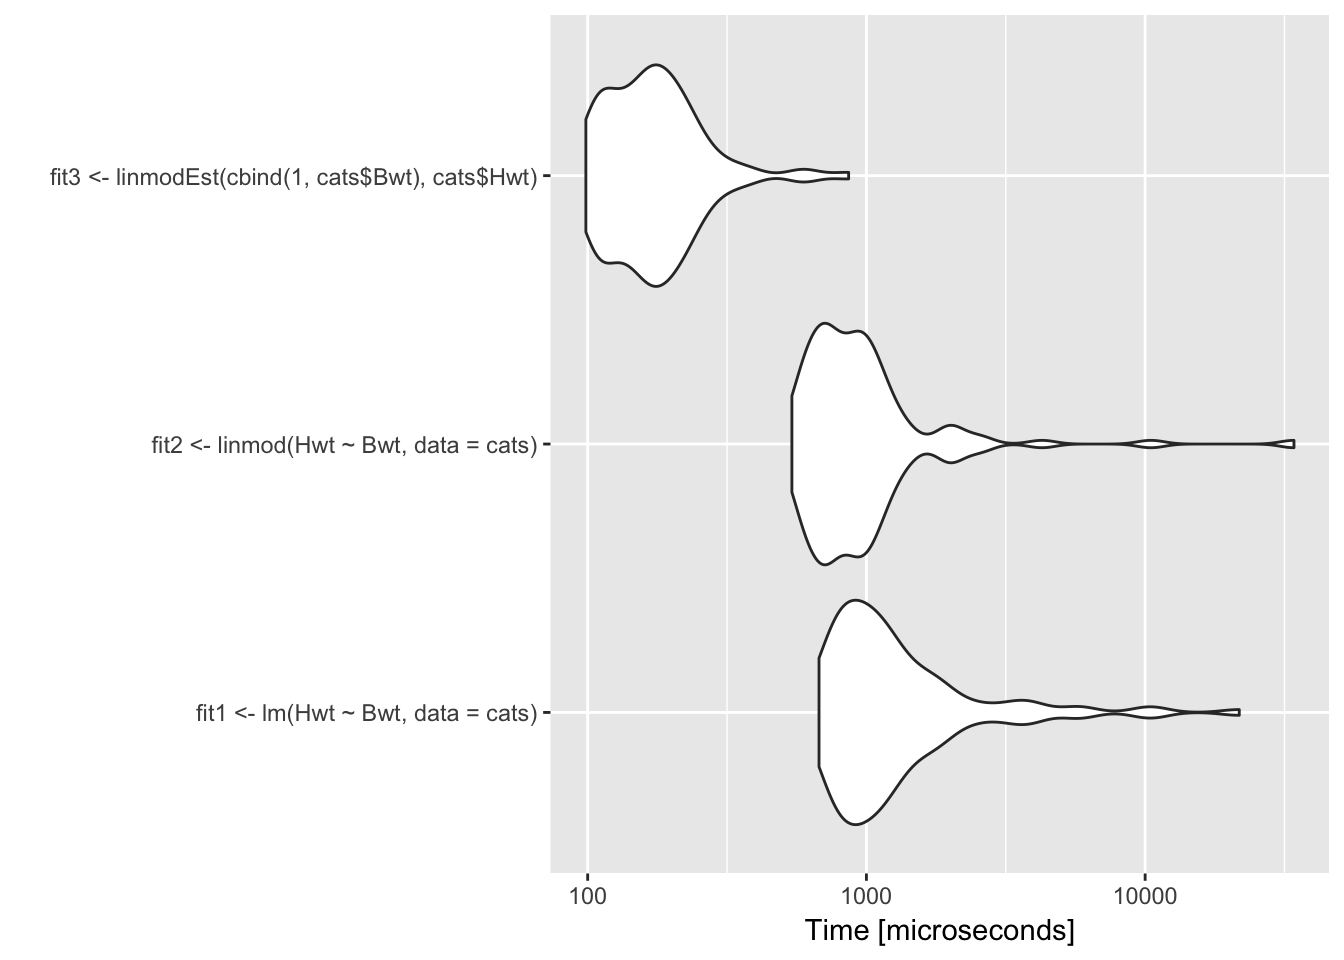
\includegraphics{Computing_for_Big_Data_files/figure-latex/unnamed-chunk-69-1.pdf}

\section{Improving performance}\label{improving-performance}

\begin{itemize}
\item
  Vectorize
\item
  Parallelize
\item
  Use a faster language (C/C++, Fortran, \ldots{})
\item
  Use different tools (as in Chapter \ref{bigdata})
\end{itemize}

\section{Vectorization}\label{vectorization}

Let's take an example from a blog post (that seems to be
\href{http://www.babelgraph.org/wp/?p=358}{gone}). It's used in
\citet[Section
\href{http://adv-r.had.co.nz/Rcpp.html\#rcpp-case-studies}{Case
studies}]{Wickham2014}.

\begin{Shaded}
\begin{Highlighting}[]
\NormalTok{vacc1a <-}\StringTok{ }\ControlFlowTok{function}\NormalTok{(age, female, ily) \{}
\NormalTok{  p <-}\StringTok{ }\FloatTok{0.25} \OperatorTok{+}\StringTok{ }\FloatTok{0.3} \OperatorTok{*}\StringTok{ }\DecValTok{1} \OperatorTok{/}\StringTok{ }\NormalTok{(}\DecValTok{1} \OperatorTok{-}\StringTok{ }\KeywordTok{exp}\NormalTok{(}\FloatTok{0.04} \OperatorTok{*}\StringTok{ }\NormalTok{age)) }\OperatorTok{+}\StringTok{ }\FloatTok{0.1} \OperatorTok{*}\StringTok{ }\NormalTok{ily}
\NormalTok{  p <-}\StringTok{ }\NormalTok{p }\OperatorTok{*}\StringTok{ }\ControlFlowTok{if}\NormalTok{ (female) }\FloatTok{1.25} \ControlFlowTok{else} \FloatTok{0.75}
\NormalTok{  p <-}\StringTok{ }\KeywordTok{max}\NormalTok{(}\DecValTok{0}\NormalTok{, p)}
\NormalTok{  p <-}\StringTok{ }\KeywordTok{min}\NormalTok{(}\DecValTok{1}\NormalTok{, p)}
\NormalTok{  p}
\NormalTok{\}}

\KeywordTok{set.seed}\NormalTok{(}\DecValTok{1959}\NormalTok{)}
\NormalTok{n <-}\StringTok{ }\DecValTok{1000}
\NormalTok{age <-}\StringTok{ }\KeywordTok{rnorm}\NormalTok{(n, }\DataTypeTok{mean =} \DecValTok{50}\NormalTok{, }\DataTypeTok{sd =} \DecValTok{10}\NormalTok{)}
\NormalTok{female <-}\StringTok{ }\KeywordTok{sample}\NormalTok{(}\KeywordTok{c}\NormalTok{(T, F), n, }\DataTypeTok{rep =} \OtherTok{TRUE}\NormalTok{)}
\NormalTok{ily <-}\StringTok{ }\KeywordTok{sample}\NormalTok{(}\KeywordTok{c}\NormalTok{(T, F), n, }\DataTypeTok{prob =} \KeywordTok{c}\NormalTok{(}\FloatTok{0.8}\NormalTok{, }\FloatTok{0.2}\NormalTok{), }\DataTypeTok{rep =} \OtherTok{TRUE}\NormalTok{)}

\KeywordTok{vacc1a}\NormalTok{(age[}\DecValTok{1}\NormalTok{], female[}\DecValTok{1}\NormalTok{], ily[}\DecValTok{1}\NormalTok{])}
\end{Highlighting}
\end{Shaded}

\begin{verbatim}
## [1] 0.1667005
\end{verbatim}

\begin{Shaded}
\begin{Highlighting}[]
\KeywordTok{vacc1a}\NormalTok{(age[}\DecValTok{2}\NormalTok{], female[}\DecValTok{2}\NormalTok{], ily[}\DecValTok{2}\NormalTok{])}
\end{Highlighting}
\end{Shaded}

\begin{verbatim}
## [1] 0.4045439
\end{verbatim}

\begin{Shaded}
\begin{Highlighting}[]
\KeywordTok{vacc1a}\NormalTok{(age[}\DecValTok{3}\NormalTok{], female[}\DecValTok{3}\NormalTok{], ily[}\DecValTok{3}\NormalTok{])}
\end{Highlighting}
\end{Shaded}

\begin{verbatim}
## [1] 0.2699324
\end{verbatim}

\texttt{vacc1a} is not designed for vector inputs

\begin{Shaded}
\begin{Highlighting}[]
\KeywordTok{vacc1a}\NormalTok{(age, female, ily)}
\end{Highlighting}
\end{Shaded}

\begin{verbatim}
## Warning in if (female) 1.25 else 0.75: the condition has length > 1 and
## only the first element will be used
\end{verbatim}

\begin{verbatim}
## [1] 0.2526293
\end{verbatim}

It should be called

\begin{Shaded}
\begin{Highlighting}[]
\KeywordTok{vacc1a}\NormalTok{(age[}\DecValTok{1}\NormalTok{], female[}\DecValTok{1}\NormalTok{], ily[}\DecValTok{1}\NormalTok{])}
\end{Highlighting}
\end{Shaded}

\begin{verbatim}
## [1] 0.1667005
\end{verbatim}

\begin{Shaded}
\begin{Highlighting}[]
\KeywordTok{vacc1a}\NormalTok{(age[}\DecValTok{2}\NormalTok{], female[}\DecValTok{2}\NormalTok{], ily[}\DecValTok{2}\NormalTok{])}
\end{Highlighting}
\end{Shaded}

\begin{verbatim}
## [1] 0.4045439
\end{verbatim}

\begin{Shaded}
\begin{Highlighting}[]
\KeywordTok{vacc1a}\NormalTok{(age[}\DecValTok{3}\NormalTok{], female[}\DecValTok{3}\NormalTok{], ily[}\DecValTok{3}\NormalTok{])}
\end{Highlighting}
\end{Shaded}

\begin{verbatim}
## [1] 0.2699324
\end{verbatim}

We can use a loop:

\begin{Shaded}
\begin{Highlighting}[]
\NormalTok{out <-}\StringTok{ }\KeywordTok{numeric}\NormalTok{(n)}
\ControlFlowTok{for}\NormalTok{ (i }\ControlFlowTok{in} \DecValTok{1}\OperatorTok{:}\NormalTok{n)}
\NormalTok{  out[i] <-}\StringTok{ }\KeywordTok{vacc1a}\NormalTok{(age[i], female[i], ily[i])}
\end{Highlighting}
\end{Shaded}

or one of the \texttt{apply} functions:

\begin{Shaded}
\begin{Highlighting}[]
\NormalTok{vacc0<-}\StringTok{ }\ControlFlowTok{function}\NormalTok{(age, female, ily) \{}
  \KeywordTok{sapply}\NormalTok{(}\DecValTok{1}\OperatorTok{:}\NormalTok{n, }\ControlFlowTok{function}\NormalTok{(i) }\KeywordTok{vacc1a}\NormalTok{(age[i], female[i], ily[i]))}
\NormalTok{\}}

\NormalTok{out0 <-}\StringTok{ }\KeywordTok{vacc0}\NormalTok{(age, female, ily)}
\end{Highlighting}
\end{Shaded}

\begin{Shaded}
\begin{Highlighting}[]
\KeywordTok{all.equal}\NormalTok{(out, out0)}
\end{Highlighting}
\end{Shaded}

\begin{verbatim}
## [1] TRUE
\end{verbatim}

But, it's convenient for the function to support vector inputs, instead
of relying on users writing their own wrappers. We can loop inside the
function body.

\begin{Shaded}
\begin{Highlighting}[]
\NormalTok{vacc1 <-}\StringTok{ }\ControlFlowTok{function}\NormalTok{(age, female, ily) \{}
\NormalTok{  n <-}\StringTok{ }\KeywordTok{length}\NormalTok{(age)}
\NormalTok{  out <-}\StringTok{ }\KeywordTok{numeric}\NormalTok{(n)}
  \ControlFlowTok{for}\NormalTok{ (i }\ControlFlowTok{in} \KeywordTok{seq_len}\NormalTok{(n)) \{}
\NormalTok{    out[i] <-}\StringTok{ }\KeywordTok{vacc1a}\NormalTok{(age[i], female[i], ily[i])}
\NormalTok{  \}}
\NormalTok{  out}
\NormalTok{\}}
\end{Highlighting}
\end{Shaded}

or we can rely on base R functions that accept vector inputs

\begin{Shaded}
\begin{Highlighting}[]
\NormalTok{vacc2 <-}\StringTok{ }\ControlFlowTok{function}\NormalTok{(age, female, ily) \{}
\NormalTok{  p <-}\StringTok{ }\FloatTok{0.25} \OperatorTok{+}\StringTok{ }\FloatTok{0.3} \OperatorTok{*}\StringTok{ }\DecValTok{1} \OperatorTok{/}\StringTok{ }\NormalTok{(}\DecValTok{1} \OperatorTok{-}\StringTok{ }\KeywordTok{exp}\NormalTok{(}\FloatTok{0.04} \OperatorTok{*}\StringTok{ }\NormalTok{age)) }\OperatorTok{+}\StringTok{ }\FloatTok{0.1} \OperatorTok{*}\StringTok{ }\NormalTok{ily}
\NormalTok{  p <-}\StringTok{ }\NormalTok{p }\OperatorTok{*}\StringTok{ }\KeywordTok{ifelse}\NormalTok{(female, }\FloatTok{1.25}\NormalTok{, }\FloatTok{0.75}\NormalTok{)}
\NormalTok{  p <-}\StringTok{ }\KeywordTok{pmax}\NormalTok{(}\DecValTok{0}\NormalTok{, p)}
\NormalTok{  p <-}\StringTok{ }\KeywordTok{pmin}\NormalTok{(}\DecValTok{1}\NormalTok{, p)}
\NormalTok{  p}
\NormalTok{\}}
\end{Highlighting}
\end{Shaded}

\section{Parallelization}\label{parallelization}

\begin{Shaded}
\begin{Highlighting}[]
\KeywordTok{library}\NormalTok{(parallel)}
\NormalTok{cores <-}\StringTok{ }\KeywordTok{detectCores}\NormalTok{()}
\NormalTok{cores}
\end{Highlighting}
\end{Shaded}

\begin{verbatim}
## [1] 4
\end{verbatim}

\begin{Shaded}
\begin{Highlighting}[]
\NormalTok{vacc3 <-}\StringTok{ }\ControlFlowTok{function}\NormalTok{(age, female, ily) \{}
  \KeywordTok{mcmapply}\NormalTok{(}\ControlFlowTok{function}\NormalTok{(i) }\KeywordTok{vacc1a}\NormalTok{(age[i], female[i], ily[i]), }\DecValTok{1}\OperatorTok{:}\NormalTok{n, }\DataTypeTok{mc.cores =}\NormalTok{ cores }\OperatorTok{-}\StringTok{ }\DecValTok{1}\NormalTok{)}
\NormalTok{\}}

\NormalTok{out3 <-}\StringTok{ }\KeywordTok{vacc3}\NormalTok{(age, female, ily)}
\end{Highlighting}
\end{Shaded}

\begin{Shaded}
\begin{Highlighting}[]
\KeywordTok{library}\NormalTok{(microbenchmark)}
\NormalTok{m <-}\StringTok{ }\KeywordTok{microbenchmark}\NormalTok{(}
  \DataTypeTok{vacc0 =} \KeywordTok{vacc0}\NormalTok{(age, female, ily),}
  \DataTypeTok{vacc1 =} \KeywordTok{vacc1}\NormalTok{(age, female, ily),}
  \DataTypeTok{vacc2 =} \KeywordTok{vacc2}\NormalTok{(age, female, ily),}
  \DataTypeTok{vacc3 =} \KeywordTok{vacc3}\NormalTok{(age, female, ily)}
\NormalTok{)}
\NormalTok{m}
\end{Highlighting}
\end{Shaded}

\begin{verbatim}
## Unit: microseconds
##   expr       min        lq       mean    median        uq       max neval
##  vacc0  2042.355  3349.736  4552.8067  3803.228  5320.949 19835.006   100
##  vacc1  2106.299  2475.339  3477.1346  2762.795  3389.323 13232.481   100
##  vacc2   112.700   160.636   546.3875   221.698   614.314  7536.343   100
##  vacc3 12891.545 19432.145 22898.9777 21261.046 23412.436 82110.084   100
\end{verbatim}

\begin{Shaded}
\begin{Highlighting}[]
\NormalTok{ggplot2}\OperatorTok{::}\KeywordTok{autoplot}\NormalTok{(m)}
\end{Highlighting}
\end{Shaded}

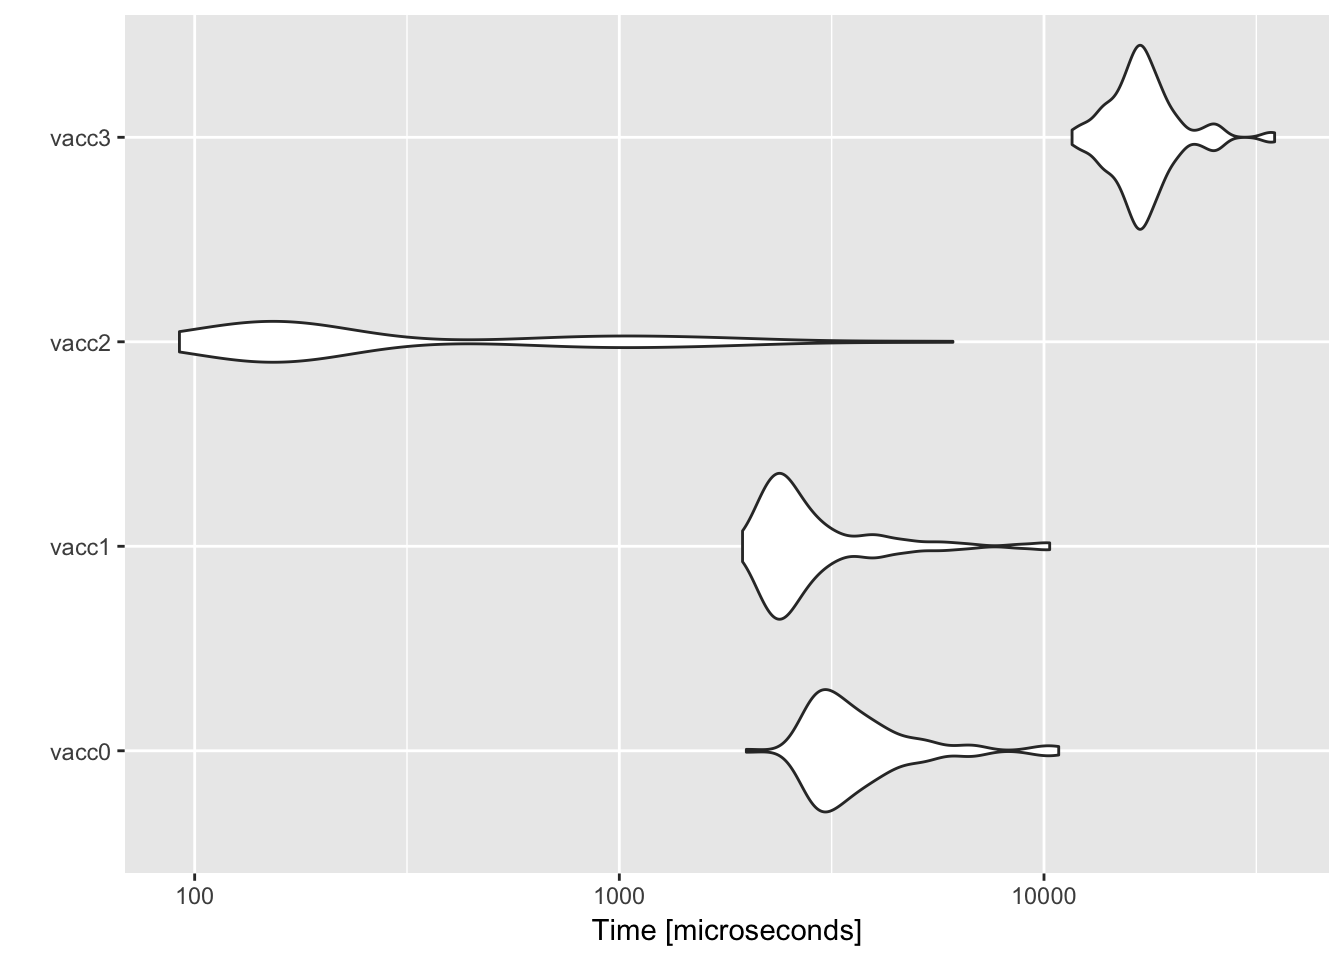
\includegraphics{Computing_for_Big_Data_files/figure-latex/unnamed-chunk-80-1.pdf}

So, what's going on?

We will talk more about parallelization tools and techniques in Chapter
`\citet{ref}(bigdata).

\section{Introduction to C++}\label{introduction-to-c}

\begin{itemize}
\item
  C++ is a very powerful object-oriented language.
\item
  Many tutorials are available on-line, for example
  \url{http://www.cplusplus.com/doc/tutorial/}.
\item
  R is \emph{intepreted}, C++ is \emph{compiled} and typically much
  faster (in loops for examples).
\item
  Our introduction to C++ is from an R perspective. Python (and most
  interpreted languages) can be extended with C++ too.
\end{itemize}

\subsection{Rcpp}\label{rcpp}

Reading: \url{http://adv-r.had.co.nz/Rcpp.html}

\begin{itemize}
\item
  \texttt{Rcpp} \citet{Eddelbuettel2013} makes it very easy to use C++
  code in R (for example to speed up a function or to wrap methods
  already implemented in C++).
\item
  \texttt{Rcpp} provides ``syntactic sugar'' that makes is easy to
  leverage C++ even without a deep knowledge of it.
\item
  To use \texttt{Rcpp}, you need a C++ compiler:

  \begin{itemize}
  \tightlist
  \item
    Windows:
    \href{https://cran.r-project.org/bin/windows/Rtools/}{Rtools}
  \item
    OS X: \href{https://developer.apple.com/xcode/}{Xcode}
  \item
    Linux: \texttt{r-base-dev} from package manager
  \end{itemize}
\end{itemize}

\subsection{Hello World!}\label{hello-world}

\begin{Shaded}
\begin{Highlighting}[]
\KeywordTok{library}\NormalTok{(Rcpp)}
\KeywordTok{cppFunction}\NormalTok{(}\StringTok{'void hello()\{}
\StringTok{  Rprintf("Hello, world!");}
\StringTok{\}'}\NormalTok{)}
\NormalTok{hello}
\end{Highlighting}
\end{Shaded}

\begin{verbatim}
## function () 
## invisible(.Primitive(".Call")(<pointer: 0x11081dcc0>))
\end{verbatim}

\begin{Shaded}
\begin{Highlighting}[]
\KeywordTok{hello}\NormalTok{()}
\end{Highlighting}
\end{Shaded}

\begin{verbatim}
## Hello, world!
\end{verbatim}

\texttt{Rprintf} is the counterpart of C++
\href{http://www.cplusplus.com/reference/cstdio/printf/}{\texttt{printf}}
function.

Let's take the first example of \citet{Wickham2014}, Section
\href{http://adv-r.had.co.nz/Rcpp.html\#rcpp-intro}{Getting started with
C++}.

\begin{Shaded}
\begin{Highlighting}[]
\KeywordTok{cppFunction}\NormalTok{(}\StringTok{'int add(int x, int y, int z) \{}
\StringTok{  int sum = x + y + z;}
\StringTok{  return sum;}
\StringTok{\}'}\NormalTok{)}
\end{Highlighting}
\end{Shaded}

We have to specify the input type and the output type. As expected

\begin{Shaded}
\begin{Highlighting}[]
\KeywordTok{add}\NormalTok{(}\DecValTok{1}\NormalTok{, }\DecValTok{2}\NormalTok{, }\DecValTok{3}\NormalTok{)}
\end{Highlighting}
\end{Shaded}

returns 6. How about?

\begin{Shaded}
\begin{Highlighting}[]
\KeywordTok{add}\NormalTok{(}\FloatTok{1.1}\NormalTok{, }\FloatTok{2.2}\NormalTok{, }\FloatTok{3.3}\NormalTok{)}
\end{Highlighting}
\end{Shaded}

\begin{Shaded}
\begin{Highlighting}[]
\KeywordTok{cppFunction}\NormalTok{(}\StringTok{'double addd(double x, double y, double z) \{}
\StringTok{  double sum = x + y + z;}
\StringTok{  return sum;}
\StringTok{\}'}\NormalTok{)}
\end{Highlighting}
\end{Shaded}

With \texttt{addd} we do get 6.6:

\begin{Shaded}
\begin{Highlighting}[]
\KeywordTok{addd}\NormalTok{(}\FloatTok{1.1}\NormalTok{, }\FloatTok{2.2}\NormalTok{, }\FloatTok{3.3}\NormalTok{)}
\end{Highlighting}
\end{Shaded}

\subsection{\texorpdfstring{\texttt{sourceCpp}}{sourceCpp}}\label{sourcecpp}

When C++ code takes more than a couple of lines, it's more convenient to
create a stand-alone C++ source file.

From the RStudio default template:

\begin{Shaded}
\begin{Highlighting}[]
\PreprocessorTok{#include }\ImportTok{<Rcpp.h>}
\KeywordTok{using} \KeywordTok{namespace}\NormalTok{ Rcpp;}

\NormalTok{NumericVector timesTwo(NumericVector x) \{}
  \ControlFlowTok{return}\NormalTok{ x * }\DecValTok{2}\NormalTok{;}
\NormalTok{\}}

\CommentTok{/*** R}
\CommentTok{timesTwo(42)}
\CommentTok{*/}
\end{Highlighting}
\end{Shaded}

From R, we can use \texttt{sourceCpp} to access \texttt{timesTwo} in R:

\begin{Shaded}
\begin{Highlighting}[]
\KeywordTok{sourceCpp}\NormalTok{(}\StringTok{"src/times-two.cpp"}\NormalTok{)}
\KeywordTok{timesTwo}\NormalTok{(}\DecValTok{100}\NormalTok{)}
\end{Highlighting}
\end{Shaded}

\subsection{Data types}\label{data-types}

\texttt{int} \texttt{double} \texttt{bool} \texttt{string}

\texttt{NumericVector} \texttt{LogicalVector} \texttt{IntegerVector}
\texttt{CharacterVector}

\texttt{NumericMatrix} \texttt{IntegerMatrix} \texttt{LogicalMatrix}
\texttt{CharacterMatrix}

\texttt{NA\_REAL} \texttt{NA\_INTEGER} \texttt{NA\_STRING}
\texttt{NA\_LOGICAL}

\texttt{List} \texttt{DataFrame} \texttt{Function}

\ldots{}

\subsection{Sugar}\label{sugar}

Reading: \url{http://adv-r.had.co.nz/Rcpp.html\#rcpp-sugar}.

\begin{itemize}
\item
  Vectorization of \texttt{+}, \texttt{*}, \texttt{-}, \texttt{/},
  \texttt{pow}, \texttt{\textless{}}, \texttt{\textless{}=},
  \texttt{\textgreater{}}, \texttt{\textgreater{}=}, \texttt{==},
  \texttt{!=}, \ldots{}
\item
  Vectorization of R-like functions: \texttt{abs()}, \texttt{exp()},
  \texttt{factorial()}, \ldots{}
\end{itemize}

\BeginKnitrBlock{exercise}
\protect\hypertarget{exr:unnamed-chunk-89}{}{\label{exr:unnamed-chunk-89}
}Can you write an \texttt{Rcpp} function similar to \texttt{addd} but
accepting vector arguments?
\EndKnitrBlock{exercise}

\begin{Shaded}
\begin{Highlighting}[]
\KeywordTok{cppFunction}\NormalTok{(}\StringTok{'NumericVector addv(NumericVector x, NumericVector y, NumericVector z) \{}
\StringTok{  NumericVector sum = x + y + z;}
\StringTok{  return sum;}
\StringTok{\}'}\NormalTok{)}
\end{Highlighting}
\end{Shaded}

\subsection{Example (continued)}\label{example-continued}

\begin{Shaded}
\begin{Highlighting}[]
\PreprocessorTok{#include }\ImportTok{<Rcpp.h>}
\KeywordTok{using} \KeywordTok{namespace}\NormalTok{ Rcpp;}

\DataTypeTok{double}\NormalTok{ vacc3a(}\DataTypeTok{double}\NormalTok{ age, }\DataTypeTok{bool}\NormalTok{ female, }\DataTypeTok{bool}\NormalTok{ ily)\{}
  \DataTypeTok{double}\NormalTok{ p = }\FloatTok{0.25}\NormalTok{ + }\FloatTok{0.3}\NormalTok{ * }\DecValTok{1}\NormalTok{ / (}\DecValTok{1}\NormalTok{ - exp(}\FloatTok{0.04}\NormalTok{ * age)) + }\FloatTok{0.1}\NormalTok{ * ily;}
\NormalTok{  p = p * (female ? }\FloatTok{1.25}\NormalTok{ : }\FloatTok{0.75}\NormalTok{);}
\NormalTok{  p = }\BuiltInTok{std::}\NormalTok{max(p, }\FloatTok{0.0}\NormalTok{);}
\NormalTok{  p = }\BuiltInTok{std::}\NormalTok{min(p, }\FloatTok{1.0}\NormalTok{);}
  \ControlFlowTok{return}\NormalTok{ p;}
\NormalTok{\}}

\CommentTok{// [[Rcpp::export]]}
\NormalTok{NumericVector vacc3(NumericVector age, LogicalVector female, }
\NormalTok{                    LogicalVector ily) \{}
  \DataTypeTok{int}\NormalTok{ n = age.size();}
\NormalTok{  NumericVector out(n);}

  \ControlFlowTok{for}\NormalTok{(}\DataTypeTok{int}\NormalTok{ i = }\DecValTok{0}\NormalTok{; i < n; ++i) \{}
\NormalTok{    out[i] = vacc3a(age[i], female[i], ily[i]);}
\NormalTok{  \}}

  \ControlFlowTok{return}\NormalTok{ out;}
\NormalTok{\}}
\end{Highlighting}
\end{Shaded}

\subsection{Back to Linreg}\label{back-to-linreg}

\begin{itemize}
\item
  \texttt{armadillo} is a very powerful C++ linear algebra library:
  \url{http://arma.sourceforge.net/}
\item
  It can be used in \texttt{Rcpp} via the \texttt{RcppArmadillo}
  package.
\end{itemize}

\BeginKnitrBlock{exercise}
\protect\hypertarget{exr:unnamed-chunk-92}{}{\label{exr:unnamed-chunk-92}
}Can you write an \texttt{Rcpp} function similar to \texttt{linmodEst}?
\EndKnitrBlock{exercise}

\begin{Shaded}
\begin{Highlighting}[]
\NormalTok{linmodEst <-}\StringTok{ }\ControlFlowTok{function}\NormalTok{(x, y) \{}
\NormalTok{  ## CC: crossprod or a QR decomposition (as in the original version) are more efficient}
\NormalTok{  coef <-}\StringTok{ }\KeywordTok{solve}\NormalTok{(}\KeywordTok{t}\NormalTok{(x) }\OperatorTok\StringTok{ }\NormalTok{x) }\OperatorTok\StringTok{ }\KeywordTok{t}\NormalTok{(x) }\OperatorTok\StringTok{ }\NormalTok{y}
\NormalTok{  ## degrees of freedom and standard deviation of residuals}
\NormalTok{  df <-}\StringTok{ }\KeywordTok{nrow}\NormalTok{(x) }\OperatorTok{-}\StringTok{ }\KeywordTok{ncol}\NormalTok{(x)}
\NormalTok{  sigma2 <-}\StringTok{ }\KeywordTok{sum}\NormalTok{((y }\OperatorTok{-}\StringTok{ }\NormalTok{x }\OperatorTok\StringTok{ }\NormalTok{coef) }\OperatorTok{^}\StringTok{ }\DecValTok{2}\NormalTok{) }\OperatorTok{/}\StringTok{ }\NormalTok{df}
\NormalTok{  ## compute sigma^2 * (x’x)^-1}
\NormalTok{  vcov <-}\StringTok{ }\NormalTok{sigma2 }\OperatorTok{*}\StringTok{ }\KeywordTok{solve}\NormalTok{(}\KeywordTok{t}\NormalTok{(x) }\OperatorTok\StringTok{ }\NormalTok{x)}
  \KeywordTok{colnames}\NormalTok{(vcov) <-}\StringTok{ }\KeywordTok{rownames}\NormalTok{(vcov) <-}\StringTok{ }\KeywordTok{colnames}\NormalTok{(x)}
  \KeywordTok{list}\NormalTok{(}
    \DataTypeTok{coefficients =}\NormalTok{ coef,}
    \DataTypeTok{vcov =}\NormalTok{ vcov,}
    \DataTypeTok{sigma =} \KeywordTok{sqrt}\NormalTok{(sigma2),}
    \DataTypeTok{df =}\NormalTok{ df}
\NormalTok{  )}
\NormalTok{\}}
\end{Highlighting}
\end{Shaded}

\section{Rcpp packages}\label{rcpp-packages}

Readings: -
\url{https://cran.r-project.org/web/packages/Rcpp/vignettes/Rcpp-package.pdf}
- \url{http://adv-r.had.co.nz/Rcpp.html\#rcpp-package}

\section{Getting serious about C++}\label{getting-serious-about-c}

\subsection{STL}\label{stl}

STL: Standard Template Library

Reading: \url{http://adv-r.had.co.nz/Rcpp.html\#stl}

\section{Profiling}\label{profiling}

Reading: \url{https://rstudio.github.io/profvis/}

\begin{Shaded}
\begin{Highlighting}[]
\KeywordTok{library}\NormalTok{(profvis)}

\KeywordTok{profvis}\NormalTok{(\{}
  \KeywordTok{data}\NormalTok{(diamonds, }\DataTypeTok{package =} \StringTok{"ggplot2"}\NormalTok{)}

  \KeywordTok{plot}\NormalTok{(price }\OperatorTok{~}\StringTok{ }\NormalTok{carat, }\DataTypeTok{data =}\NormalTok{ diamonds)}
\NormalTok{  m <-}\StringTok{ }\KeywordTok{lm}\NormalTok{(price }\OperatorTok{~}\StringTok{ }\NormalTok{carat, }\DataTypeTok{data =}\NormalTok{ diamonds)}
  \KeywordTok{abline}\NormalTok{(m, }\DataTypeTok{col =} \StringTok{"red"}\NormalTok{)}
\NormalTok{\})}
\end{Highlighting}
\end{Shaded}

\chapter{Databases}\label{databases}

\section{What is SQL?}\label{what-is-sql}

SQL (Structured Query Language) is a standard way of specifying the
information you want to receive from a database. There are a number of
variations on the language, and a number of online resources available
for learning their various complexities. However, the general structure
of all SQL queries is consistent across implementations.

SQL is an imperative computer language. This means that it describes the
output desired without actually describing the calculations required to
get the output described. This allows for the verbs and structures of
the language to be used across database systems, as well as in other
areas of data handling.

\subsection{What is a database?}\label{what-is-a-database}

A database is simply an organized structure for storing and accessing
data on disk. There are a number of structures used to store data on
disk, each with their own languages. However, despite the variations in
structure, the goals (and song) remain the same. The process of data
storage on disk is controlled by the database management system (DBMS).

\subsection{Relational Databases (SQL)}\label{relational-databases-sql}

The most common type of DBMS is a relational database (RDBMS). A
Relational Database stores information in a the form of entities and the
relationships between them. Entities are typically nouns and
relationships are typically verbs. For example, if we wanted to store
information about class enrollment at a university, the entities would
consist of objects like a student, class, and professor. The
relationships would consist of takes and teaches. Relationships can be
one to one, many to many, or one to many.

\subsection{Types of Relational
Databases}\label{types-of-relational-databases}

\begin{itemize}
\tightlist
\item
  Commercial

  \begin{itemize}
  \tightlist
  \item
    Oracle Database
  \item
    Microsoft
  \item
    SQL Server
  \item
    \ldots{}
  \end{itemize}
\item
  Open-source

  \begin{itemize}
  \tightlist
  \item
    MySQL
  \item
    PostgreSQL
  \item
    SQLite
  \item
    \ldots{}
  \end{itemize}
\item
  SQLite is the easiest way to start: unlike the others, it's not a
  client-server DB. The whole DB can live in a (portable) folder. All
  the required tools are included in \texttt{dplyr}.
\end{itemize}

\subsection{SQL}\label{sql}

In relational databases, entities and relationships are represented by
tables, where each row or record in a table represents a particular
instance of of that general object. Continuing the class example,
students would be stored in \texttt{Student}, classes in \texttt{Class},
and professors in \texttt{Professor}. The table containing the
relationships between students and classes would be likely named
\texttt{StudentClass} and the

The three key parts of a SQL query are the \texttt{SELECT} clause, the
\texttt{FROM} clause, and the \texttt{WHERE} clause. The \texttt{SELECT}
clause specifies the pieces of information you want about an individual
record, the \texttt{FROM} clause specifies the tables that will be used

To get all information about all students we would type the following:

\begin{Shaded}
\begin{Highlighting}[]
\KeywordTok{SELECT}\NormalTok{ * }\KeywordTok{FROM}\NormalTok{ STUDENT}
\end{Highlighting}
\end{Shaded}

To Select the name and birthday of all students in classes taught by
Dr.~Choirat would be a more complex query, which would likely look
something like this:

\begin{Shaded}
\begin{Highlighting}[]
   \KeywordTok{SELECT}\NormalTok{ Name,}
\NormalTok{          DOB}
   \KeywordTok{FROM}\NormalTok{ Student s }
        \KeywordTok{inner} \KeywordTok{join}\NormalTok{ StudentClass sc }\KeywordTok{on} 
\NormalTok{            s.ID = sc.studentid}
        \KeywordTok{inner} \KeywordTok{join}\NormalTok{ ProfessorClass pc }\KeywordTok{on}
\NormalTok{            sc.classid = pc.classid}
        \KeywordTok{inner} \KeywordTok{join}\NormalTok{ Professor p }\KeywordTok{on}
\NormalTok{            pc.profid = p.id}
    \KeywordTok{WHERE}\NormalTok{ p.lastname = }\OtherTok{"Choirat"}
\end{Highlighting}
\end{Shaded}

\section{SQLite: An Exercise}\label{sqlite-an-exercise}

Create an in memory DB

\texttt{sqlite3}

\subsection{Make a Table}\label{make-a-table}

\begin{Shaded}
\begin{Highlighting}[]
\KeywordTok{CREATE} \KeywordTok{TABLE}\NormalTok{ table1(x,y,z);}
\end{Highlighting}
\end{Shaded}

\subsection{Insert Values}\label{insert-values}

\begin{Shaded}
\begin{Highlighting}[]
\KeywordTok{INSERT} \KeywordTok{INTO}\NormalTok{ table1 }\KeywordTok{VALUES}\NormalTok{ (}\DecValTok{1}\NormalTok{,}\DecValTok{2}\NormalTok{,}\DecValTok{3}\NormalTok{),(}\DecValTok{4}\NormalTok{,}\DecValTok{5}\NormalTok{,}\DecValTok{6}\NormalTok{),(}\DecValTok{7}\NormalTok{,}\DecValTok{8}\NormalTok{,}\DecValTok{9}\NormalTok{);}
\end{Highlighting}
\end{Shaded}

\subsection{Select Values}\label{select-values}

Select All Values

\begin{Shaded}
\begin{Highlighting}[]
\KeywordTok{SELECT}\NormalTok{ * }\KeywordTok{FROM}\NormalTok{ table1;}
\end{Highlighting}
\end{Shaded}

Select specific values

\begin{Shaded}
\begin{Highlighting}[]
\KeywordTok{SELECT}\NormalTok{ z }\KeywordTok{from}\NormalTok{ table1 }\KeywordTok{WHERE}\NormalTok{ x = }\DecValTok{4}\NormalTok{;}
\end{Highlighting}
\end{Shaded}

\section{SQL and R}\label{sql-and-r}

There are a number of R packages for interfacing directly with RDBs.
RODBC is one sucn example that allows for queries to be submitted to
previsously set up database connections with the results being returned
as a data frame for further analysis in R. There's a large amount of
documentation available online for these methods. Each system has its
own idiosyncracies.

\subsection{\texorpdfstring{Data: \texttt{oscars} and \texttt{movies}
again: 2016 Oscars
Nominations}{Data: oscars and movies again: 2016 Oscars Nominations}}\label{data-oscars-and-movies-again-2016-oscars-nominations}

\begin{Shaded}
\begin{Highlighting}[]
\KeywordTok{library}\NormalTok{(readr)}
\KeywordTok{library}\NormalTok{(dplyr)}

\NormalTok{db <-}\StringTok{ }\KeywordTok{src_sqlite}\NormalTok{(}\StringTok{"db.sqlite3"}\NormalTok{, }\DataTypeTok{create =} \OtherTok{TRUE}\NormalTok{)}

\NormalTok{oscars <-}\StringTok{"}
\StringTok{name,movie,category}
\StringTok{Adam McKay,The Big Short,Best Director}
\StringTok{Alejandro González Iñárritu,The Revenant,Best Director}
\StringTok{Lenny Abrahamson,Room,Best Director}
\StringTok{Tom McCarthy,Spotlight,Best Director}
\StringTok{George Miller,Mad Max: Fury Road,Best Director}
\StringTok{Bryan Cranston,Trumbo,Best Actor}
\StringTok{Matt Damon,The Martian,Best Actor}
\StringTok{Michael Fassbender,Steve Jobs,Best Actor}
\StringTok{Leonardo DiCaprio,The Revenant,Best Actor}
\StringTok{Eddie Redmayne,The Danish Girl,Best Actor}
\StringTok{Cate Blanchett,Carol,Best Actress}
\StringTok{Brie Larson,Room,Best Actress}
\StringTok{Jennifer Lawrence,Joy,Best Actress}
\StringTok{Charlotte Rampling,45 Years,Best Actress}
\StringTok{Saoirse Ronan,Brooklyn,Best Actress}
\StringTok{"}
\NormalTok{oscars <-}\StringTok{ }\KeywordTok{read_csv}\NormalTok{(oscars, }\DataTypeTok{trim_ws =} \OtherTok{TRUE}\NormalTok{, }\DataTypeTok{skip =} \DecValTok{1}\NormalTok{)}

\NormalTok{movies <-}\StringTok{"}
\StringTok{movie,length_mins}
\StringTok{The Big Short,130}
\StringTok{Star Wars: The Force Awakens,135}
\StringTok{Brooklyn,111}
\StringTok{Mad Max: Fury Road,120}
\StringTok{Room,118}
\StringTok{The Martian,144}
\StringTok{The Revenant,156}
\StringTok{Spotlight,128}
\StringTok{"}
\NormalTok{movies <-}\StringTok{ }\KeywordTok{read_csv}\NormalTok{(movies, }\DataTypeTok{trim_ws =} \OtherTok{TRUE}\NormalTok{, }\DataTypeTok{skip =} \DecValTok{1}\NormalTok{)}

\NormalTok{oscars_table <-}\StringTok{ }\KeywordTok{copy_to}\NormalTok{(db, oscars)}
\NormalTok{movies_table <-}\StringTok{ }\KeywordTok{copy_to}\NormalTok{(db, movies)}

\NormalTok{db}
\end{Highlighting}
\end{Shaded}

\section{Non-Relational Databases
(noSQL)}\label{non-relational-databases-nosql}

\subsection{Drawbacks of Relational
Databases}\label{drawbacks-of-relational-databases}

\begin{itemize}
\tightlist
\item
  Looking up all information about one entity can be expensive
\item
  Require a large amount of overhead
\item
  Difficult to distribute across multiple disks
\item
  Considered to by some to be inflexible
\end{itemize}

\subsection{Common Types of NoSQL
Databases}\label{common-types-of-nosql-databases}

\begin{itemize}
\tightlist
\item
  Graph Databases

  \begin{itemize}
  \tightlist
  \item
    Neo4j
  \item
    OrientDB
  \end{itemize}
\item
  Document Databases

  \begin{itemize}
  \tightlist
  \item
    MongoDB
  \item
    JSON Databases
  \item
    XML Databases
  \end{itemize}
\end{itemize}

\section{References}\label{references}

The Oscar movie example comes from this lecture by Rafa Irizarry:
\url{https://github.com/datasciencelabs/2016/blob/master/lectures/wrangling/data-wrangling-with-dplyr.Rmd}

\section{NoSQL: MongoDB}\label{nosql-mongodb}

\subsection{JSON format}\label{json-format}

JSON: \textbf{J}ava\textbf{S}cript \textbf{O}bject \textbf{N}otation.

Readings:

\begin{itemize}
\tightlist
\item
  \url{http://www.json.org/}
\item
  \url{http://json.org/example.html}
\item
  \url{https://cran.r-project.org/web/packages/jsonlite/vignettes/json-aaquickstart.html}
\end{itemize}

\begin{Shaded}
\begin{Highlighting}[]
\KeywordTok{library}\NormalTok{(jsonlite)}
\NormalTok{l <-}\StringTok{ }\KeywordTok{fromJSON}\NormalTok{(}
  \StringTok{'\{}
\StringTok{    "glossary": \{}
\StringTok{        "title": "example glossary",}
\StringTok{        "GlossDiv": \{}
\StringTok{            "title": "S",}
\StringTok{            "GlossList": \{}
\StringTok{                "GlossEntry": \{}
\StringTok{                    "ID": "SGML",}
\StringTok{                    "SortAs": "SGML",}
\StringTok{                    "GlossTerm": "Standard Generalized Markup Language",}
\StringTok{                    "Acronym": "SGML",}
\StringTok{                    "Abbrev": "ISO 8879:1986",}
\StringTok{                    "GlossDef": \{}
\StringTok{                        "para": "A meta-markup language, used to create markup languages such as DocBook.",}
\StringTok{                        "GlossSeeAlso": ["GML", "XML"]}
\StringTok{                    \},}
\StringTok{                    "GlossSee": "markup"}
\StringTok{                \}}
\StringTok{            \}}
\StringTok{        \}}
\StringTok{    \}}
\StringTok{\}'}
\NormalTok{)}
\NormalTok{l}\OperatorTok{$}\NormalTok{glossary}\OperatorTok{$}\NormalTok{title}
\end{Highlighting}
\end{Shaded}

\begin{verbatim}
## [1] "example glossary"
\end{verbatim}

\begin{Shaded}
\begin{Highlighting}[]
\NormalTok{l}\OperatorTok{$}\NormalTok{glossary}\OperatorTok{$}\NormalTok{GlossDiv}\OperatorTok{$}\NormalTok{GlossList}\OperatorTok{$}\NormalTok{GlossEntry}\OperatorTok{$}\NormalTok{GlossDef}
\end{Highlighting}
\end{Shaded}

\begin{verbatim}
## $para
## [1] "A meta-markup language, used to create markup languages such as DocBook."
## 
## $GlossSeeAlso
## [1] "GML" "XML"
\end{verbatim}

\begin{Shaded}
\begin{Highlighting}[]
\NormalTok{l <-}\StringTok{ }\KeywordTok{fromJSON}\NormalTok{(}\StringTok{"src/example.json"}\NormalTok{)}
\end{Highlighting}
\end{Shaded}

\subsection{Reading a JSON file}\label{reading-a-json-file}

\begin{Shaded}
\begin{Highlighting}[]
\NormalTok{l <-}\StringTok{ }\KeywordTok{fromJSON}\NormalTok{(}\StringTok{"~/Dropbox/Data17/citibike/stations_2017-11-25.json"")}
\end{Highlighting}
\end{Shaded}

\subsection{RESTful APIs}\label{restful-apis}

REST: \textbf{Re}presentational \textbf{S}tate \textbf{T}ransfer

Readings:

\begin{itemize}
\tightlist
\item
  \url{https://spring.io/understanding/REST}
\item
  \url{https://en.wikipedia.org/wiki/Representational_state_transfer\#Applied_to_Web_services}
\item
  \url{https://cran.r-project.org/web/packages/jsonlite/vignettes/json-apis.html}
\end{itemize}

\subsection{Back and forth}\label{back-and-forth}

\begin{Shaded}
\begin{Highlighting}[]
\NormalTok{l <-}\StringTok{ }\KeywordTok{list}\NormalTok{(}
  \DataTypeTok{a =} \KeywordTok{data.frame}\NormalTok{(}\DataTypeTok{v1 =} \DecValTok{1}\OperatorTok{:}\DecValTok{5}\NormalTok{, }\DataTypeTok{v2 =}\NormalTok{ letters[}\DecValTok{1}\OperatorTok{:}\DecValTok{5}\NormalTok{]),}
  \DataTypeTok{b =} \KeywordTok{list}\NormalTok{(}\DataTypeTok{el1 =} \DecValTok{4}\NormalTok{, }\DataTypeTok{el2 =} \StringTok{"hello"}\NormalTok{)}
\NormalTok{)}
\NormalTok{l}
\end{Highlighting}
\end{Shaded}

\begin{verbatim}
## $a
##   v1 v2
## 1  1  a
## 2  2  b
## 3  3  c
## 4  4  d
## 5  5  e
## 
## $b
## $b$el1
## [1] 4
## 
## $b$el2
## [1] "hello"
\end{verbatim}

\begin{Shaded}
\begin{Highlighting}[]
\KeywordTok{toJSON}\NormalTok{(l)}
\end{Highlighting}
\end{Shaded}

\begin{verbatim}
## {"a":[{"v1":1,"v2":"a"},{"v1":2,"v2":"b"},{"v1":3,"v2":"c"},{"v1":4,"v2":"d"},{"v1":5,"v2":"e"}],"b":{"el1":[4],"el2":["hello"]}}
\end{verbatim}

\begin{Shaded}
\begin{Highlighting}[]
\KeywordTok{toJSON}\NormalTok{(l, }\DataTypeTok{pretty =} \OtherTok{TRUE}\NormalTok{)}
\end{Highlighting}
\end{Shaded}

\begin{verbatim}
## {
##   "a": [
##     {
##       "v1": 1,
##       "v2": "a"
##     },
##     {
##       "v1": 2,
##       "v2": "b"
##     },
##     {
##       "v1": 3,
##       "v2": "c"
##     },
##     {
##       "v1": 4,
##       "v2": "d"
##     },
##     {
##       "v1": 5,
##       "v2": "e"
##     }
##   ],
##   "b": {
##     "el1": [4],
##     "el2": ["hello"]
##   }
## }
\end{verbatim}

\begin{Shaded}
\begin{Highlighting}[]
\NormalTok{ll <-}\StringTok{ }\KeywordTok{fromJSON}\NormalTok{(}\KeywordTok{toJSON}\NormalTok{(l))}
\end{Highlighting}
\end{Shaded}

\subsection{MongoDB}\label{mongodb}

Reading:
\url{https://docs.mongodb.com/manual/administration/install-community/}

With \texttt{homebrew} on OS X:

\begin{Shaded}
\begin{Highlighting}[]
\ExtensionTok{brew}\NormalTok{ update}
\ExtensionTok{brew}\NormalTok{ install mongodb}
\ExtensionTok{brew}\NormalTok{ tap homebrew/services }\CommentTok{# once}
\ExtensionTok{brew}\NormalTok{ services start mongodb}
\end{Highlighting}
\end{Shaded}

\subsection{Querying data}\label{querying-data}

Reading: \url{https://jeroen.github.io/mongolite/query-data.html}

\subsection{Example: mHealth data}\label{example-mhealth-data}

\begin{Shaded}
\begin{Highlighting}[]
\KeywordTok{system}\NormalTok{(}\StringTok{"mongoimport --db mhealth --collection sleep --drop --file ~/Dropbox/Data17/mHealth/sleep-duration.json"}\NormalTok{)}
\end{Highlighting}
\end{Shaded}

\begin{Shaded}
\begin{Highlighting}[]
\KeywordTok{library}\NormalTok{(mongolite)}
\NormalTok{mhealth <-}\StringTok{ }\KeywordTok{mongo}\NormalTok{(}\DataTypeTok{db =} \StringTok{"mhealth"}\NormalTok{)}
\NormalTok{sleep <-}\StringTok{ }\KeywordTok{mongo}\NormalTok{(}\DataTypeTok{collection =} \StringTok{"sleep"}\NormalTok{, }\DataTypeTok{db =} \StringTok{"mhealth"}\NormalTok{)}
\NormalTok{sleep}\OperatorTok{$}\KeywordTok{count}\NormalTok{(}\StringTok{'\{\}'}\NormalTok{) }\CommentTok{# 52 records}
\NormalTok{alldata <-}\StringTok{ }\NormalTok{sleep}\OperatorTok{$}\KeywordTok{find}\NormalTok{(}\StringTok{'\{\}'}\NormalTok{)}
\NormalTok{alldata}
\NormalTok{sleep}\OperatorTok{$}\KeywordTok{find}\NormalTok{()}
\end{Highlighting}
\end{Shaded}

\chapter{Big data}\label{bigdata}

\section{How to deal with (very / too) large
datasets?}\label{how-to-deal-with-very-too-large-datasets}

\begin{enumerate}
\def\labelenumi{\arabic{enumi}.}
\tightlist
\item
  Use more RAM / processors / drive space\ldots{}
\item
  Use less data: (re)sample, \ldots{}
\item
  Use a database
\item
  Use specific R packages (\texttt{ff}, \texttt{bigmemory})
\item
  Use other tools
\end{enumerate}

\section{How big is big?}\label{how-big-is-big}

\begin{enumerate}
\def\labelenumi{\arabic{enumi}.}
\tightlist
\item
  Fits in RAM and on drive (but slow)
\item
  Doesn't fit in RAM but fits on drive
\item
  Doesn't fit in RAM and doesn't fit on drive
\end{enumerate}

\section{List of tools}\label{list-of-tools}

Reading: \citet{Varian2014}
(\href{http://pubs.aeaweb.org/doi/pdfplus/10.1257/jep.28.2.3}{PDF
available})

\begin{figure}

{\centering 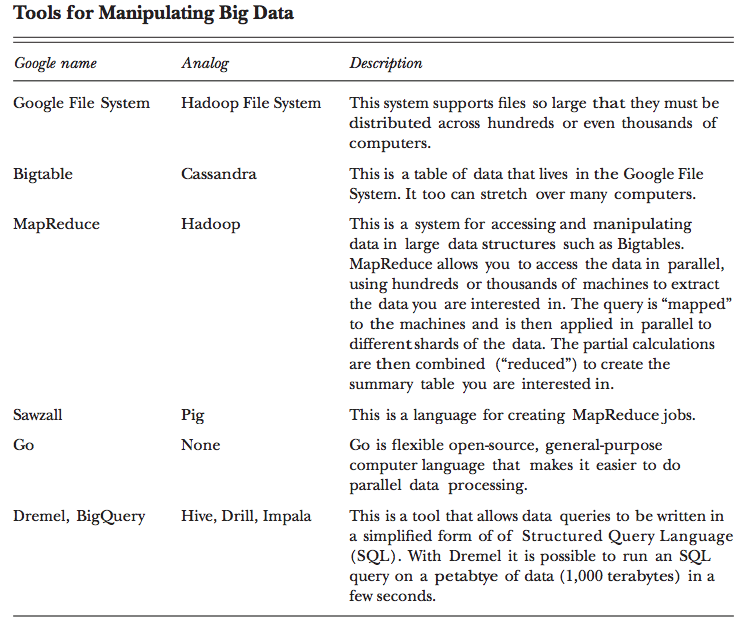
\includegraphics[width=10.39in]{images/ch6_tool_list} 

}

\end{figure}

Spark? h2o? More? Let's go back to the bottlenecks

\begin{itemize}
\tightlist
\item
  CPU
\item
  RAM
\item
  I/O
\end{itemize}

\section{Data that fits in memory}\label{data-that-fits-in-memory}

\subsection{Faster I/O}\label{faster-io}

Reading:
\url{https://cran.r-project.org/web/packages/data.table/vignettes/datatable-intro.html}

\texttt{data.table} provides an enhanced of a \texttt{data.frame} and
faster I/O with \texttt{fread} and \texttt{fwrite}.

To read the 0.5GB ratings file from MovieLens

\begin{Shaded}
\begin{Highlighting}[]
\KeywordTok{library}\NormalTok{(data.table)}
\KeywordTok{system.time}\NormalTok{(ratings <-}\StringTok{ }\KeywordTok{fread}\NormalTok{(}\StringTok{"~/Dropbox/Data17/ml-20m/ratings.csv"}\NormalTok{))}
\end{Highlighting}
\end{Shaded}

takes

\begin{verbatim}
Read 20000263 rows and 4 (of 4) columns from 0.497 GB file in 00:00:05
   user  system elapsed 
  4.007   0.229   4.244
\end{verbatim}

while

\begin{Shaded}
\begin{Highlighting}[]
\KeywordTok{system.time}\NormalTok{(ratings <-}\StringTok{ }\KeywordTok{read.csv}\NormalTok{(}\StringTok{"~/Dropbox/Data17/ml-20m/ratings.csv"}\NormalTok{))}
\end{Highlighting}
\end{Shaded}

takes

\begin{verbatim}
   user  system elapsed 
 85.199   2.711  90.997 
\end{verbatim}

There are ways to improve the speed of \texttt{read.csv} (for example,
but specifying column types). But in general \texttt{fread} is much
faster.

\begin{Shaded}
\begin{Highlighting}[]
\KeywordTok{library}\NormalTok{(readr) }\CommentTok{# in tidyverse}
\KeywordTok{system.time}\NormalTok{(ratings <-}\StringTok{ }\KeywordTok{read_csv}\NormalTok{(}\StringTok{"~/Dropbox/Data17/ml-20m/ratings.csv"}\NormalTok{))}
\end{Highlighting}
\end{Shaded}

\begin{verbatim}
   user  system elapsed 
 10.290   3.037  18.450 
\end{verbatim}

also tends to perform better than \texttt{read.csv}.

\begin{table}

\caption{\label{tab:unnamed-chunk-115}I/O comparison}
\centering
\begin{tabular}[t]{l|l|l|l}
\hline
package & function. & speed & output\\
\hline
base & read.csv & slow & data.frame\\
\hline
data.table & fread & very fast & data.table\\
\hline
readr & read\_csv & fast & tibble\\
\hline
\end{tabular}
\end{table}

\subsection{Reference vs copy}\label{reference-vs-copy}

Reading: \url{http://adv-r.had.co.nz/memory.html} Reading:
\url{https://jangorecki.gitlab.io/data.table/library/data.table/html/assign.html}

\begin{Shaded}
\begin{Highlighting}[]
\KeywordTok{library}\NormalTok{(pryr)}
\KeywordTok{library}\NormalTok{(data.table)}

\NormalTok{d <-}\StringTok{ }\KeywordTok{read.csv}\NormalTok{(}\StringTok{"~/Dropbox/Data17/ml-latest-small/ratings.csv"}\NormalTok{)}
\NormalTok{D <-}\StringTok{ }\KeywordTok{fread}\NormalTok{(}\StringTok{"~/Dropbox/Data17/ml-latest-small/ratings.csv"}\NormalTok{)}

\KeywordTok{object_size}\NormalTok{(d)}
\KeywordTok{object_size}\NormalTok{(D)}

\KeywordTok{mem_change}\NormalTok{(d}\OperatorTok{$}\NormalTok{Idx <-}\StringTok{ }\DecValTok{1}\OperatorTok{:}\KeywordTok{nrow}\NormalTok{(d))}
\KeywordTok{mem_change}\NormalTok{(D[, Idx}\OperatorTok{:}\ErrorTok{=}\StringTok{ }\DecValTok{1}\OperatorTok{:}\NormalTok{.N])}

\KeywordTok{object_size}\NormalTok{(d}\OperatorTok{$}\NormalTok{Idx)}
\KeywordTok{object_size}\NormalTok{(D}\OperatorTok{$}\NormalTok{Idx)}
\end{Highlighting}
\end{Shaded}

\begin{Shaded}
\begin{Highlighting}[]
\NormalTok{d <-}\StringTok{ }\KeywordTok{read.csv}\NormalTok{(}\StringTok{"~/Dropbox/Data17/ml-latest-small/ratings.csv"}\NormalTok{)}
\NormalTok{D <-}\StringTok{ }\KeywordTok{fread}\NormalTok{(}\StringTok{"~/Dropbox/Data17/ml-latest-small/ratings.csv"}\NormalTok{)}

\KeywordTok{.Internal}\NormalTok{(}\KeywordTok{inspect}\NormalTok{(d))}
\NormalTok{d}\OperatorTok{$}\NormalTok{Idx <-}\StringTok{ }\DecValTok{1}\OperatorTok{:}\KeywordTok{nrow}\NormalTok{(d)}
\KeywordTok{.Internal}\NormalTok{(}\KeywordTok{inspect}\NormalTok{(d))}

\KeywordTok{.Internal}\NormalTok{(}\KeywordTok{inspect}\NormalTok{(D))}
\NormalTok{D[, Idx}\OperatorTok{:}\ErrorTok{=}\StringTok{ }\DecValTok{1}\OperatorTok{:}\NormalTok{.N]}
\KeywordTok{.Internal}\NormalTok{(}\KeywordTok{inspect}\NormalTok{(D))}
\end{Highlighting}
\end{Shaded}

\subsection{data.table: another data manipulation
grammar}\label{data.table-another-data-manipulation-grammar}

Reading:
\url{https://cran.r-project.org/web/packages/data.table/vignettes/datatable-intro.html}

\BeginKnitrBlock{exercise}
\protect\hypertarget{exr:unnamed-chunk-118}{}{\label{exr:unnamed-chunk-118}
}Benchmark adding a column to a large data frame vs a large data table.
\EndKnitrBlock{exercise}

\section{Data that doesn't fit in memory (but fits on
drive)}\label{data-that-doesnt-fit-in-memory-but-fits-on-drive}

Let's try to work with a 12GB file and 4/8 GB of memory\ldots{}

\section{Pure R solutions}\label{pure-r-solutions}

\subsection{A regressions example}\label{a-regressions-example}

\begin{Shaded}
\begin{Highlighting}[]
\KeywordTok{library}\NormalTok{(data.table)}
\NormalTok{airlines <-}\StringTok{ }\KeywordTok{fread}\NormalTok{(}\StringTok{"/Users/cchoirat/Dropbox/Data17/AirFlights/allyears2k.csv"}\NormalTok{)}
\NormalTok{rfit <-}\StringTok{ }\KeywordTok{lm}\NormalTok{(ArrDelay }\OperatorTok{~}\StringTok{ }\NormalTok{Distance, }\DataTypeTok{data =}\NormalTok{ airlines)}
\KeywordTok{summary}\NormalTok{(rfit)}
\end{Highlighting}
\end{Shaded}

\subsection{Sampling}\label{sampling}

\begin{itemize}
\tightlist
\item
  Read the data (even line by line)
\item
  Select a sample of rows
\item
  Run your model on the random sample
\end{itemize}

\subsection{\texorpdfstring{\texttt{bigmemory}}{bigmemory}}\label{bigmemory}

\url{https://cran.r-project.org/web/packages/bigmemory/index.html}

Reading:
\url{https://cran.r-project.org/web/packages/bigmemory/vignettes/Overview.pdf}

\textbf{bigmemory}: Manage Massive Matrices with Shared Memory and
Memory-Mapped Files

Create, store, access, and manipulate massive matrices. Matrices are
allocated to shared memory and may use memory-mapped files. Packages
`biganalytics', `bigtabulate', `synchronicity', and `bigalgebra' provide
advanced functionality.

\textbf{(+)} pure R solution from a user perspective

\textbf{(-)} mostly for numeric data matrices, mostly to speed up
computations on data of +/- RAM size

\begin{Shaded}
\begin{Highlighting}[]
\KeywordTok{library}\NormalTok{(bigmemory)}
\KeywordTok{library}\NormalTok{(biganalytics)}
\CommentTok{# library(bigtabulate)}
\CommentTok{# library(biglm)}

\NormalTok{flights <-}\StringTok{ }\KeywordTok{read.big.matrix}\NormalTok{(}
  \StringTok{"/Users/cchoirat/Dropbox/Data17/AirFlights/allyears2k.csv"}\NormalTok{,}
  \DataTypeTok{header =} \OtherTok{TRUE}\NormalTok{,}
  \DataTypeTok{backingfile =} \StringTok{"allyears2k.bin"}\NormalTok{,}
  \DataTypeTok{backingpath =} \StringTok{"/Users/cchoirat/Dropbox/Data17/AirFlights/"}\NormalTok{,}
  \DataTypeTok{descriptorfile =} \StringTok{"allyears2k.desc"}\NormalTok{,}
  \DataTypeTok{shared =} \OtherTok{TRUE}\NormalTok{)}

\NormalTok{air_flights <-}\StringTok{ }\KeywordTok{attach.big.matrix}\NormalTok{(}\StringTok{"/Users/cchoirat/Dropbox/Data17/AirFlights/allyears2k.desc"}\NormalTok{)}
\KeywordTok{dim}\NormalTok{(air_flights)}
\KeywordTok{colnames}\NormalTok{(air_flights)}
\KeywordTok{mean}\NormalTok{(air_flights[, }\StringTok{"ArrDelay"}\NormalTok{], }\DataTypeTok{na.rm =} \OtherTok{TRUE}\NormalTok{)}

\NormalTok{fit <-}\StringTok{ }\KeywordTok{biglm.big.matrix}\NormalTok{(ArrDelay }\OperatorTok{~}\StringTok{ }\NormalTok{Distance, }\DataTypeTok{data =}\NormalTok{ air_flights)}
\NormalTok{fit}
\KeywordTok{summary}\NormalTok{(fit)}
\end{Highlighting}
\end{Shaded}

\subsection{Database connections and lazy
evaluation}\label{database-connections-and-lazy-evaluation}

\begin{Shaded}
\begin{Highlighting}[]
\KeywordTok{library}\NormalTok{(data.table)}
\NormalTok{D <-}\StringTok{ }\KeywordTok{fread}\NormalTok{(}\StringTok{"~/Dropbox/Data17/ml-20m/ratings.csv"}\NormalTok{)}

\KeywordTok{library}\NormalTok{(sqldf)}
\KeywordTok{read.csv.sql}\NormalTok{(}\DataTypeTok{file =} \StringTok{"~/Dropbox/Data17/ml-20m/ratings.csv"}\NormalTok{,}
             \DataTypeTok{sql =} \KeywordTok{c}\NormalTok{(}\StringTok{"ATTACH 'ratings.sqlite3' AS NEW"}\NormalTok{))}
\KeywordTok{read.csv.sql}\NormalTok{(}\DataTypeTok{file =} \StringTok{"~/Dropbox/Data17/ml-20m/ratings.csv"}\NormalTok{,}
             \DataTypeTok{sql =} \StringTok{"CREATE TABLE ratings_table AS SELECT * FROM file"}\NormalTok{,}
             \DataTypeTok{dbname =} \StringTok{"ratings.sqlite3"}\NormalTok{)}

\KeywordTok{library}\NormalTok{(dplyr)}
\KeywordTok{library}\NormalTok{(DBI)}

\NormalTok{con <-}\StringTok{ }\NormalTok{DBI}\OperatorTok{::}\KeywordTok{dbConnect}\NormalTok{(RSQLite}\OperatorTok{::}\KeywordTok{SQLite}\NormalTok{(), }\DataTypeTok{dbname =} \StringTok{"ratings.sqlite3"}\NormalTok{)}

\NormalTok{ratings_db <-}\StringTok{ }\KeywordTok{tbl}\NormalTok{(con, }\StringTok{"ratings_table"}\NormalTok{)}
\NormalTok{ratings_db }\OperatorTok\StringTok{ }
\StringTok{  }\KeywordTok{select}\NormalTok{(}\KeywordTok{ends_with}\NormalTok{(}\StringTok{"Id"}\NormalTok{)) }\OperatorTok\StringTok{ }
\StringTok{  }\KeywordTok{filter}\NormalTok{(movieId }\OperatorTok{<}\StringTok{ }\DecValTok{100}\NormalTok{)}
\end{Highlighting}
\end{Shaded}

\begin{Shaded}
\begin{Highlighting}[]
\CommentTok{# Source:   lazy query [?? x 2]}
\CommentTok{# Database: sqlite 3.19.3}
\CommentTok{#   [/Users/cchoirat/Documents/LocalGit/bigdata17/ratings.sqlite3]}
\NormalTok{   userId movieId}
    \OperatorTok{<}\NormalTok{int}\OperatorTok{>}\StringTok{   }\ErrorTok{<}\NormalTok{int}\OperatorTok{>}
\StringTok{ }\DecValTok{1}      \DecValTok{1}       \DecValTok{2}
 \DecValTok{2}      \DecValTok{1}      \DecValTok{29}
 \DecValTok{3}      \DecValTok{1}      \DecValTok{32}
 \DecValTok{4}      \DecValTok{1}      \DecValTok{47}
 \DecValTok{5}      \DecValTok{1}      \DecValTok{50}
 \DecValTok{6}      \DecValTok{2}       \DecValTok{3}
 \DecValTok{7}      \DecValTok{2}      \DecValTok{62}
 \DecValTok{8}      \DecValTok{2}      \DecValTok{70}
 \DecValTok{9}      \DecValTok{3}       \DecValTok{1}
\DecValTok{10}      \DecValTok{3}      \DecValTok{24}
\CommentTok{# ... with more rows}
\CommentTok{# ... with more rows}
\end{Highlighting}
\end{Shaded}

\begin{Shaded}
\begin{Highlighting}[]
\NormalTok{ratings_db }\OperatorTok\StringTok{ }
\StringTok{  }\KeywordTok{select}\NormalTok{(}\KeywordTok{ends_with}\NormalTok{(}\StringTok{"Id"}\NormalTok{)) }\OperatorTok\StringTok{ }
\StringTok{  }\KeywordTok{filter}\NormalTok{(movieId }\OperatorTok{<}\StringTok{ }\DecValTok{100}\NormalTok{) }\OperatorTok\StringTok{ }
\StringTok{  }\KeywordTok{collect}\NormalTok{()}
\end{Highlighting}
\end{Shaded}

\begin{Shaded}
\begin{Highlighting}[]
\CommentTok{# A tibble: 790,226 x 2}
\NormalTok{   userId movieId}
    \OperatorTok{<}\NormalTok{int}\OperatorTok{>}\StringTok{   }\ErrorTok{<}\NormalTok{int}\OperatorTok{>}
\StringTok{ }\DecValTok{1}      \DecValTok{1}       \DecValTok{2}
 \DecValTok{2}      \DecValTok{1}      \DecValTok{29}
 \DecValTok{3}      \DecValTok{1}      \DecValTok{32}
 \DecValTok{4}      \DecValTok{1}      \DecValTok{47}
 \DecValTok{5}      \DecValTok{1}      \DecValTok{50}
 \DecValTok{6}      \DecValTok{2}       \DecValTok{3}
 \DecValTok{7}      \DecValTok{2}      \DecValTok{62}
 \DecValTok{8}      \DecValTok{2}      \DecValTok{70}
 \DecValTok{9}      \DecValTok{3}       \DecValTok{1}
\DecValTok{10}      \DecValTok{3}      \DecValTok{24}
\CommentTok{# ... with 790,216 more rows}
\end{Highlighting}
\end{Shaded}

\section{Scaling up}\label{scaling-up}

\section{Parallel computing and
clusters}\label{parallel-computing-and-clusters}

\section{Cloud computing}\label{cloud-computing}

More soon with the Odyssey guest lecture
(\url{https://www.rc.fas.harvard.edu/odyssey/}).

\section{\texorpdfstring{\texttt{h2o}: ``Fast Scalable Machine
Learning''}{h2o: Fast Scalable Machine Learning}}\label{h2o-fast-scalable-machine-learning}

\url{http://www.h2o.ai/}

\url{http://www.r-bloggers.com/scalable-machine-learning-for-big-data-using-r-and-h2o/}

\url{http://venturebeat.com/2014/11/07/h2o-funding/}
\url{https://www.h2o.ai/driverless-ai/}
\url{https://www.infoworld.com/article/3236048/machine-learning/review-h2oai-automates-machine-learning.html}

\subsection{Ecosystem}\label{ecosystem}

Readings:

\begin{itemize}
\item
  \url{http://docs.h2o.ai/h2o/latest-stable/h2o-docs/welcome.html}
\item
  \url{http://www.h2o.ai/download/h2o/r}
\item
  \url{https://cran.r-project.org/web/packages/h2o/index.html}
\end{itemize}

\begin{quote}
To build H2O or run H2O tests, the 64-bit JDK is required.

To run the H2O binary using either the command line, R, or Python
packages, only 64-bit JRE is required.
\end{quote}

\begin{Shaded}
\begin{Highlighting}[]
\ControlFlowTok{if}\NormalTok{ (}\StringTok{"package:h2o"} \OperatorTok\StringTok{ }\KeywordTok{search}\NormalTok{()) \{ }\KeywordTok{detach}\NormalTok{(}\StringTok{"package:h2o"}\NormalTok{, }\DataTypeTok{unload=}\OtherTok{TRUE}\NormalTok{) \}}
\ControlFlowTok{if}\NormalTok{ (}\StringTok{"h2o"} \OperatorTok\StringTok{ }\KeywordTok{rownames}\NormalTok{(}\KeywordTok{installed.packages}\NormalTok{())) \{ }\KeywordTok{remove.packages}\NormalTok{(}\StringTok{"h2o"}\NormalTok{) \}}
\KeywordTok{install.packages}\NormalTok{(}\StringTok{"h2o"}\NormalTok{)}
\end{Highlighting}
\end{Shaded}

\section{Running h20 locally within
R}\label{running-h20-locally-within-r}

\begin{Shaded}
\begin{Highlighting}[]
\KeywordTok{library}\NormalTok{(h2o)}
\NormalTok{localH2O <-}\StringTok{ }\KeywordTok{h2o.init}\NormalTok{(}\DataTypeTok{min_mem_size =} \StringTok{"32g"}\NormalTok{)}
\end{Highlighting}
\end{Shaded}

\begin{Shaded}
\begin{Highlighting}[]
\CommentTok{# h2o.init(ip = "localhost", port = 54321, startH2O = TRUE,}
\CommentTok{#          forceDL = FALSE, enable_assertions = TRUE, license = NULL,}
\CommentTok{#          nthreads = -2, max_mem_size = NULL, min_mem_size = NULL,}
\CommentTok{#          ice_root = tempdir(), strict_version_check = TRUE,}
\CommentTok{#          proxy = NA_character_, https = FALSE, insecure = FALSE,}
\CommentTok{#          username = NA_character_, password = NA_character_)}
\end{Highlighting}
\end{Shaded}

\begin{Shaded}
\begin{Highlighting}[]
\NormalTok{ Connection successful}\OperatorTok{!}

\NormalTok{R is connected to the H2O cluster}\OperatorTok{:}\StringTok{ }
\StringTok{    }\NormalTok{H2O cluster uptime}\OperatorTok{:}\StringTok{         }\DecValTok{19}\NormalTok{ days }\DecValTok{12}\NormalTok{ hours }
\NormalTok{    H2O cluster version}\OperatorTok{:}\StringTok{        }\FloatTok{3.14}\NormalTok{.}\FloatTok{0.3} 
\NormalTok{    H2O cluster version age}\OperatorTok{:}\StringTok{    }\DecValTok{1}\NormalTok{ month and }\DecValTok{24}\NormalTok{ days  }
\NormalTok{    H2O cluster name}\OperatorTok{:}\StringTok{           }\NormalTok{H2O_started_from_R_cchoirat_bgt310 }
\NormalTok{    H2O cluster total nodes}\OperatorTok{:}\StringTok{    }\DecValTok{1} 
\NormalTok{    H2O cluster total memory}\OperatorTok{:}\StringTok{   }\FloatTok{30.67}\NormalTok{ GB }
\NormalTok{    H2O cluster total cores}\OperatorTok{:}\StringTok{    }\DecValTok{8} 
\NormalTok{    H2O cluster allowed cores}\OperatorTok{:}\StringTok{  }\DecValTok{8} 
\NormalTok{    H2O cluster healthy}\OperatorTok{:}\StringTok{        }\OtherTok{TRUE} 
\NormalTok{    H2O Connection ip}\OperatorTok{:}\StringTok{          }\NormalTok{localhost }
\NormalTok{    H2O Connection port}\OperatorTok{:}\StringTok{        }\DecValTok{54321} 
\NormalTok{    H2O Connection proxy}\OperatorTok{:}\StringTok{       }\OtherTok{NA} 
\NormalTok{    H2O Internal Security}\OperatorTok{:}\StringTok{      }\OtherTok{FALSE} 
\NormalTok{    H2O API Extensions}\OperatorTok{:}\StringTok{         }\NormalTok{XGBoost, Algos, AutoML, Core V3, Core V4 }
\NormalTok{    R Version}\OperatorTok{:}\StringTok{                  }\NormalTok{R version }\FloatTok{3.4}\NormalTok{.}\DecValTok{2}\NormalTok{ (}\DecValTok{2017}\OperatorTok{-}\DecValTok{09}\OperatorTok{-}\DecValTok{28}\NormalTok{) }
\end{Highlighting}
\end{Shaded}

\section{JVM (from Wikipedia)}\label{jvm-from-wikipedia}

A Java virtual machine (JVM) is an abstract computing machine that
enables a computer to run a Java program. There are three notions of the
JVM: specification, implementation, and instance. The specification is a
document that formally describes what is required of a JVM
implementation.

(\url{https://en.wikipedia.org/wiki/Java_virtual_machine})

\section{Which languages? (from
Wikipedia)}\label{which-languages-from-wikipedia}

This list of JVM Languages comprises notable computer programming
languages that are used to produce software that runs on the Java
Virtual Machine (JVM). Some of these languages are interpreted by a Java
program, and some are compiled to Java bytecode and JIT-compiled during
execution as regular Java programs to improve performance.

\section{Which languages?}\label{which-languages}

\url{https://en.wikipedia.org/wiki/List_of_JVM_languages}

\begin{itemize}
\tightlist
\item
  Java
\item
  Scala, an object-oriented and functional programming language
\item
  Jython
\item
  R (an implementation of R: \url{https://en.wikipedia.org/wiki/Renjin})
\item
  \ldots{}
\end{itemize}

\section{State of the h2o JVM}\label{state-of-the-h2o-jvm}

\begin{Shaded}
\begin{Highlighting}[]
\KeywordTok{h2o.clusterInfo}\NormalTok{()}
\end{Highlighting}
\end{Shaded}

\begin{Shaded}
\begin{Highlighting}[]
\NormalTok{R is connected to the H2O cluster}\OperatorTok{:}\StringTok{ }
\StringTok{    }\NormalTok{H2O cluster uptime}\OperatorTok{:}\StringTok{         }\DecValTok{19}\NormalTok{ days }\DecValTok{13}\NormalTok{ hours }
\NormalTok{    H2O cluster version}\OperatorTok{:}\StringTok{        }\FloatTok{3.14}\NormalTok{.}\FloatTok{0.3} 
\NormalTok{    H2O cluster version age}\OperatorTok{:}\StringTok{    }\DecValTok{1}\NormalTok{ month and }\DecValTok{24}\NormalTok{ days  }
\NormalTok{    H2O cluster name}\OperatorTok{:}\StringTok{           }\NormalTok{H2O_started_from_R_cchoirat_bgt310 }
\NormalTok{    H2O cluster total nodes}\OperatorTok{:}\StringTok{    }\DecValTok{1} 
\NormalTok{    H2O cluster total memory}\OperatorTok{:}\StringTok{   }\FloatTok{30.67}\NormalTok{ GB}
\NormalTok{    H2O cluster total cores}\OperatorTok{:}\StringTok{    }\DecValTok{8} 
\NormalTok{    H2O cluster allowed cores}\OperatorTok{:}\StringTok{  }\DecValTok{8} 
\NormalTok{    H2O cluster healthy}\OperatorTok{:}\StringTok{        }\OtherTok{TRUE} 
\NormalTok{    H2O Connection ip}\OperatorTok{:}\StringTok{          }\NormalTok{localhost }
\NormalTok{    H2O Connection port}\OperatorTok{:}\StringTok{        }\DecValTok{54321} 
\NormalTok{    H2O Connection proxy}\OperatorTok{:}\StringTok{       }\OtherTok{NA} 
\NormalTok{    H2O Internal Security}\OperatorTok{:}\StringTok{      }\OtherTok{FALSE} 
\NormalTok{    H2O API Extensions}\OperatorTok{:}\StringTok{         }\NormalTok{XGBoost, Algos, AutoML, Core V3, Core V4 }
\NormalTok{    R Version}\OperatorTok{:}\StringTok{                  }\NormalTok{R version }\FloatTok{3.4}\NormalTok{.}\DecValTok{2}\NormalTok{ (}\DecValTok{2017}\OperatorTok{-}\DecValTok{09}\OperatorTok{-}\DecValTok{28}\NormalTok{) }
\end{Highlighting}
\end{Shaded}

Let's check \url{http://localhost:54321/flow/index.html}.

\begin{center}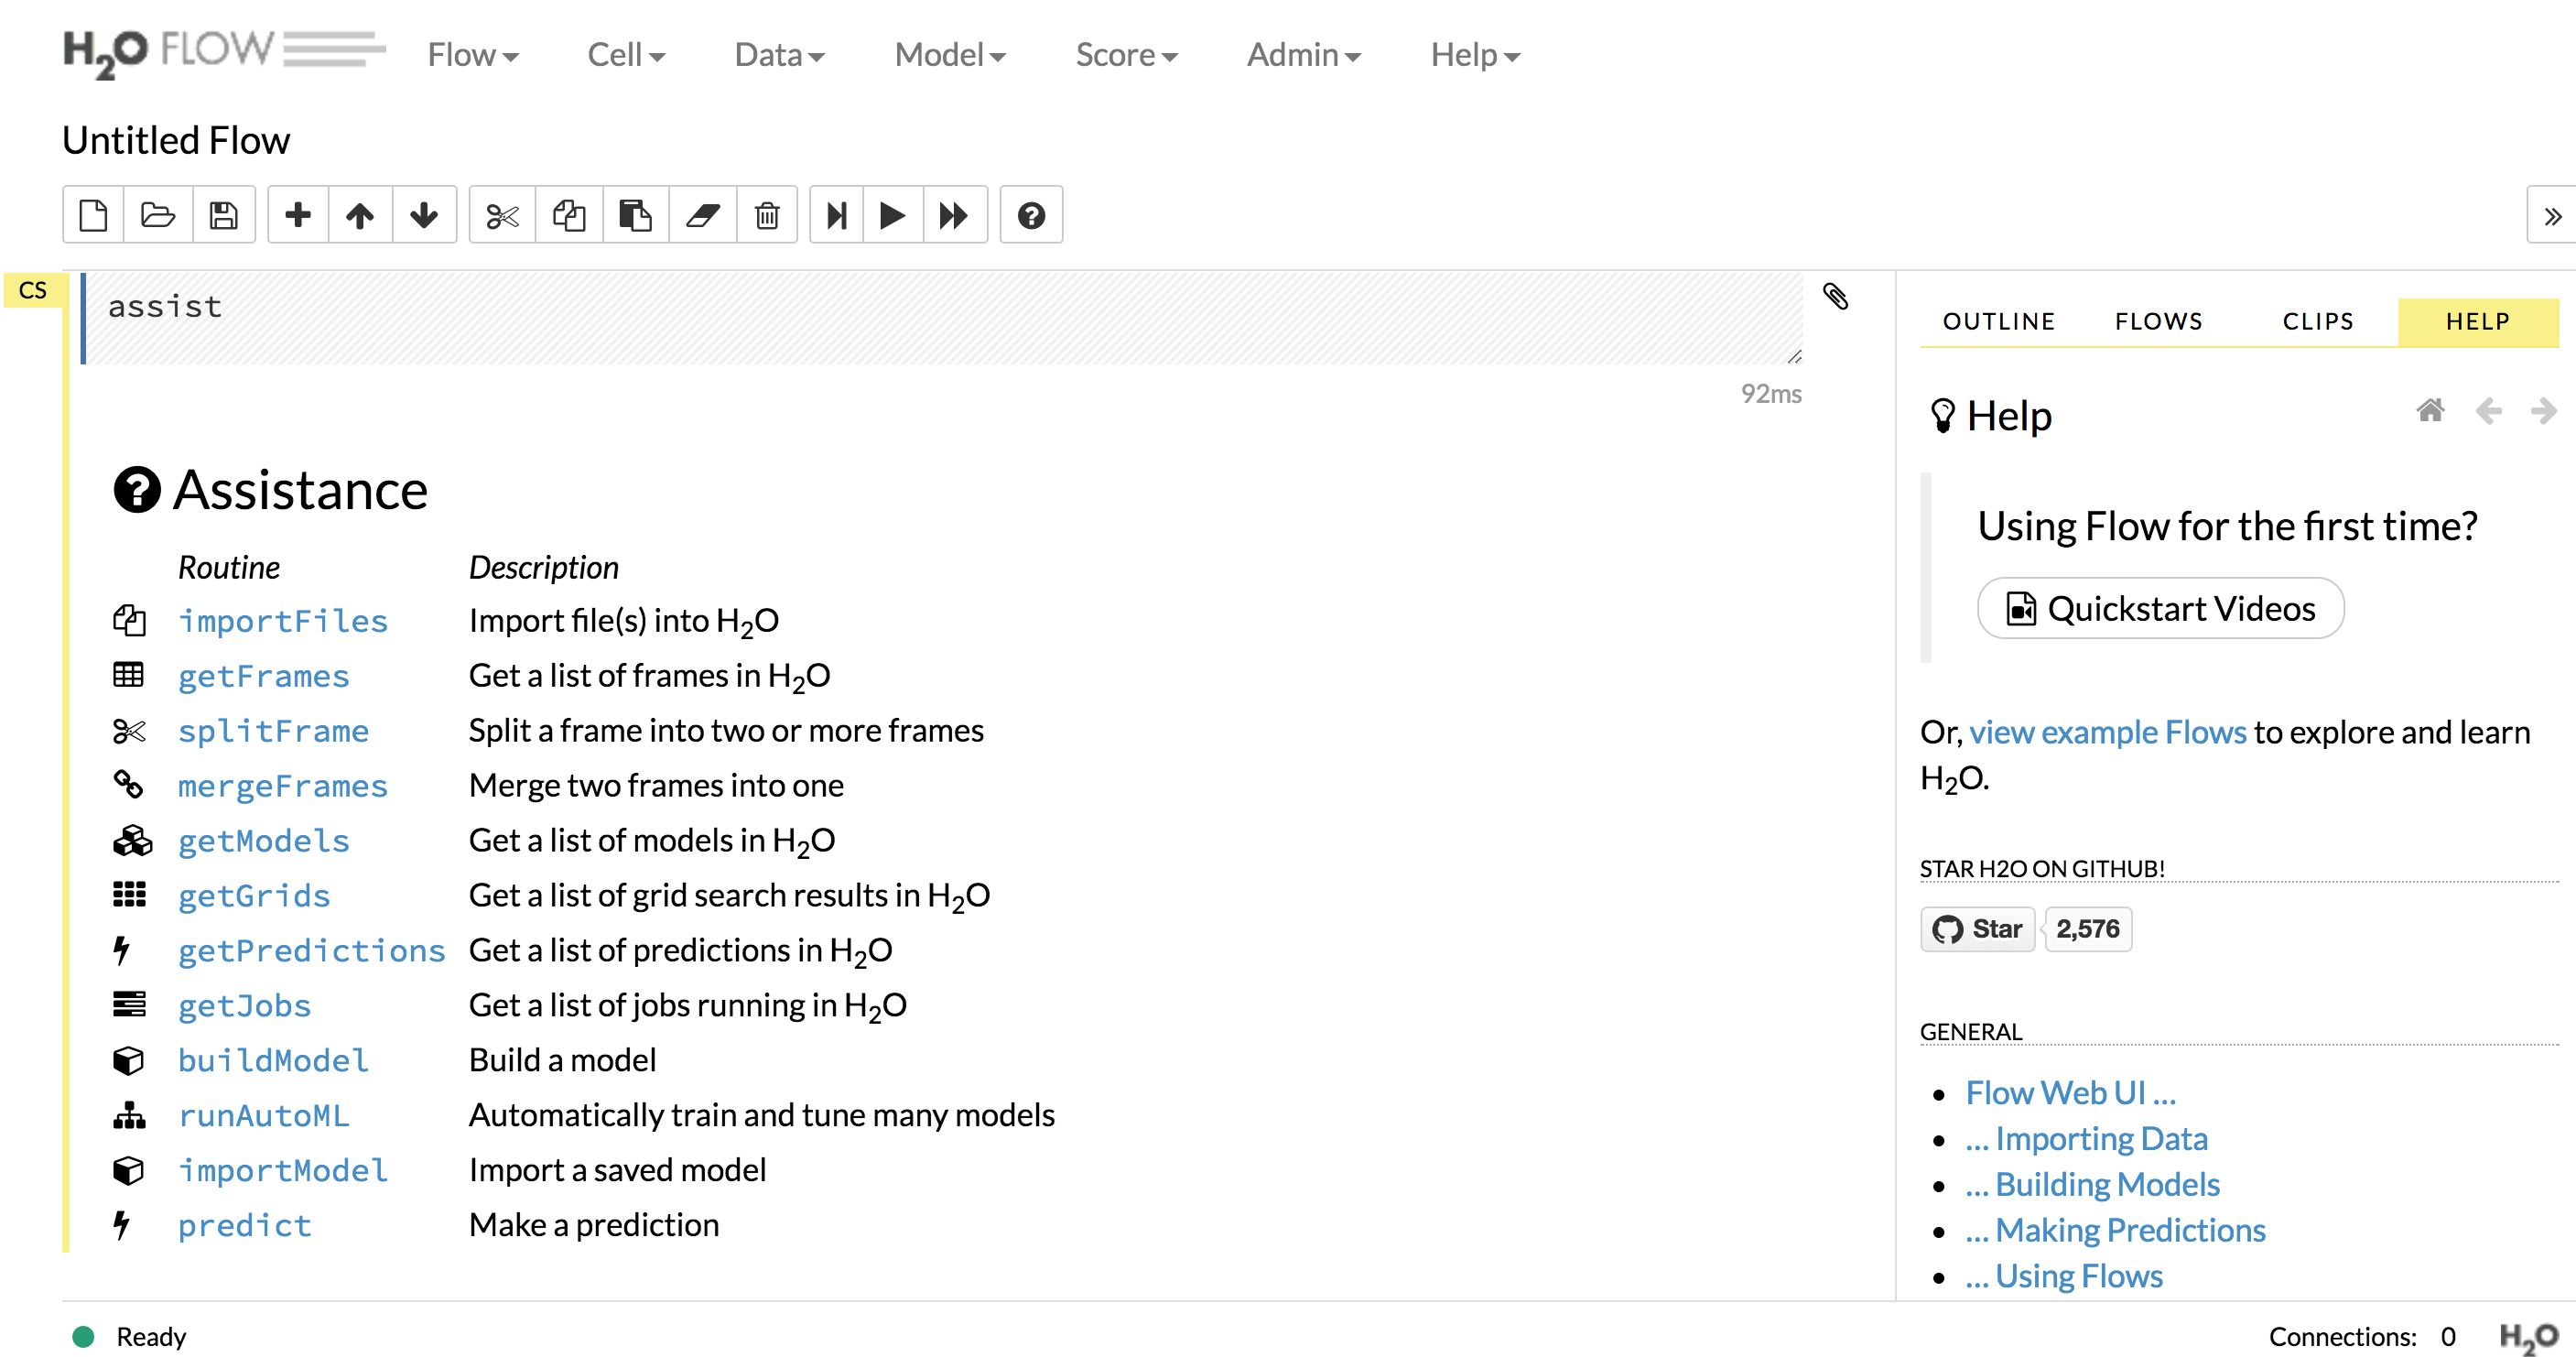
\includegraphics[width=39.08in]{images/ch6_h2o_flow} \end{center}

\subsection{Importing data into h2o from the R
session}\label{importing-data-into-h2o-from-the-r-session}

\begin{Shaded}
\begin{Highlighting}[]
\KeywordTok{data}\NormalTok{(cars)}
\NormalTok{cars_to_h2o <-}\StringTok{ }\KeywordTok{as.h2o}\NormalTok{(cars, }\DataTypeTok{destination_frame =} \StringTok{"cars_from_r"}\NormalTok{)}
\KeywordTok{is.data.frame}\NormalTok{(cars_to_h2o) }\CommentTok{# FALSE}
\KeywordTok{class}\NormalTok{(cars_to_h2o) }\CommentTok{# H2OFrame}
\end{Highlighting}
\end{Shaded}

(No persistence beyond the R session when h2O is started from R.)

\subsection{h2o functions}\label{h2o-functions}

\begin{Shaded}
\begin{Highlighting}[]
\KeywordTok{summary}\NormalTok{(cars_to_h2o) }\CommentTok{# actually calls h2o:::summary.H2OFrame(cars_to_h2o)}
\end{Highlighting}
\end{Shaded}

\begin{Shaded}
\begin{Highlighting}[]
\NormalTok{Approximated quantiles computed}\OperatorTok{!}\StringTok{ }\NormalTok{If you are interested }\ControlFlowTok{in}\NormalTok{ exact quantiles, please pass the }\StringTok{`}\DataTypeTok{exact_quantiles=TRUE}\StringTok{`}\NormalTok{ parameter. speed          dist            }
\NormalTok{ Min.   }\OperatorTok{:}\StringTok{ }\FloatTok{4.0}\NormalTok{   Min.   }\OperatorTok{:}\StringTok{  }\FloatTok{2.00}  
\NormalTok{ 1st Qu.}\OperatorTok{:}\FloatTok{12.0}\NormalTok{   1st Qu.}\OperatorTok{:}\StringTok{ }\FloatTok{26.00}  
\NormalTok{ Median }\OperatorTok{:}\FloatTok{15.0}\NormalTok{   Median }\OperatorTok{:}\StringTok{ }\FloatTok{36.00}  
\NormalTok{ Mean   }\OperatorTok{:}\FloatTok{15.4}\NormalTok{   Mean   }\OperatorTok{:}\StringTok{ }\FloatTok{42.98}  
\NormalTok{ 3rd Qu.}\OperatorTok{:}\FloatTok{19.0}\NormalTok{   3rd Qu.}\OperatorTok{:}\StringTok{ }\FloatTok{56.00}  
\NormalTok{ Max.   }\OperatorTok{:}\FloatTok{25.0}\NormalTok{   Max.   }\OperatorTok{:}\FloatTok{120.00}  
\end{Highlighting}
\end{Shaded}

\subsection{Let's check from the h2o
JVM}\label{lets-check-from-the-h2o-jvm}

From the browser: `Data' -\textgreater{} `List All Frames'

\begin{center}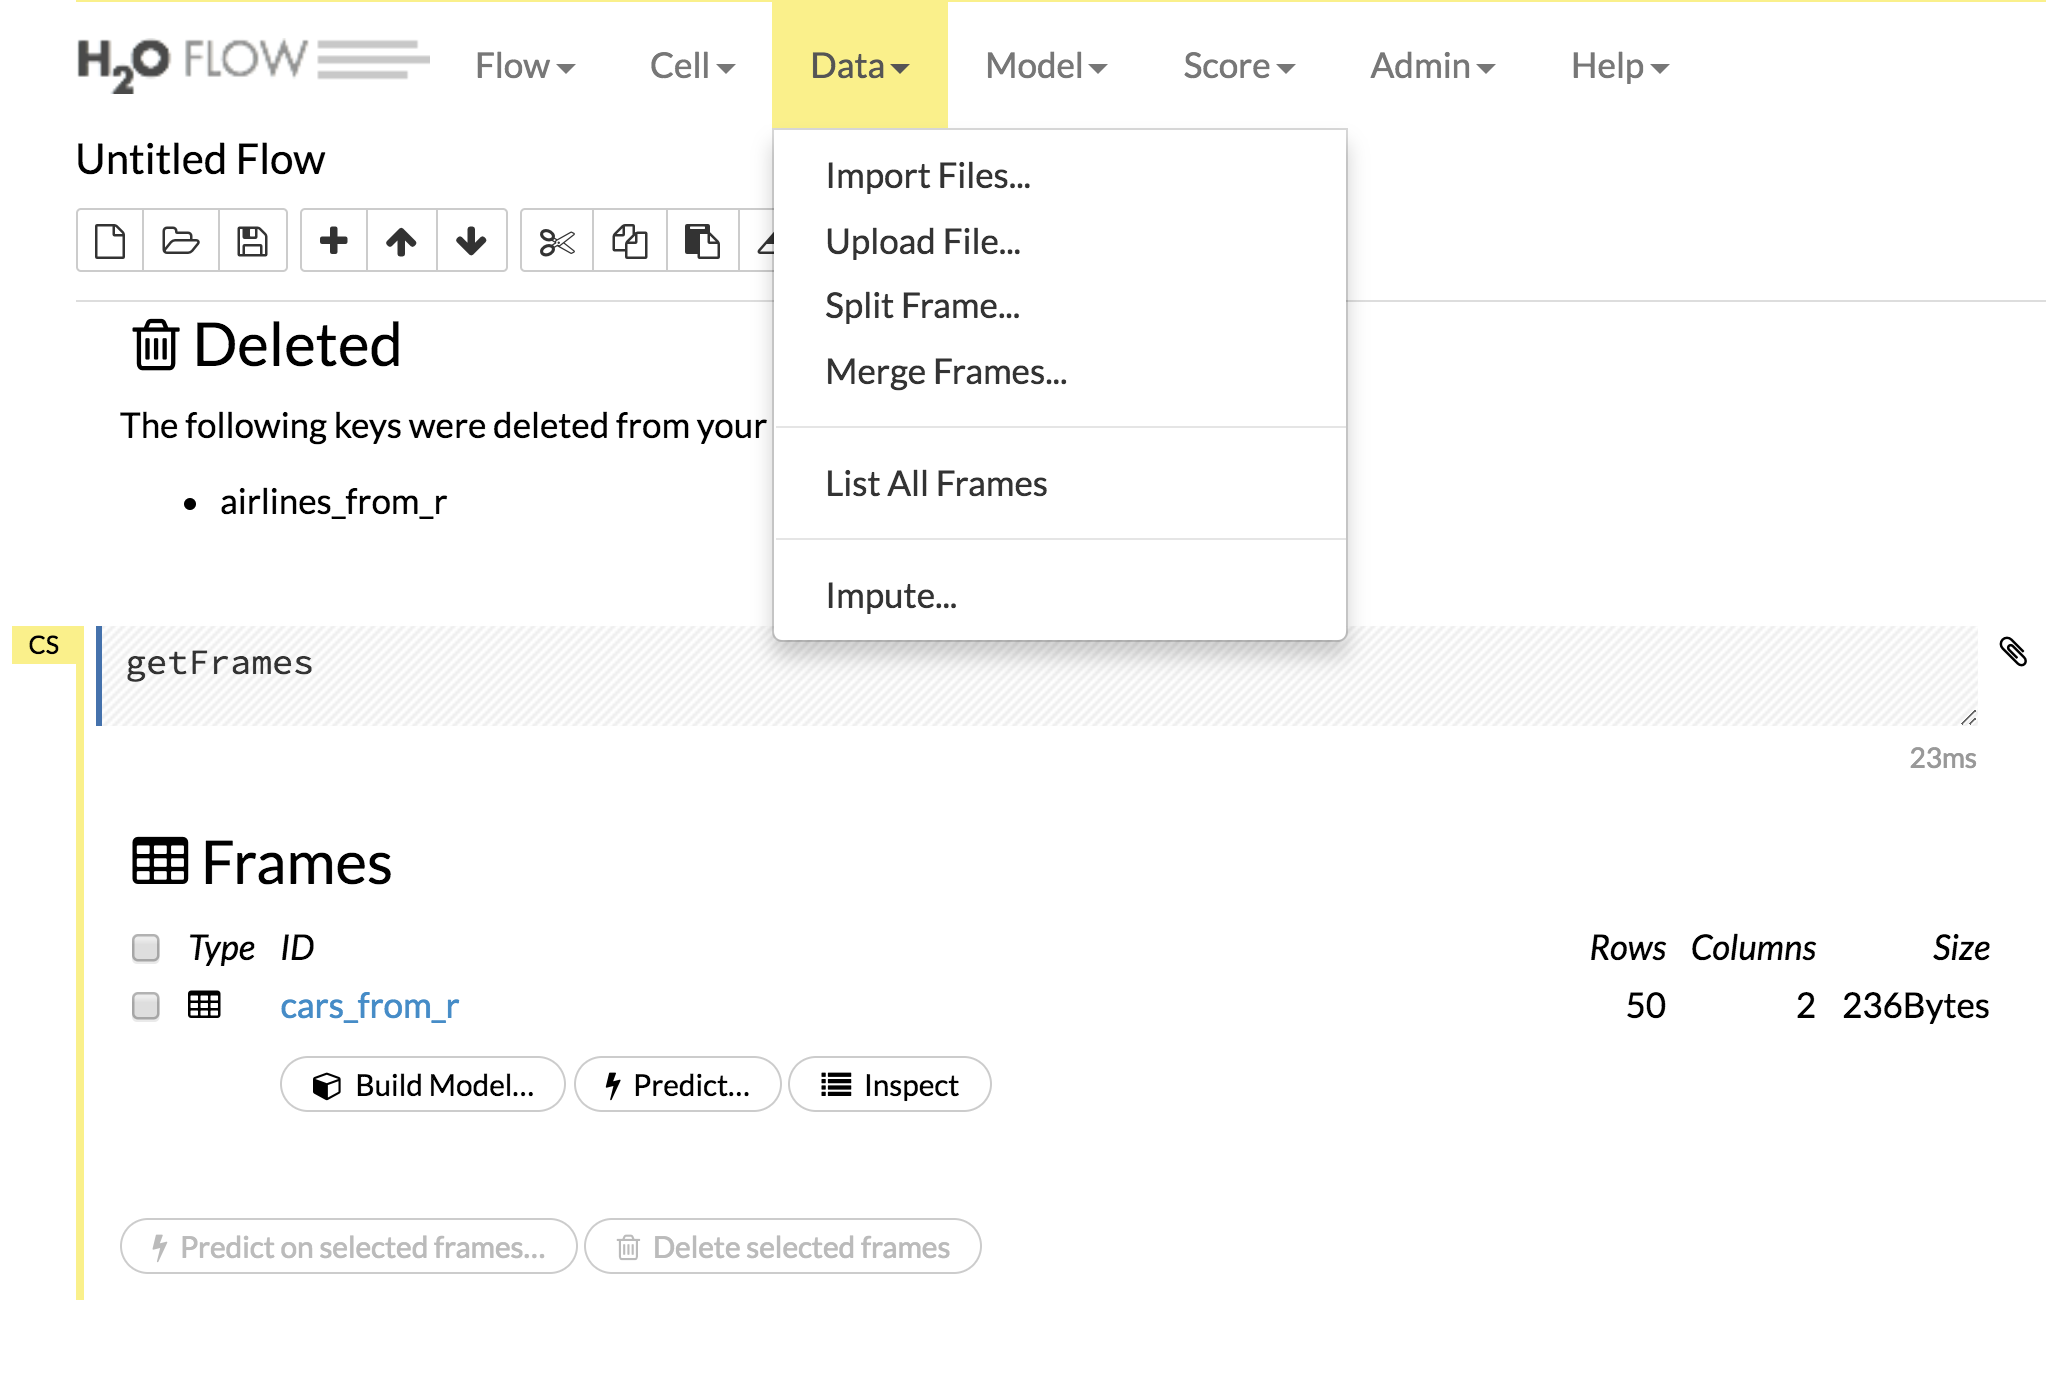
\includegraphics[width=28.42in]{images/ch6_h2o_list_data} \end{center}

\subsection{Importing data into h2o from
disk}\label{importing-data-into-h2o-from-disk}

\begin{Shaded}
\begin{Highlighting}[]
\NormalTok{airlines_path <-}\StringTok{ "/Users/cchoirat/Dropbox/Data17/AirFlights/allyears2k.csv"} \CommentTok{# full path}
\NormalTok{airlines_to_h2o <-}\StringTok{ }\KeywordTok{h2o.importFile}\NormalTok{(}\DataTypeTok{path =}\NormalTok{ airlines_path,}
                                  \DataTypeTok{destination_frame =} \StringTok{"airlines_from_r"}\NormalTok{)}
\KeywordTok{summary}\NormalTok{(airlines_to_h2o)}
\end{Highlighting}
\end{Shaded}

\subsection{Running a statistical
model}\label{running-a-statistical-model}

\begin{Shaded}
\begin{Highlighting}[]
\NormalTok{h2ofit <-}\StringTok{ }\KeywordTok{h2o.glm}\NormalTok{(}\DataTypeTok{y =} \StringTok{"ArrDelay"}\NormalTok{, }\DataTypeTok{x =} \StringTok{"Distance"}\NormalTok{,}
                  \DataTypeTok{training_frame =}\NormalTok{ airlines_to_h2o,}
                  \DataTypeTok{intercept =} \OtherTok{TRUE}\NormalTok{, }\CommentTok{# default is TRUE}
                  \DataTypeTok{family =} \StringTok{"gaussian"}\NormalTok{)}
\NormalTok{h2ofit}
\KeywordTok{summary}\NormalTok{(h2ofit)}
\end{Highlighting}
\end{Shaded}

\begin{Shaded}
\begin{Highlighting}[]
\NormalTok{Coefficients}\OperatorTok{:}\StringTok{ }\NormalTok{glm coefficients}
\NormalTok{      names coefficients standardized_coefficients}
\DecValTok{1}\NormalTok{ Intercept     }\FloatTok{7.702657}                  \FloatTok{9.308665}
\DecValTok{2}\NormalTok{  Distance     }\FloatTok{0.002199}                  \FloatTok{1.272253}
\end{Highlighting}
\end{Shaded}

\begin{Shaded}
\begin{Highlighting}[]
\NormalTok{airlines <-}\StringTok{ }\KeywordTok{read.csv}\NormalTok{(}\StringTok{"~/Dropbox/Data17/AirFlights/allyears2k.csv"}\NormalTok{)}
\NormalTok{rfit <-}\StringTok{ }\KeywordTok{lm}\NormalTok{(ArrDelay }\OperatorTok{~}\StringTok{ }\NormalTok{Distance, }\DataTypeTok{data =}\NormalTok{ airlines)}
\KeywordTok{summary}\NormalTok{(rfit)}
\end{Highlighting}
\end{Shaded}

\begin{Shaded}
\begin{Highlighting}[]
\NormalTok{Coefficients}\OperatorTok{:}
\StringTok{             }\NormalTok{Estimate Std. Error t value }\KeywordTok{Pr}\NormalTok{(}\OperatorTok{>}\ErrorTok{|}\NormalTok{t}\OperatorTok{|}\NormalTok{)    }
\NormalTok{(Intercept) }\FloatTok{7.7011553}  \FloatTok{0.2326198}  \FloatTok{33.106}   \OperatorTok{<}\FloatTok{2e-16} \OperatorTok{**}\ErrorTok{*}
\NormalTok{Distance    }\FloatTok{0.0022045}  \FloatTok{0.0002487}   \FloatTok{8.865}   \OperatorTok{<}\FloatTok{2e-16} \OperatorTok{**}\ErrorTok{*}
\end{Highlighting}
\end{Shaded}

\subsection{\texorpdfstring{\texttt{h2o}
models}{h2o models}}\label{h2o-models}

\begin{center}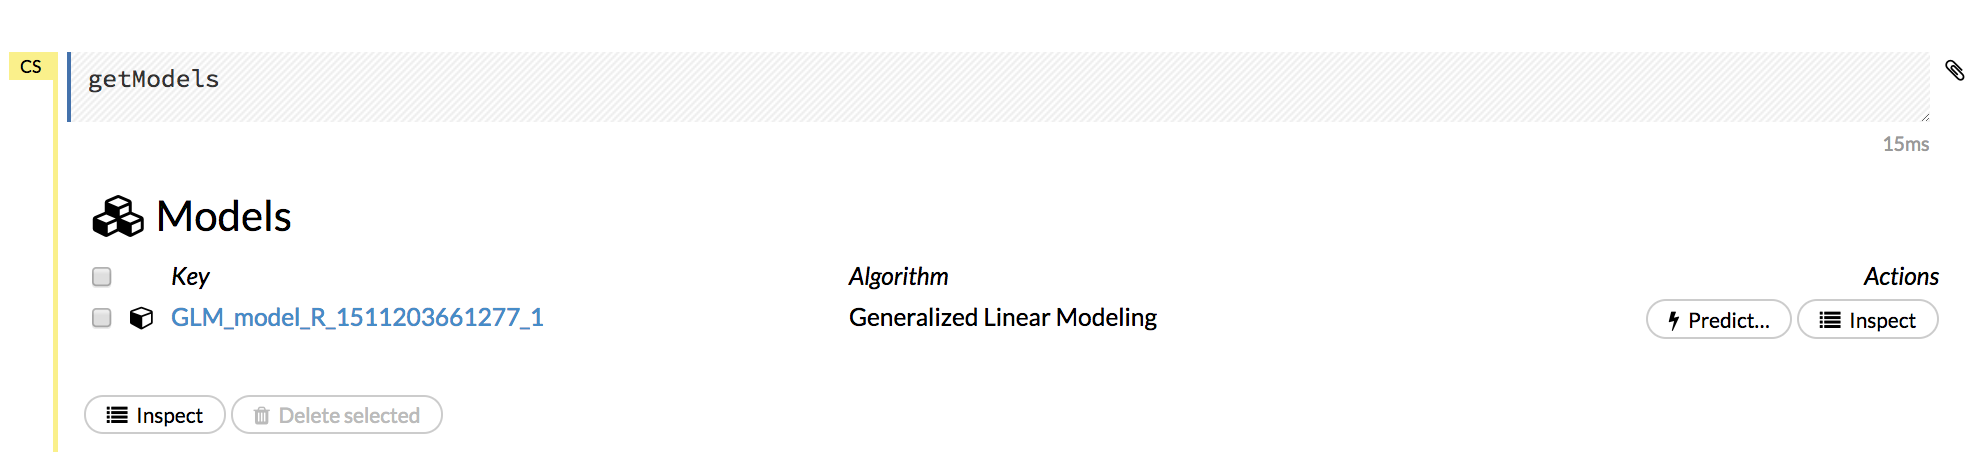
\includegraphics[width=27.51in]{images/ch6_h2o_models} \end{center}

\subsection{Closing the h2o session}\label{closing-the-h2o-session}

\begin{Shaded}
\begin{Highlighting}[]
\KeywordTok{h2o.shutdown}\NormalTok{()}
\end{Highlighting}
\end{Shaded}

\subsection{Available algorithms}\label{available-algorithms}

\begin{itemize}
\tightlist
\item
  Deep learning
\item
  Distributed randon forest
\item
  Gradient boosting method
\item
  Generalized linear modeling
\item
  Generalized low rank modeling
\item
  K-means
\item
  Naive Bayes
\item
  Principal component analysis
\end{itemize}

\subsection{How to incorporate new models in
h2o?}\label{how-to-incorporate-new-models-in-h2o}

\textbf{(+)} built-in models behave very much like R and are scalable

\textbf{(-)} not easy to extend (\emph{e.g}., GLM
\url{https://github.com/h2oai/h2o-3/blob/master/h2o-algos/src/main/java/hex/glm/GLM.java})

\BeginKnitrBlock{exercise}
\protect\hypertarget{exr:unnamed-chunk-140}{}{\label{exr:unnamed-chunk-140}
}Run the same analysis with the whole dataset \texttt{allyears.csv}.
\EndKnitrBlock{exercise}

\section{Spark}\label{spark}

Reading: \url{https://spark.rstudio.com/}

\begin{Shaded}
\begin{Highlighting}[]
\KeywordTok{library}\NormalTok{(sparklyr)}
\KeywordTok{spark_install}\NormalTok{(}\DataTypeTok{version =} \StringTok{"2.1.0"}\NormalTok{)}
\end{Highlighting}
\end{Shaded}

\begin{Shaded}
\begin{Highlighting}[]
\NormalTok{conf <-}\StringTok{ }\KeywordTok{spark_config}\NormalTok{()}
\NormalTok{conf}\OperatorTok{$}\StringTok{`}\DataTypeTok{sparklyr.shell.driver-memory}\StringTok{`}\NormalTok{ <-}\StringTok{ "32G"}
\NormalTok{conf}\OperatorTok{$}\NormalTok{spark.memory.fraction <-}\StringTok{ }\FloatTok{0.5}
\NormalTok{sc <-}\StringTok{ }\KeywordTok{spark_connect}\NormalTok{(}\DataTypeTok{master =} \StringTok{"local"}\NormalTok{)}
\end{Highlighting}
\end{Shaded}

\begin{Shaded}
\begin{Highlighting}[]
\KeywordTok{library}\NormalTok{(dplyr)}
\NormalTok{iris_tbl <-}\StringTok{ }\KeywordTok{copy_to}\NormalTok{(sc, iris)}
\NormalTok{flights_tbl <-}\StringTok{ }\KeywordTok{copy_to}\NormalTok{(sc, nycflights13}\OperatorTok{::}\NormalTok{flights, }\StringTok{"flights"}\NormalTok{)}
\NormalTok{batting_tbl <-}\StringTok{ }\KeywordTok{copy_to}\NormalTok{(sc, Lahman}\OperatorTok{::}\NormalTok{Batting, }\StringTok{"batting"}\NormalTok{)}
\KeywordTok{src_tbls}\NormalTok{(sc)}
\end{Highlighting}
\end{Shaded}

\begin{Shaded}
\begin{Highlighting}[]
\NormalTok{[}\DecValTok{1}\NormalTok{] }\StringTok{"batting"} \StringTok{"flights"} \StringTok{"iris"}
\end{Highlighting}
\end{Shaded}

You can use SQL:

\begin{Shaded}
\begin{Highlighting}[]
\KeywordTok{library}\NormalTok{(DBI)}
\NormalTok{iris_preview <-}\StringTok{ }\KeywordTok{dbGetQuery}\NormalTok{(sc, }\StringTok{"SELECT * FROM iris LIMIT 10"}\NormalTok{)}
\end{Highlighting}
\end{Shaded}

Like h2o, you can open a web interface:

\begin{Shaded}
\begin{Highlighting}[]
\KeywordTok{spark_web}\NormalTok{(sc)}
\end{Highlighting}
\end{Shaded}

\begin{Shaded}
\begin{Highlighting}[]
\NormalTok{top_rows <-}\StringTok{ }\KeywordTok{read.csv}\NormalTok{(}\StringTok{"~/Dropbox/Data17/AirFlights/allyears.csv"}\NormalTok{, }\DataTypeTok{nrows =} \DecValTok{5}\NormalTok{)}
\NormalTok{file_columns <-}\StringTok{ }\NormalTok{top_rows }\OperatorTok\StringTok{ }
\StringTok{  }\NormalTok{purrr}\OperatorTok{::}\KeywordTok{map}\NormalTok{(}\ControlFlowTok{function}\NormalTok{(x)}\StringTok{"character"}\NormalTok{)}
\KeywordTok{rm}\NormalTok{(top_rows)}
\end{Highlighting}
\end{Shaded}

\begin{Shaded}
\begin{Highlighting}[]
\NormalTok{sp_flights <-}\StringTok{ }\KeywordTok{spark_read_csv}\NormalTok{(sc, }
                             \DataTypeTok{name =} \StringTok{"flights2"}\NormalTok{, }
                             \DataTypeTok{path =} \StringTok{"~/Dropbox/Data17/AirFlights/allyears.csv"}\NormalTok{, }
                             \DataTypeTok{memory =} \OtherTok{FALSE}\NormalTok{, }
                             \DataTypeTok{columns =}\NormalTok{ file_columns, }
                             \DataTypeTok{infer_schema =} \OtherTok{FALSE}\NormalTok{)}
\end{Highlighting}
\end{Shaded}

\begin{Shaded}
\begin{Highlighting}[]
\CommentTok{# Source:   table<flights2> [?? x 31]}
\CommentTok{# Database: spark_connection}
\NormalTok{    Year Month DayofMonth DayOfWeek DepTime CRSDepTime ArrTime CRSArrTime UniqueCarrier}
   \OperatorTok{<}\NormalTok{chr}\OperatorTok{>}\StringTok{ }\ErrorTok{<}\NormalTok{chr}\OperatorTok{>}\StringTok{      }\ErrorTok{<}\NormalTok{chr}\OperatorTok{>}\StringTok{     }\ErrorTok{<}\NormalTok{chr}\OperatorTok{>}\StringTok{   }\ErrorTok{<}\NormalTok{chr}\OperatorTok{>}\StringTok{      }\ErrorTok{<}\NormalTok{chr}\OperatorTok{>}\StringTok{   }\ErrorTok{<}\NormalTok{chr}\OperatorTok{>}\StringTok{      }\ErrorTok{<}\NormalTok{chr}\OperatorTok{>}\StringTok{         }\ErrorTok{<}\NormalTok{chr}\OperatorTok{>}
\StringTok{ }\DecValTok{1}  \DecValTok{1987}    \DecValTok{10}         \DecValTok{14}         \DecValTok{3}     \DecValTok{741}        \DecValTok{730}     \DecValTok{912}        \DecValTok{849}\NormalTok{            PS}
 \DecValTok{2}  \DecValTok{1987}    \DecValTok{10}         \DecValTok{15}         \DecValTok{4}     \DecValTok{729}        \DecValTok{730}     \DecValTok{903}        \DecValTok{849}\NormalTok{            PS}
 \DecValTok{3}  \DecValTok{1987}    \DecValTok{10}         \DecValTok{17}         \DecValTok{6}     \DecValTok{741}        \DecValTok{730}     \DecValTok{918}        \DecValTok{849}\NormalTok{            PS}
 \DecValTok{4}  \DecValTok{1987}    \DecValTok{10}         \DecValTok{18}         \DecValTok{7}     \DecValTok{729}        \DecValTok{730}     \DecValTok{847}        \DecValTok{849}\NormalTok{            PS}
 \DecValTok{5}  \DecValTok{1987}    \DecValTok{10}         \DecValTok{19}         \DecValTok{1}     \DecValTok{749}        \DecValTok{730}     \DecValTok{922}        \DecValTok{849}\NormalTok{            PS}
 \DecValTok{6}  \DecValTok{1987}    \DecValTok{10}         \DecValTok{21}         \DecValTok{3}     \DecValTok{728}        \DecValTok{730}     \DecValTok{848}        \DecValTok{849}\NormalTok{            PS}
 \DecValTok{7}  \DecValTok{1987}    \DecValTok{10}         \DecValTok{22}         \DecValTok{4}     \DecValTok{728}        \DecValTok{730}     \DecValTok{852}        \DecValTok{849}\NormalTok{            PS}
 \DecValTok{8}  \DecValTok{1987}    \DecValTok{10}         \DecValTok{23}         \DecValTok{5}     \DecValTok{731}        \DecValTok{730}     \DecValTok{902}        \DecValTok{849}\NormalTok{            PS}
 \DecValTok{9}  \DecValTok{1987}    \DecValTok{10}         \DecValTok{24}         \DecValTok{6}     \DecValTok{744}        \DecValTok{730}     \DecValTok{908}        \DecValTok{849}\NormalTok{            PS}
\DecValTok{10}  \DecValTok{1987}    \DecValTok{10}         \DecValTok{25}         \DecValTok{7}     \DecValTok{729}        \DecValTok{730}     \DecValTok{851}        \DecValTok{849}\NormalTok{            PS}
\CommentTok{# ... with more rows, and 22 more variables: FlightNum <chr>, TailNum <chr>,}
\CommentTok{#   ActualElapsedTime <chr>, CRSElapsedTime <chr>, AirTime <chr>, ArrDelay <chr>,}
\CommentTok{#   DepDelay <chr>, Origin <chr>, Dest <chr>, Distance <chr>, TaxiIn <chr>,}
\CommentTok{#   TaxiOut <chr>, Cancelled <chr>, CancellationCode <chr>, Diverted <chr>,}
\CommentTok{#   CarrierDelay <chr>, WeatherDelay <chr>, NASDelay <chr>, SecurityDelay <chr>,}
\CommentTok{#   LateAircraftDelay <chr>, IsArrDelayed <chr>, IsDepDelayed <chr>}
\end{Highlighting}
\end{Shaded}

\begin{Shaded}
\begin{Highlighting}[]
\NormalTok{flights_table <-}\StringTok{ }\NormalTok{sp_flights }\OperatorTok
\StringTok{  }\KeywordTok{mutate}\NormalTok{(}\DataTypeTok{DepDelay =} \KeywordTok{as.numeric}\NormalTok{(DepDelay),}
         \DataTypeTok{ArrDelay =} \KeywordTok{as.numeric}\NormalTok{(ArrDelay),}
         \DataTypeTok{Distance =} \KeywordTok{as.numeric}\NormalTok{(Distance),}
         \DataTypeTok{SchedDeparture =} \KeywordTok{as.numeric}\NormalTok{(CRSDepTime)) }\OperatorTok
\StringTok{  }\KeywordTok{select}\NormalTok{(Origin, Dest, SchedDeparture, ArrDelay, DepDelay, Month, DayofMonth, Distance)}

\NormalTok{flights_table }\OperatorTok\StringTok{ }\NormalTok{head}
\end{Highlighting}
\end{Shaded}

Cache data:

\begin{Shaded}
\begin{Highlighting}[]
\NormalTok{sp_flights }\OperatorTok
\StringTok{  }\NormalTok{tally }\CommentTok{# takes a looooong time}
\end{Highlighting}
\end{Shaded}

123534969\ldots{}

\begin{Shaded}
\begin{Highlighting}[]
\CommentTok{# might take a while...}
\NormalTok{subset_table <-}\StringTok{ }\NormalTok{flights_table }\OperatorTok\StringTok{ }
\StringTok{  }\KeywordTok{compute}\NormalTok{(}\StringTok{"flights_subset"}\NormalTok{)}
\end{Highlighting}
\end{Shaded}

\begin{Shaded}
\begin{Highlighting}[]
\NormalTok{subset_table }\OperatorTok
\StringTok{  }\NormalTok{tally }\CommentTok{# a bit faster.}
\end{Highlighting}
\end{Shaded}

123534969 as well!

\subsection{Run a statistical model}\label{run-a-statistical-model}

\begin{Shaded}
\begin{Highlighting}[]
\CommentTok{# small_flights <- spark_read_csv(sc, }
\CommentTok{#                              name = "flights2", }
\CommentTok{#                              path = "~/Dropbox/Data17/AirFlights/allyears2k.csv", }
\CommentTok{#                              memory = FALSE, }
\CommentTok{#                              columns = file_columns, }
\CommentTok{#                              infer_schema = FALSE)}
\end{Highlighting}
\end{Shaded}

\begin{Shaded}
\begin{Highlighting}[]
\CommentTok{# small_flights_table <- small_flights %>%}
\CommentTok{#   mutate(DepDelay = as.numeric(DepDelay),}
\CommentTok{#          ArrDelay = as.numeric(ArrDelay),}
\CommentTok{#          Distance = as.numeric(Distance),}
\CommentTok{#          SchedDeparture = as.numeric(CRSDepTime)) %>%}
\CommentTok{#   select(Origin, Dest, SchedDeparture, ArrDelay, DepDelay, Month, DayofMonth, Distance)}
\CommentTok{# }
\CommentTok{# small_flights_table %>% head}
\end{Highlighting}
\end{Shaded}

\begin{Shaded}
\begin{Highlighting}[]
\CommentTok{# lm(arr_delay ~ distance, data = flights_tbl)}
 \KeywordTok{ml_linear_regression}\NormalTok{(flights_table, }\DataTypeTok{response =} \StringTok{"ArrDelay"}\NormalTok{, }\DataTypeTok{features =} \StringTok{"Distance"}\NormalTok{)}
\end{Highlighting}
\end{Shaded}

\begin{Shaded}
\begin{Highlighting}[]
\NormalTok{Coefficients}\OperatorTok{:}
\StringTok{ }\NormalTok{(Intercept)     Distance }
\FloatTok{6.9707048955} \FloatTok{0.0001100521}
\end{Highlighting}
\end{Shaded}

\begin{figure}

{\centering 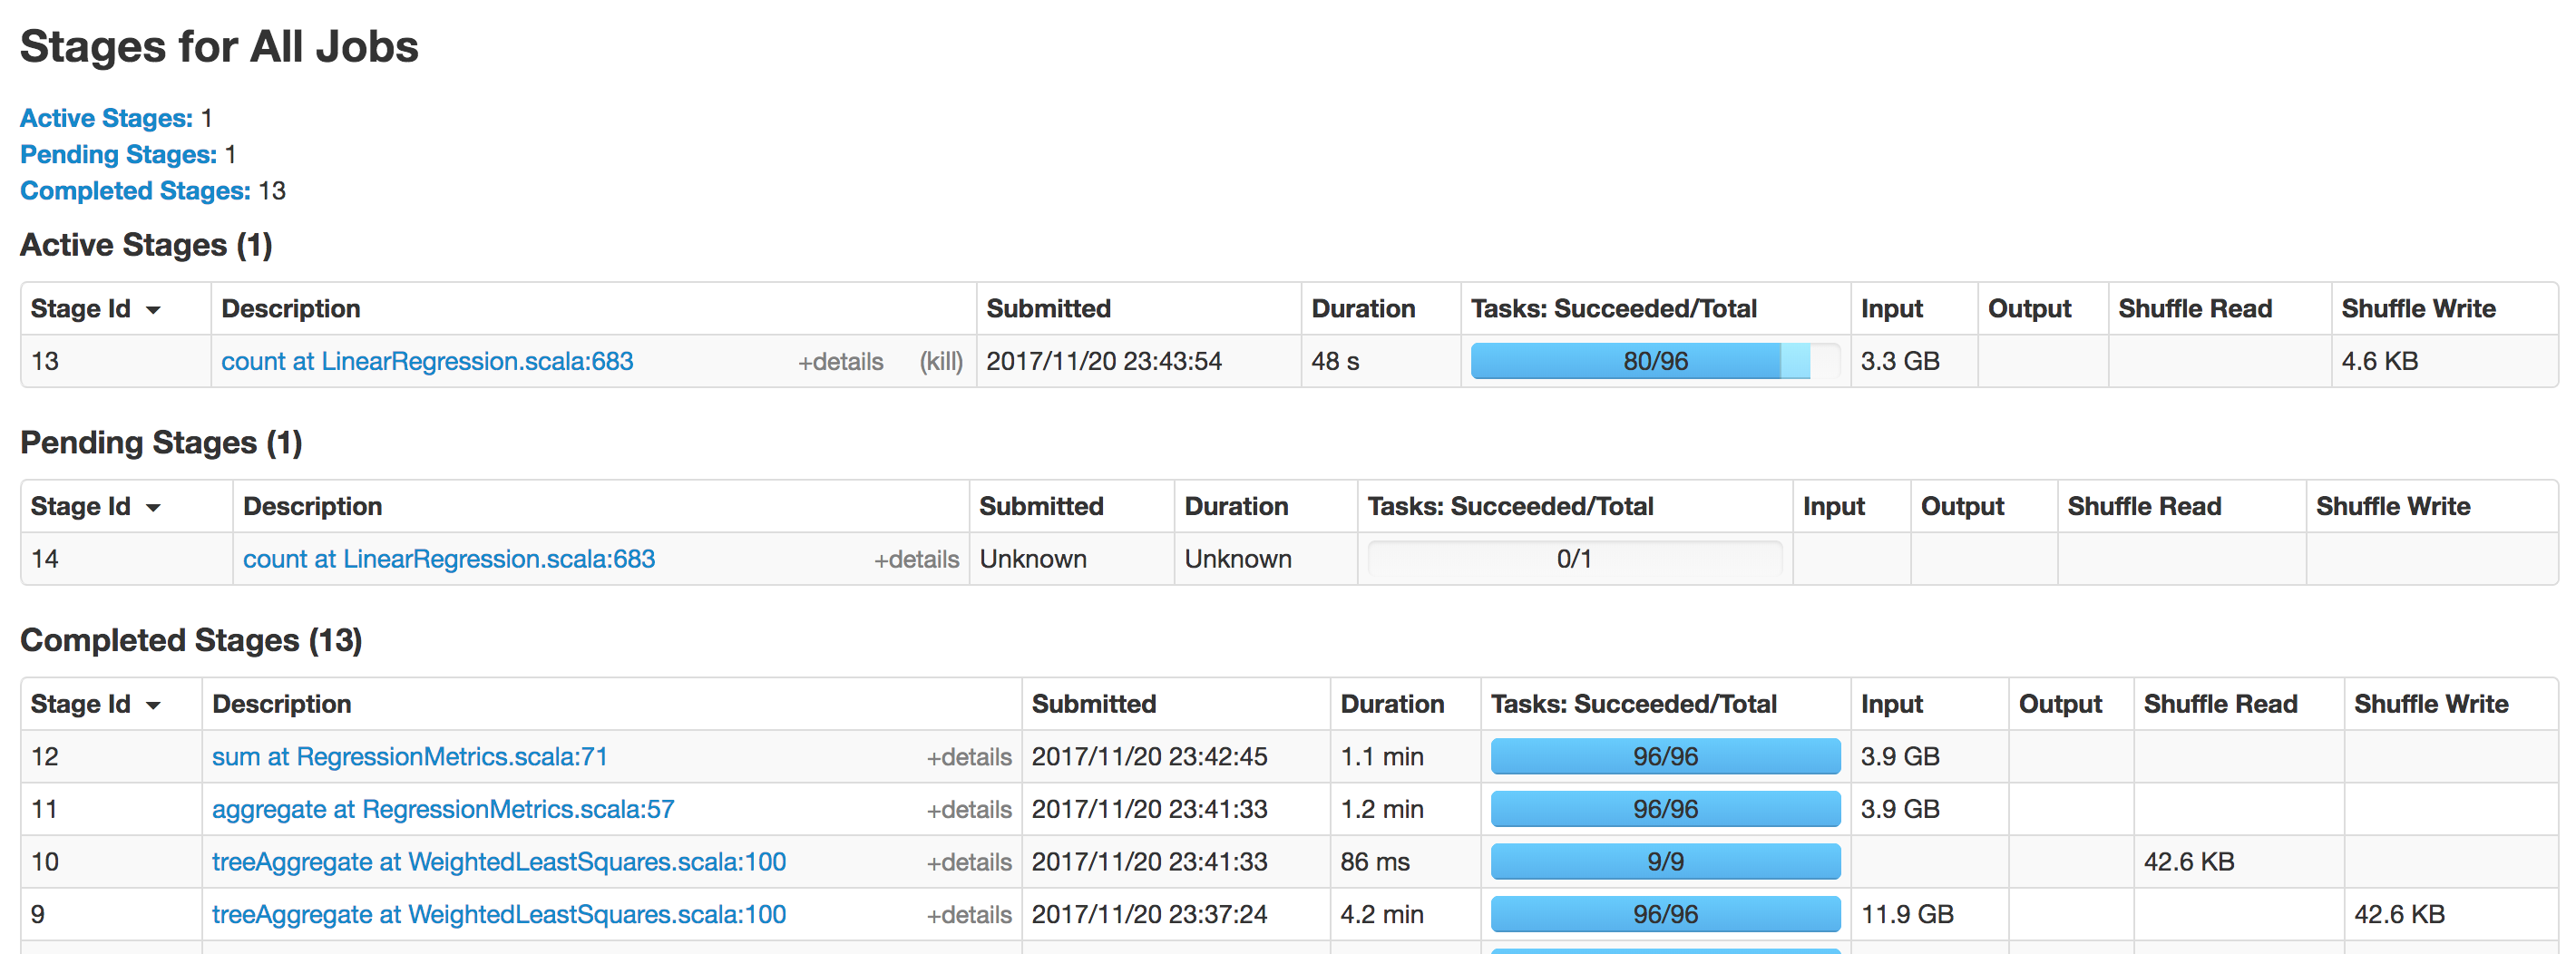
\includegraphics[width=39.44in]{images/ch6_spark_jobs} 

}

\end{figure}

\subsection{Deployment}\label{deployment}

Reading: \url{https://spark.rstudio.com/deployment.html}

\section{\texorpdfstring{\texttt{Sparkling\ Water}}{Sparkling Water}}\label{sparkling-water}

Reading: \url{https://spark.rstudio.com/h2o.html}

\section{\texorpdfstring{Adding new models to \texttt{h2o} and
\texttt{spark}}{Adding new models to h2o and spark}}\label{adding-new-models-to-h2o-and-spark}

\section{More?}\label{more}

GPU

\section{Amazon Web Services (AWS)}\label{amazon-web-services-aws}

AWS Management Console: \url{https://aws.amazon.com/console/}

\begin{itemize}
\tightlist
\item
  Amazon EC2
\end{itemize}

\begin{quote}
Amazon Elastic Compute Cloud (Amazon EC2) is a web service that provides
secure, resizable compute capacity in the cloud. It is designed to make
web-scale cloud computing easier for developers.
\end{quote}

Let's launch an \texttt{Amazon\ Linux} instance (\texttt{t2.micro} free
tier eligible) and configure a security group (Custom TCP, port 8787).

\begin{figure}

{\centering 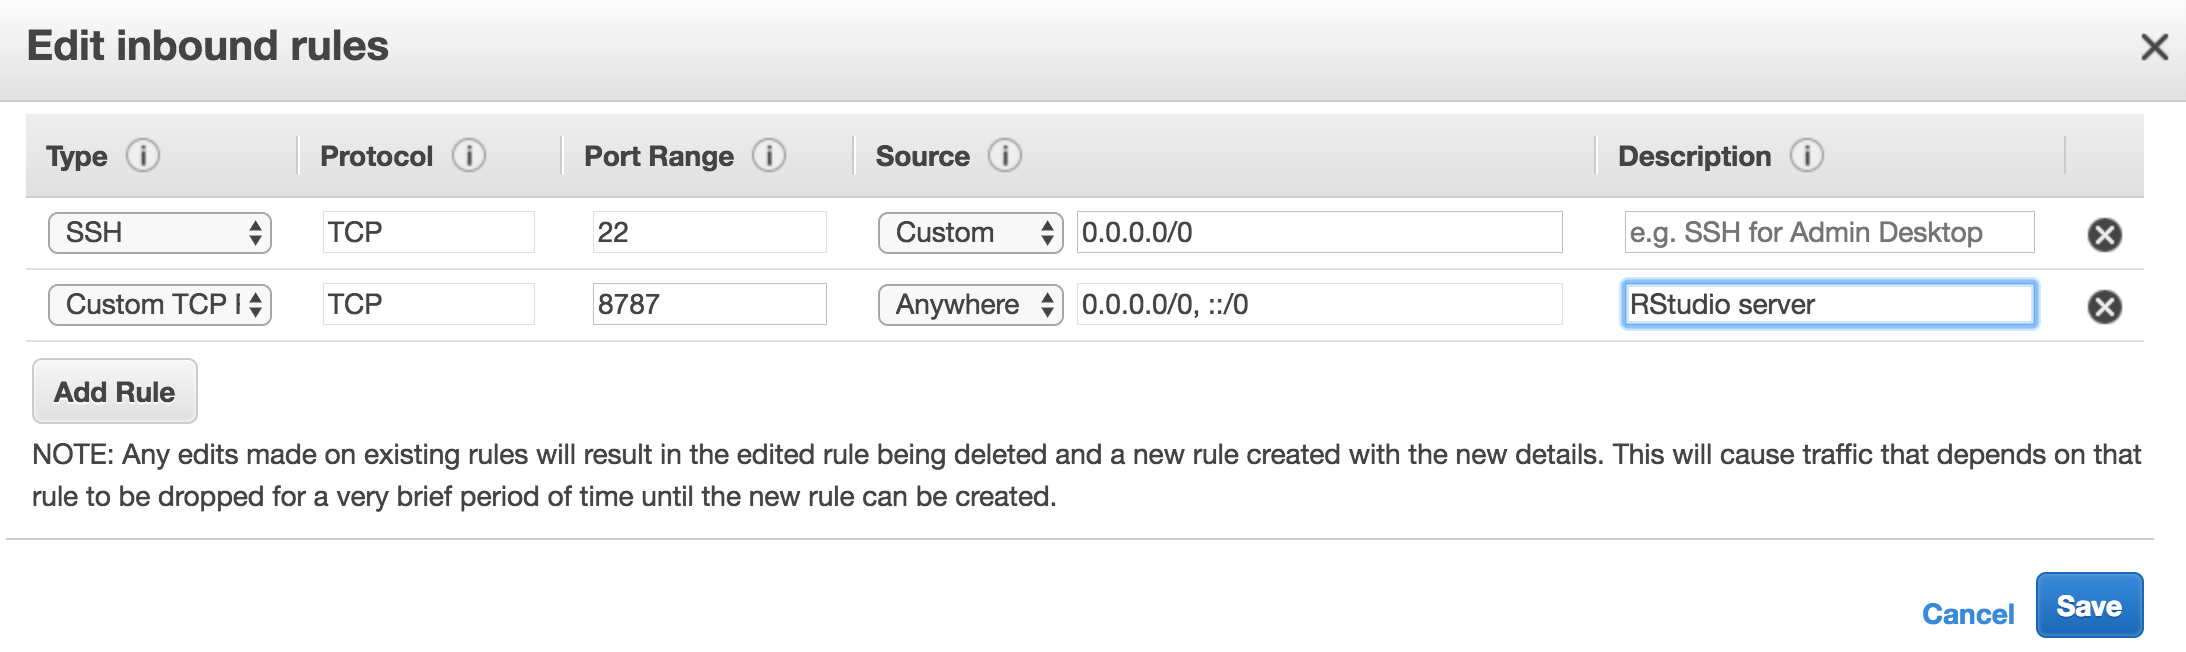
\includegraphics[width=30.36in]{images/ch6_aws_security_groups} 

}

\end{figure}

To connect:

\begin{Shaded}
\begin{Highlighting}[]
\NormalTok{chmod }\DecValTok{400} \OperatorTok{~}\ErrorTok{/}\NormalTok{Downloads}\OperatorTok{/}\NormalTok{bst262}\OperatorTok{-}\NormalTok{demo.pem}
\NormalTok{ssh }\OperatorTok{-}\NormalTok{i }\StringTok{"~/Downloads/bst262-demo.pem"}\NormalTok{ ec2}\OperatorTok{-}\NormalTok{user}\OperatorTok{@}\NormalTok{ec2}\OperatorTok{-}\DecValTok{18}\OperatorTok{-}\DecValTok{217}\OperatorTok{-}\DecValTok{97}\OperatorTok{-}\FloatTok{206.}\NormalTok{us}\OperatorTok{-}\NormalTok{east}\OperatorTok{-}\FloatTok{2.}\NormalTok{compute.amazonaws.com}
\end{Highlighting}
\end{Shaded}

\begin{verbatim}

       __|  __|_  )
       _|  (     /   Amazon Linux AMI
      ___|\___|___|
\end{verbatim}

We install \texttt{R}

\begin{Shaded}
\begin{Highlighting}[]
\NormalTok{sudo yum update}
\NormalTok{sudo yum list R}\OperatorTok{-}\NormalTok{\textbackslash{}}\OperatorTok{*}
\NormalTok{sudo yum install R}
\end{Highlighting}
\end{Shaded}

and \texttt{Rstudio\ server} (\#
\url{https://www.rstudio.com/products/rstudio/download-server/})

\begin{Shaded}
\begin{Highlighting}[]
\NormalTok{wget https}\OperatorTok{:}\ErrorTok{//}\NormalTok{download2.rstudio.org}\OperatorTok{/}\NormalTok{rstudio}\OperatorTok{-}\NormalTok{server}\OperatorTok{-}\NormalTok{rhel}\OperatorTok{-}\FloatTok{1.1}\NormalTok{.}\DecValTok{383}\OperatorTok{-}\NormalTok{x86_}\FloatTok{64.}\NormalTok{rpm}
\NormalTok{sudo yum install }\OperatorTok{--}\NormalTok{nogpgcheck rstudio}\OperatorTok{-}\NormalTok{server}\OperatorTok{-}\NormalTok{rhel}\OperatorTok{-}\FloatTok{1.1}\NormalTok{.}\DecValTok{383}\OperatorTok{-}\NormalTok{x86_}\FloatTok{64.}\NormalTok{rpm}
\end{Highlighting}
\end{Shaded}

We need to add user and password:

\begin{Shaded}
\begin{Highlighting}[]
\NormalTok{sudo useradd rserver}
\NormalTok{sudo passwd rserver}
\end{Highlighting}
\end{Shaded}

RStudio server uses port 8787. Let's fix the security groups:

\begin{figure}

{\centering 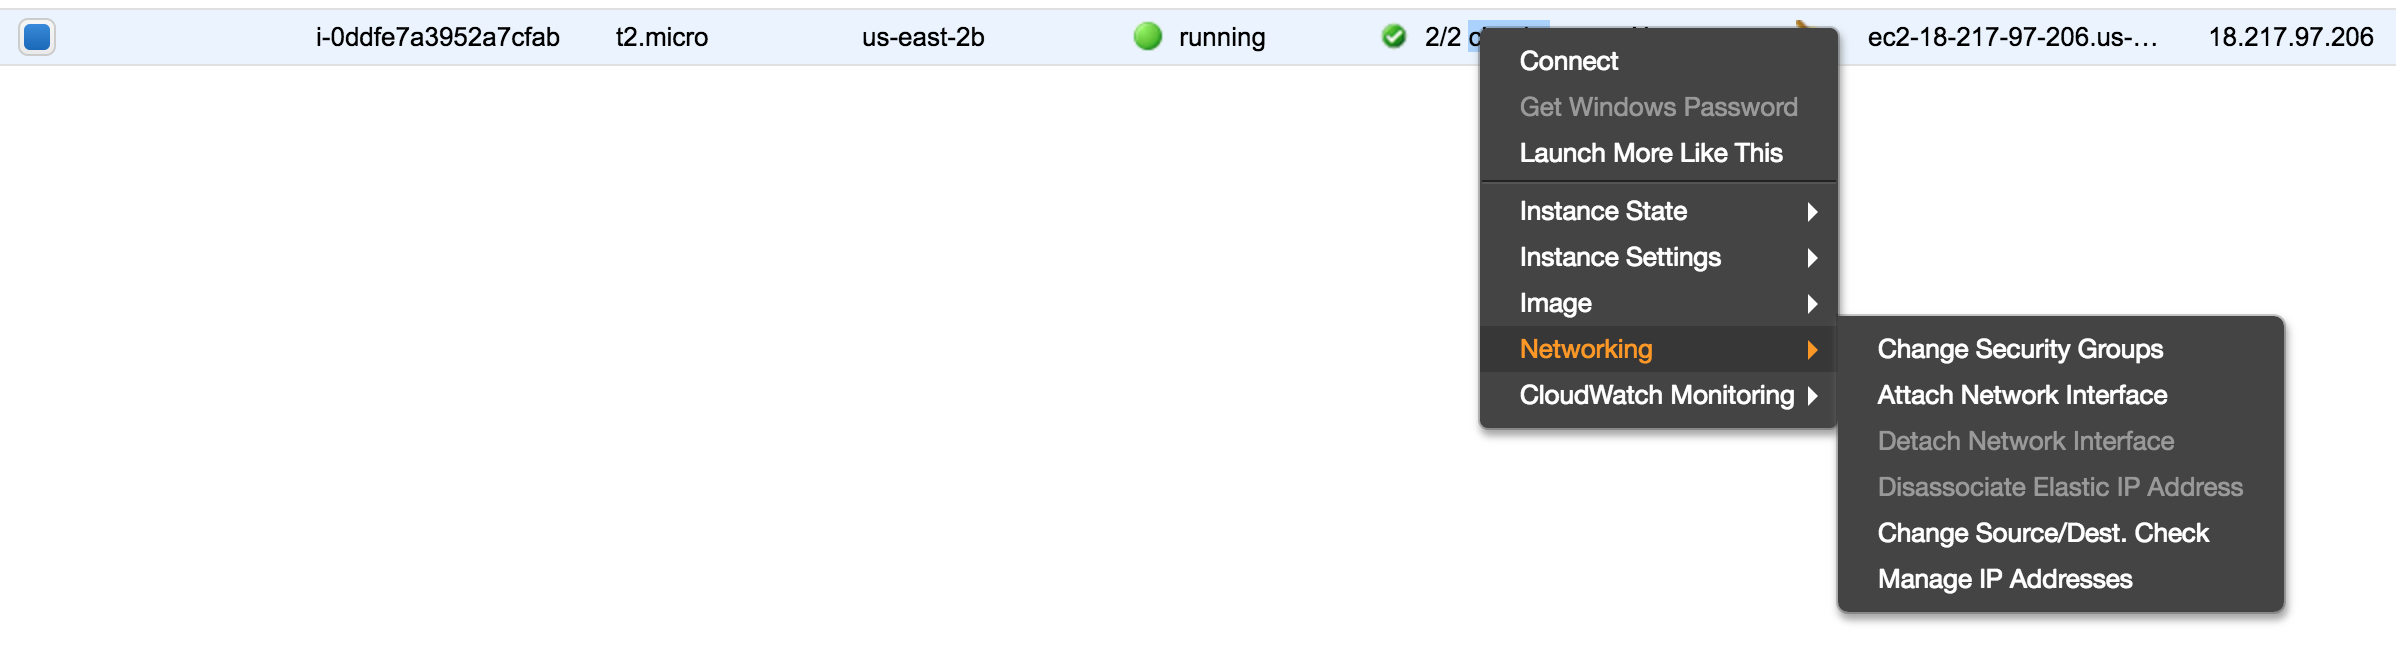
\includegraphics[width=33.28in]{images/ch6_aws_change_security_groups} 

}

\end{figure}

\begin{figure}

{\centering 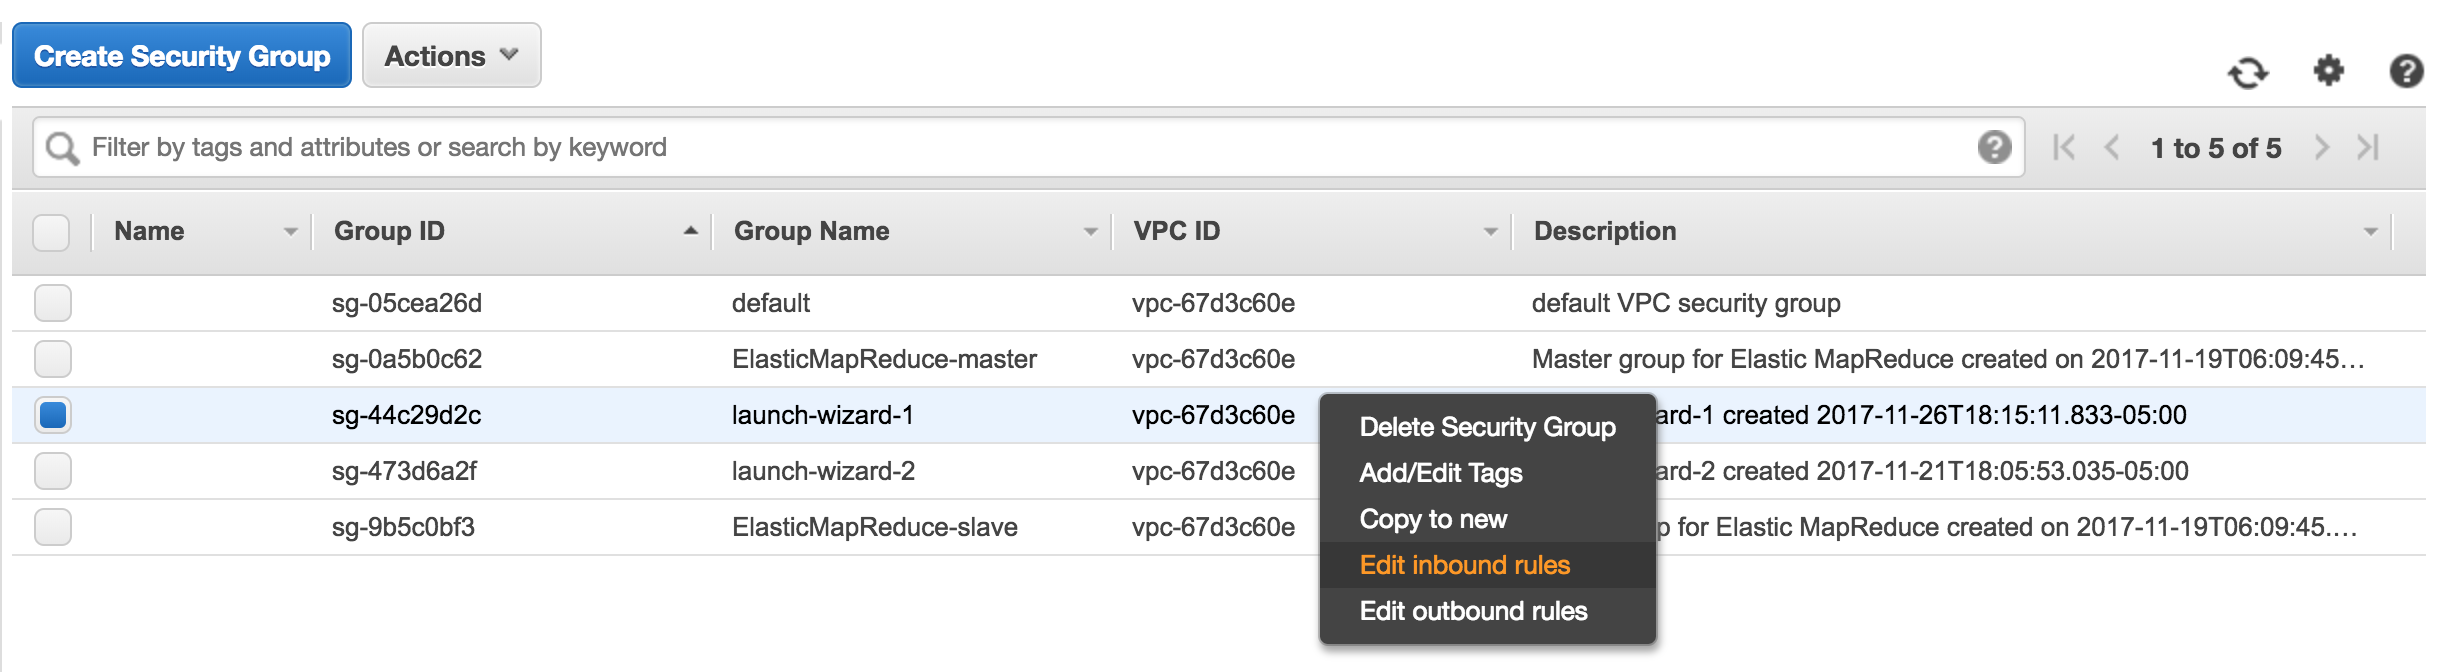
\includegraphics[width=33.86in]{images/ch6_aws_inbound_rules} 

}

\end{figure}

We can now connect to RStudio server:

\url{http://ec2-18-217-97-206.us-east-2.compute.amazonaws.com:8787/}

\begin{figure}

{\centering 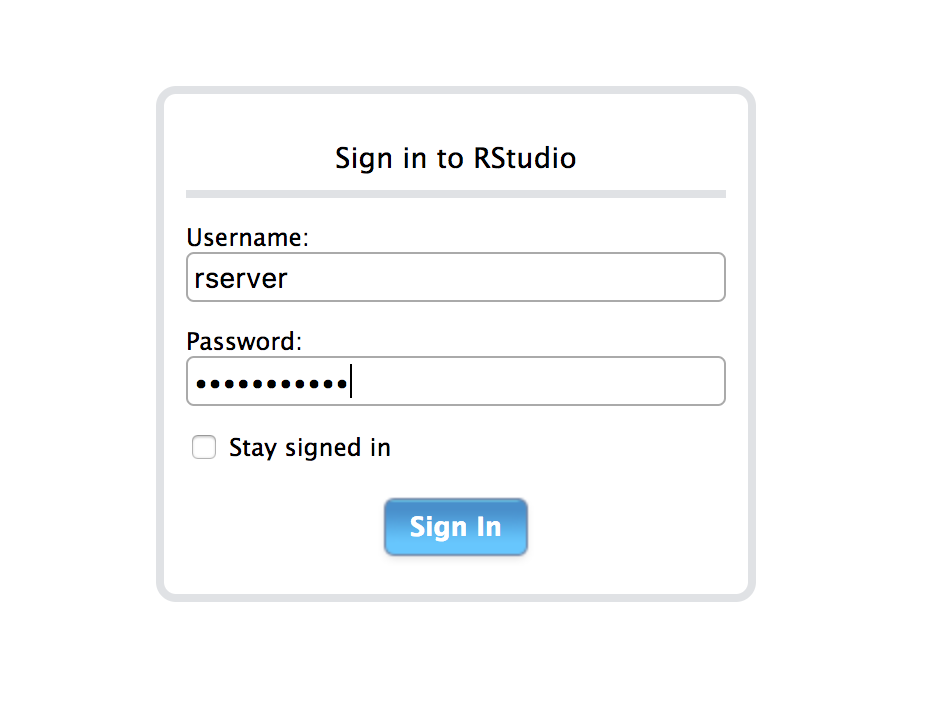
\includegraphics[width=12.94in]{images/ch6_aws_rstudio_signin} 

}

\end{figure}

\section{Spark on AWS: Amazon Elastic MapReduce
(EMR)}\label{spark-on-aws-amazon-elastic-mapreduce-emr}

\url{https://aws.amazon.com/emr/}

\url{https://aws.amazon.com/blogs/big-data/running-sparklyr-rstudios-r-interface-to-spark-on-amazon-emr/}

\subsection{Amazon S3}\label{amazon-s3}

GUI or CLI

\subsection{Amazon CLI}\label{amazon-cli}

\url{https://aws.amazon.com/cli/}

\chapter{Visualization}\label{visualization}

\section{Maps and GIS}\label{maps-and-gis}

\subsection{Longitudes, latitudes and
CRS}\label{longitudes-latitudes-and-crs}

\subsection{Shapefiles}\label{shapefiles}

\subsection{Backends}\label{backends}

\subsubsection{\texorpdfstring{\texttt{gdal}}{gdal}}\label{gdal}

\subsubsection{\texorpdfstring{\texttt{geos}}{geos}}\label{geos}

\subsection{R packages}\label{r-packages}

\subsubsection{\texorpdfstring{\texttt{sp}}{sp}}\label{sp}

\subsubsection{\texorpdfstring{\texttt{sf}}{sf}}\label{sf}

\subsubsection{\texorpdfstring{\texttt{ggmap}}{ggmap}}\label{ggmap}

\subsubsection{\texorpdfstring{\texttt{leaflet}}{leaflet}}\label{leaflet}

\subsubsection{\texorpdfstring{\texttt{Shiny}}{Shiny}}\label{shiny}

\section{Principles of visualization}\label{principles-of-visualization}

Guest lecture (James Honaker)

\bibliography{book.bib,packages.bib}


\end{document}
